% Options for packages loaded elsewhere
\PassOptionsToPackage{unicode}{hyperref}
\PassOptionsToPackage{hyphens}{url}
%
\documentclass[
  12pt,
]{article}
\usepackage{amsmath,amssymb}
\usepackage{lmodern}
\usepackage{iftex}
\ifPDFTeX
  \usepackage[T1]{fontenc}
  \usepackage[utf8]{inputenc}
  \usepackage{textcomp} % provide euro and other symbols
\else % if luatex or xetex
  \usepackage{unicode-math}
  \defaultfontfeatures{Scale=MatchLowercase}
  \defaultfontfeatures[\rmfamily]{Ligatures=TeX,Scale=1}
\fi
% Use upquote if available, for straight quotes in verbatim environments
\IfFileExists{upquote.sty}{\usepackage{upquote}}{}
\IfFileExists{microtype.sty}{% use microtype if available
  \usepackage[]{microtype}
  \UseMicrotypeSet[protrusion]{basicmath} % disable protrusion for tt fonts
}{}
\makeatletter
\@ifundefined{KOMAClassName}{% if non-KOMA class
  \IfFileExists{parskip.sty}{%
    \usepackage{parskip}
  }{% else
    \setlength{\parindent}{0pt}
    \setlength{\parskip}{6pt plus 2pt minus 1pt}}
}{% if KOMA class
  \KOMAoptions{parskip=half}}
\makeatother
\usepackage{xcolor}
\IfFileExists{xurl.sty}{\usepackage{xurl}}{} % add URL line breaks if available
\IfFileExists{bookmark.sty}{\usepackage{bookmark}}{\usepackage{hyperref}}
\hypersetup{
  pdftitle={Factors affecting reliablity of state-space age-structured assessment models},
  pdfauthor={Timothy J. Miller1,2; Greg Britten3; Elizabeth N. Brooks2; Gavin Fay4; Alex Hansell2; Christopher M. Legault2; Brandon Muffley5; Brian C. Stock6; John Wiedenmann7},
  hidelinks,
  pdfcreator={LaTeX via pandoc}}
\urlstyle{same} % disable monospaced font for URLs
\usepackage[margin=1in]{geometry}
\usepackage{graphicx}
\makeatletter
\def\maxwidth{\ifdim\Gin@nat@width>\linewidth\linewidth\else\Gin@nat@width\fi}
\def\maxheight{\ifdim\Gin@nat@height>\textheight\textheight\else\Gin@nat@height\fi}
\makeatother
% Scale images if necessary, so that they will not overflow the page
% margins by default, and it is still possible to overwrite the defaults
% using explicit options in \includegraphics[width, height, ...]{}
\setkeys{Gin}{width=\maxwidth,height=\maxheight,keepaspectratio}
% Set default figure placement to htbp
\makeatletter
\def\fps@figure{htbp}
\makeatother
\setlength{\emergencystretch}{3em} % prevent overfull lines
\providecommand{\tightlist}{%
  \setlength{\itemsep}{0pt}\setlength{\parskip}{0pt}}
\setcounter{secnumdepth}{5}
\newlength{\cslhangindent}
\setlength{\cslhangindent}{1.5em}
\newlength{\csllabelwidth}
\setlength{\csllabelwidth}{3em}
\newlength{\cslentryspacingunit} % times entry-spacing
\setlength{\cslentryspacingunit}{\parskip}
\newenvironment{CSLReferences}[2] % #1 hanging-ident, #2 entry spacing
 {% don't indent paragraphs
  \setlength{\parindent}{0pt}
  % turn on hanging indent if param 1 is 1
  \ifodd #1
  \let\oldpar\par
  \def\par{\hangindent=\cslhangindent\oldpar}
  \fi
  % set entry spacing
  \setlength{\parskip}{#2\cslentryspacingunit}
 }%
 {}
\usepackage{calc}
\newcommand{\CSLBlock}[1]{#1\hfill\break}
\newcommand{\CSLLeftMargin}[1]{\parbox[t]{\csllabelwidth}{#1}}
\newcommand{\CSLRightInline}[1]{\parbox[t]{\linewidth - \csllabelwidth}{#1}\break}
\newcommand{\CSLIndent}[1]{\hspace{\cslhangindent}#1}
\usepackage{url}
\usepackage{setspace}
%\singlespacing
%\onehalfspacing
\doublespacing
\usepackage{lineno}
\linenumbers
\usepackage[belowskip=0pt,aboveskip=0pt]{caption}
\usepackage{relsize}
\usepackage{float}
\usepackage{lscape}
\usepackage{longtable}
\usepackage{amsmath,rotating}
\usepackage[scanall]{psfrag}
\usepackage{bm}
\usepackage{caption,graphics}
\usepackage{graphicx}
\usepackage{sectsty}
\usepackage{color}
\usepackage{fancyhdr}
\usepackage{xspace}
\usepackage{textcomp}
\usepackage{upgreek}
\renewcommand\figurename{Fig.}
\captionsetup{labelsep=period, singlelinecheck=false}
\newcommand{\changesize}[1]{\fontsize{#1pt}{#1pt}\selectfont}
\renewcommand{\arraystretch}{1.5}
%\renewcommand\theadfont{}

\newcommand{\Fmsy}{\ensuremath{F_{\text{MSY}}}\xspace}
\newcommand{\Fspr}[1]{\ensuremath{F_{\text{{#1}\%}}}\xspace}
\newcommand{\afrb}{Alaska Fishery Research Bulletin\xspace}
\newcommand{\ajms}{African Journal of Marine Science\xspace}
\newcommand{\amb}{Advances in Marine Biology\xspace}
\newcommand{\bms}{Bulletin of Marine Science\xspace}
\newcommand{\bjssf}{Bulletin of the Japanese Society of Scientific Fisheries\xspace}
\newcommand{\cb}{Conservation Biology\xspace}
\newcommand{\cjfas}{Canadian Journal of Fisheries and Aquatic Sciences\xspace}
\newcommand{\ea}{Ecological Applications\xspace}
\newcommand{\eer}{Evolutionary Ecology Research\xspace}
\newcommand{\elet}{Ecology Letters\xspace}
\newcommand{\emod}{Ecological Modelling\xspace}
\newcommand{\ebf}{Environmental Biology of Fishes\xspace}
\newcommand{\ff}{Fish and Fisheries\xspace}
\newcommand{\fo}{Fisheries Oceanography\xspace}
\newcommand{\fr}{Fisheries Research\xspace}
\newcommand{\fb}{Fishery Bulletin\xspace}
\newcommand{\ijms}{ICES Journal of Marine Science\xspace}
\newcommand{\iccat}{Collective Volume of Scientific Papers ICCAT\xspace}
\newcommand{\jae}{Journal of Animal Ecology\xspace}
\newcommand{\jai}{Journal of Applied Ichthyology\xspace}
\newcommand{\jdc}{Journal Du Conseil International Pour L'exploration De La Mer\xspace}
\newcommand{\jdcp}{Journal Du Conseil Permanent International Pour L'exploration De La Mer\xspace}
\newcommand{\jembe}{Journal of Experimental Marine Biology and Ecology\xspace}
\newcommand{\jfb}{Journal of Fish Biology\xspace}
\newcommand{\jsr}{Journal of Sea Research\xspace}
\newcommand{\jtb}{Journal of Theoretical Biology\xspace}
\newcommand{\jfrbc}{Journal of the Fisheries Research Board of Canada\xspace}
\newcommand{\jnwafs}{Journal of Northwest Atlantic Fisheries Science\xspace}
\newcommand{\mcf}{Marine and Coastal Fisheries: Dynamics, Management, and Ecosystem Science\xspace}
\newcommand{\mb}{Marine Biology\xspace}
\newcommand{\meps}{Marine Ecology Progress Series\xspace}
\newcommand{\mfr}{Marine Fisheries Review\xspace}
\newcommand{\mpb}{Marine Pollution Bulletin\xspace}
\newcommand{\najfm}{North American Journal of Fisheries Management\xspace}
\newcommand{\nzjmfr}{New Zealand Journal of Marine and Freshwater Research\xspace}
\newcommand{\pnas}{Proceedings of the National Academy of Sciences USA\xspace}
\newcommand{\rpvrciemm}{Rapports et Proc\`es-Verbaux des R\'eunions. Conseil Internationale pour l'Exploration de la Mer\xspace}
\newcommand{\rpvrcpiemm}{Rapports et Proc\`es-Verbaux des R\'eunions. Conseil Permanent Internationale pour l'Exploration de la Mer\xspace}
\newcommand{\rfbf}{Reviews in Fish Biology and Fisheries\xspace}
\newcommand{\sajms}{South African Journal of Marine Science\xspace}
\newcommand{\tafs}{Transactions of the American Fisheries Society\xspace}

\newcommand{\anzjs}{Australian \& New Zealand Journal of Statistics\xspace}
\newcommand{\as}{Applied Statistics\xspace}
\newcommand{\csda}{Computational Statistics \& Data Analysis\xspace}
\newcommand{\ees}{Environmental and Ecological Statistics\xspace}
\newcommand{\jas}{Journal of Applied Statistics\xspace}
\newcommand{\jabes}{Journal of Agricultural, Biological, and Environmental Statistics\xspace}
\newcommand{\jasa}{Journal of the American Statistical Association\xspace}
\newcommand{\jrssb}{Journal of the Royal Statistical Society. Series B\xspace}
\newcommand{\sm}{Statistics in Medicine}

\usepackage{booktabs}
\usepackage{longtable}
\usepackage{array}
\usepackage{multirow}
\usepackage{wrapfig}
\usepackage{float}
\usepackage{colortbl}
\usepackage{pdflscape}
\usepackage{tabu}
\usepackage{threeparttable}
\usepackage{threeparttablex}
\usepackage[normalem]{ulem}
\usepackage{makecell}
\usepackage{xcolor}
\ifLuaTeX
  \usepackage{selnolig}  % disable illegal ligatures
\fi

\title{Factors affecting reliablity of state-space age-structured
assessment models}
\author{Timothy J. Miller\textsuperscript{1,2} \and Greg
Britten\textsuperscript{3} \and Elizabeth N.
Brooks\textsuperscript{2} \and Gavin Fay\textsuperscript{4} \and Alex
Hansell\textsuperscript{2} \and Christopher M.
Legault\textsuperscript{2} \and Brandon
Muffley\textsuperscript{5} \and Brian C.
Stock\textsuperscript{6} \and John Wiedenmann\textsuperscript{7}}
\date{15 January, 2025}

\begin{document}
\maketitle

\(^1\)corresponding author:
\href{mailto:timothy.j.miller@noaa.gov}{\nolinkurl{timothy.j.miller@noaa.gov}}\\
\(^2\)Northeast Fisheries Science Center, Woods Hole Laboratory, 166
Water Street, Woods Hole, MA 02543 USA\\
\(^3\)Woods Hole Oceanographic Institution\\
\(^4\)SMAST\\
\(^5\)Institute of Marine Research\\
\(^6\)Mid-Atlantic Fisheries Management Council\\
\(^7\)Rutgers University\\

\pagebreak

\hypertarget{abstract}{%
\subsection*{Abstract}\label{abstract}}
\addcontentsline{toc}{subsection}{Abstract}

Random effects can be included in state-space assessment models on many
processes and in many ways, and guidance is needed on statistical
reliability and model selection criteria. We simulated 72 operating
models with varying fishing history, observation error uncertainty, and
process error magnitude, correlation, and source (recruitment, survival,
fishery selectivity, catchability, and natural mortality). We fit
estimating models with different assumptions on the process error
source, whether (mean) natural mortality was estimated, and whether a
stock-recruit relationship was estimated.

Models that assumed the correct process error source had high
convergence and low bias. Bias was also low under most process error
assumptions when there was contrast in fishing pressure.
Stock-recruitment parameters were only reliably estimated in ideal
situations. Marginal AIC most accurately distinguished process errors on
recruitment, survival, and selectivity, as well as larger magnitude
process errors of other types. Retrospective patterns were generally
weak except for recruitment when observation error was high, even with
the correct process error assumptions. When models did exhibit some
retrospective pattern, estimating natural mortality often removed it.

\pagebreak

\pagebreak

\hypertarget{introduction}{%
\section*{Introduction}\label{introduction}}
\addcontentsline{toc}{section}{Introduction}

Application of state-space models in fisheries stock assessment and
management has expanded dramatically within ICES, Canada, and the
Northeast US (Nielsen and Berg 2014; Cadigan 2016; Pedersen and Berg
2017; Stock and Miller 2021). State-space approaches that use random
effects to parameterize process errors is considered best practice and a
requirement for the next generation of stock assessment models (Hoyle et
al. 2022; Punt 2023).

Much is known about the reliability of state-space models that are
linear or Gaussian (Aeberhard et al. 2018), but applications in
fisheries management are nonlinear and typically include multiple types
of observations with varying distributional assumptions. Furthermore,
there is a wide range of potential random effects structures and model
parameters that can be treated as random effects in assessment models.
We know relatively little about the factors affecting statistical
reliability of such models or the ability of information criteria to
distinguish among such alternative structures.

Li et al. (2024) investigated some aspects of inferences for operating
models with multiple sources of process error, but there are differences
for this paper.

Here we conduct a simulation study with operating models (OMs) varying
by degree of observation error uncertainty, source and variability of
process error, and fishing history. The simulations from these OMs are
fitted with estimation models (EMs) that make alternative assumptions
for sources of process error, whether a stock-recruit model was
estimated, and whether M is estimated. We evaluate whether AIC can
correctly determine the correct source of process error and stock
effects on recruitment. We also evaluate the degree of bias in the
outputs of the assessment model that are important for management.

\hypertarget{methods}{%
\section*{Methods}\label{methods}}
\addcontentsline{toc}{section}{Methods}

We used the Woods Hole Assessment Model (WHAM) to configure operating
and EMs in our simulation study (Miller and Stock 2020; Stock and Miller
2021). WHAM is an R package freely available as a github repository. For
this study we used
\href{https://github.com/timjmiller/wham/tree/77bbd946e4881216a439933473d1c58b21c270c3}{version
1.0.6.9000, commit 77bbd94}. This package has also been used to
configure operating and EMs for closed loop simulations evaluating
index-based assessment methods (Legault et al. 2023) and is used for
management of haddock, butterfish, American plaice, bluefish, Atlantic
cod, black sea bass, and yellowtail flounder in the Northeast US.

We completed a simulation study with a number of OMs that can be
categorized based on where process error random effects are assumed:
abundance at age (R, R+S), natural mortality (R+M), fleet selectivity
(R+Sel), or index catchability (R+q). For each OM assumption about
variance of process errors and observations are required and the values
we used were based on a review of the range of estimates from
applications of WHAM in management of stocks of haddock, butterfish, and
American plaice in the NE US.

In total, we configured 72 OMs with alternative assumptions about the
source and variability of process errors, level of observation error in
indices and age composition data, and contrast in fishing pressure over
time. We fitted 20 EMs to observations from each of 100 simulations
where process errors were also simulated. EMs made alternative
assumptions about the source of process errors and whether natural
mortality (or the mean for models with process error in natural
mortality) was estimated and whether a Beverton-Holt stock recruit
relationship was estimated within the EM. Details of each of the
operating and EMs are described below.

We did not use the log-normal bias-correction feature for process errors
or observations described by (Stock and Miller 2021) for operating and
EMs (Li et al. In review). Simulations and model fitting were all
carried out on the University of Massachusetts Green High-Performance
Computing Cluster. All code we used to perform the simulation study and
summarize results can be found at
\url{https://github.com/timjmiller/SSRTWG/tree/main/Project_0/code}.

\hypertarget{operating-models}{%
\subsection*{Operating models}\label{operating-models}}
\addcontentsline{toc}{subsection}{Operating models}

\hypertarget{population}{%
\subsubsection*{Population}\label{population}}
\addcontentsline{toc}{subsubsection}{Population}

The population consists of 10 age classes: ages 1 to 10+ and we assume
spawning occurs each year 1/4 of the way through the year. The maturity
at age was a logistic curve with \(a_{50}\) = 2.89 and slope = 0.88
(Figure \ref{om_maturity}).

Weight at age was generated with a von Bertalanffy growth function \[
L_a = L_{\infty}\left(1 - e^{-k(a - t_0)}\right)
\] where \(t_0 = 0\), \(L_\infty = 85\), and \(k = 0.3\), and a L-W
relationship such that \[
W_a = \theta_1 L_a^{\theta_2}
\] where \(\theta_1 = e^{-12.1}\) and \(\theta_2 = 3.2\) (Figure
\ref{om_waa}).

We assumed a Beverton-Holt stock recruit function with constant
pre-recruit mortality parameters for all OMs. All post-recruit
productivity components are constant in the NAA and survey catchability
process error OMs. Therefore steepness and unfished recruitment are also
constant over the time period for those OMs (Miller and Brooks 2021). We
specified unfished recruitment = \(R_0 = e^{10}\) and
\(\Fmsy = F_{40\%} = 0.348\) equated to a steepness of 0.69 and
\(\alpha=0.60\) and \(\beta = 2.4 \times 10^{-5}\) for the \[
N_{1,y} = \frac{\alpha \text{SSB}_{y-1}}{1 + \beta \text{SSB}_{y-1}} 
\] Beverton-Holt parameterization (Figure \ref{om_sr}). For OMs without
process errors on natural mortality we assumed the rate was assumed 0.2.
For OMs with process errors on natural mortality the mean log natural
mortality rate was \(\log(0.2)\).

We used two fishing scenarios for OMs. In the first scenario, the stock
experiences overfishing at 2.5\Fmsy for the first 20 years and fishing
at \Fmsy for the last 20 years (denoted \(2.5\Fmsy \rightarrow \Fmsy\)).
In the second scenario, the stock is fished at \Fmsy for the entire time
period. The magnitude of the overfishing assumptions is based on average
estimates of overfishing for NE groundfish stocks from (Wiedenmann et
al. 2019). Legault et al. (2023) also used similar approaches to
defining fishing mortality histories for OMs.

We specified initial population abundance at age at the equilibrium
distribution fishing at either \(F = 2.5\times \Fmsy\) or \(F = \Fmsy\)
for the two alternative fishing histories. This implies that, for a
deterministic model, the abundance at age would not change from the
first year to the next.

For OMs with time-varying random effects for M, steepness is not
constant, but we used the same alpha and beta parameters as other OMs
this equates to a steepness and R0 at the median of the time series
process for M. For OMs with time-varying random effects for fishery
selectivity, \Fmsy is also not constant however we use the same F
history as other OMs which corresponds to Fmsy at the mean selectivity
parameters.

\hypertarget{fleets}{%
\subsubsection*{Fleets}\label{fleets}}
\addcontentsline{toc}{subsubsection}{Fleets}

We assumed a single fleet operating year round for catch observations
with logistic selectivity for the fleet with \(a_{50} = 5\) and slope =
1 (Figure \ref{om_mean_selectivity}). This selectivity is was used to
define \Fmsy for the Beverton-Holt stock recruitment parameters above.
We assumed a logistic-normal distribution for the age-composition
observations for the fleet.

\hypertarget{indices}{%
\subsubsection*{Indices}\label{indices}}
\addcontentsline{toc}{subsubsection}{Indices}

Two time series of surveys are assumed and observed in numbers rather
than biomass for the entire 40 year period with one occurring in the
spring (0.25 of each year) and one in the fall (0.75 of each year).
Catchability of both surveys are assumed to be 0.1. Like the fishing
fleet, we assumed logistic selectivity for both indices with
\(a_{50} = 5\) and slope = 1 and a logistic-normal distribution for the
age-composition observations.

\hypertarget{observation-uncertainty}{%
\subsubsection*{Observation Uncertainty}\label{observation-uncertainty}}
\addcontentsline{toc}{subsubsection}{Observation Uncertainty}

Standard deviation for log-aggregate catch was 0.1. There were two
levels of observation error variance for indices and age composition for
both indices and fleet catch. A low uncertainty specification assumed
standard deviation of both series of log-aggregate index observations
was 0.1 and the standard deviation of the logistic-normal for age
composition observations was 0.3 In the high uncertainty specification
the standard deviation for log-aggregate indices was 0.4 and that for
the age composition observations was 1.5. For all EMs, standard
deviation for log-aggregate observations was assumed known whereas that
for the logistic-normal age composition observations was estimated.

\hypertarget{operating-models-with-random-effects-on-numbers-at-age}{%
\subsubsection*{Operating models with random effects on numbers at
age}\label{operating-models-with-random-effects-on-numbers-at-age}}
\addcontentsline{toc}{subsubsection}{Operating models with random
effects on numbers at age}

For operating models with random effects on recruitment and(or) survival
(R, R+S) we assumed marginal standard deviations for recruitment of
\(\sigma_R \in \{0.5,1.5\}\) and marginal standard deviations for older
age classes of \(\sigma_{2+} \in \{0,0.25, 0.5\}\). The full factorial
combination of these process error assumptions and fishing history (2
levels) and observation error (2 levels) scenarios described above
results in 24 different R (\(\sigma_{2+} = 0\)) and R+S operating models
(Table \ref{naa_om_table}).

\hypertarget{operating-models-with-random-effects-on-natural-mortality}{%
\subsubsection*{Operating models with random effects on natural
mortality}\label{operating-models-with-random-effects-on-natural-mortality}}
\addcontentsline{toc}{subsubsection}{Operating models with random
effects on natural mortality}

All R+M OMs treat natural mortality constant across age, but with
annually varying random effects. WHAM treats natural mortality as a
log-transformed parameter \[
\log M_{y,a} = \mu_{M} + \epsilon_{M,y}
\] that is a linear combination of a mean that is constant across ages
\(\mu_{M} = \log(0.2)\) and any annual random effects marginally
distributed as
\(\epsilon_{M,y} \sim \text{N}\left(0,\sigma_M^2\right)\). Uncorrelated
random effects were also included on recruitment with \(\sigma_R = 0.5\)
(hence, R+M). The marginal standard deviations we assumed for log
natural mortality random effects were \(\sigma_M \in \{0.1, 0.5\}\) and
AR1 autocorrelation parameters of \(\rho_M \in \{0,0.9\}\). The full
factorial combination of these process error assumptions and fishing
history (2 levels) and observation error (2 levels) scenarios described
above results in 16 different R+M OMs (Table \ref{M_om_table}).

\hypertarget{operating-models-with-random-effects-on-fleet-selectivity}{%
\subsubsection*{Operating models with random effects on fleet
selectivity}\label{operating-models-with-random-effects-on-fleet-selectivity}}
\addcontentsline{toc}{subsubsection}{Operating models with random
effects on fleet selectivity}

MORE SPECIFICS about correlation of random effects? Both selectivity
pars? just correlated by year? WHAM treats selectivity parameter \(s\)
as a logit-transformed parameter \[
\log\left(\frac{p_{s,y}-l_{s}}{u_{s}-p_{s,y}}\right) = \mu_s + \epsilon_{s,y}
\] that is a linear combination of a mean \(\mu_s\) and any annual
random effects marginally distributed as
\(\epsilon_{s,y} \sim \text{N}\left(0,\sigma_s^2\right)\) where the
lower and upper bounds of the parameter (\(l_s\) and \(u_s\)) can be
specified by the user. All selectivity parameters are either \(a_50\) or
slope parameters and we assume bounds of 0 and 10 for all selectivity
parameters for all operating and EMs. The marginal standard deviations
we assumed for logit scale random effects were
\(\sigma_s \in \{0.1, 0.5\}\) and AR1 autocorrelation parameters of
\(\rho_s \in \{0,0.9\}\). Like R+M OMs, the full factorial combination
of these process error assumptions and fishing history (2 levels) and
observation error (2 levels) scenarios described above results in 16
different R+Sel OMs (Table \ref{sel_om_table}).

\hypertarget{operating-models-with-random-effects-on-index-catchability}{%
\subsubsection*{Operating models with random effects on index
catchability}\label{operating-models-with-random-effects-on-index-catchability}}
\addcontentsline{toc}{subsubsection}{Operating models with random
effects on index catchability}

Like selectivity parameters, WHAM treats catchability for an index \(i\)
as a logit-transformed parameter \[
\log\left(\frac{q_{i,y}-l_{i}}{u_{i}-q_{i,y}}\right) = \mu_i + \epsilon_{i,y}
\] that is a linear combination of a mean \(\mu_i\) and any annual
random effects marginally distributed as
\(\epsilon_{i,y} \sim \text{N}\left(0,\sigma_i^2\right)\) where the
lower and upper bounds of the catchability (\(l_i\) and \(u_i\)) can be
specified by the user. Here we assume bounds of 0 and 1000 for all
operating and EMs. For operating and EMs with process errors on
catchability, the temporal variation is only assumed for the first
index. The marginal standard deviations we assumed for logit scale
random effects were \(\sigma_i \in \{0.1, 0.5\}\) and AR1
autocorrelation parameters of \(\rho_i \in \{0,0.9\}\). Like R+M and
R+Sel OMs, the full factorial combination of these process error
assumptions and fishing history (2 levels) and observation error (2
levels) scenarios described above results in 16 different R+q OMs (Table
\ref{q_om_table}).

\hypertarget{estimation-models}{%
\subsection*{Estimation models}\label{estimation-models}}
\addcontentsline{toc}{subsection}{Estimation models}

For each data set simulated from an OM 20 EMs were fit. A total of 32
different EMs were fit across all OMs where the subset of 20 depended on
the source of process error (Table \ref{em_table}). The first 20 EMs in
Table \ref{em_table} were fit to simulate data sets from R and R+S OMs.
EMs 5 to 24 in Table \ref{em_table} were fit to simulate data sets from
R+M OMs. EMs 5 to 20 and 25-28 in Table \ref{em_table} were fit to
simulate data sets from R+Sel OMs. Finally, EMs 5 to 20 and 29-32 in
Table \ref{em_table} were fit to simulate data sets from R+q OMs. The
observation error variance of aggregate catch and indices were all
assumed known at the true values.

maturity, weight at age, index and catch CVs, assumed known in all EMs

\hypertarget{measures-of-reliability}{%
\subsection*{Measures of reliability}\label{measures-of-reliability}}
\addcontentsline{toc}{subsection}{Measures of reliability}

The first measure of reliability we investigated was frequency of
convergence when fitting each EM to the simulated data sets. There are
various ways to assess convergence of the fit. We summarized 5
alternative categories of convergence.

\begin{enumerate}
\def\labelenumi{\arabic{enumi}.}
\tightlist
\item
  Fit complete: Did the optimization routine (stats::nlminb) complete
  without error?
\item
  No flag: Did the stats::nlminb convergence flag = 0 indicate
  successful convergence?
\item
  Good gradient: Was the maximum absolute value of the gradient of the
  log-likelihood \textless{} \(1\times10^{-6}\)?
\item
  No SE NAs: Did TMB::sdreport provide non-NA values for all fixed
  effects standard errors?
\item
  No big SEs: Did TMB::sdreport provide all standard errors \textless{}
  100?
\end{enumerate}

The first convergence criterion assesses whether the model crashes. The
third is a measure that assesses how flat the likelihood is at the
optimized point of the likelihood surface. The fourth and fifth criteria
are specific to the hessian-based standard error reporting provided by
TMB. the TMB::sdreport function will sometimes return standard error
estimates even when the calculated hessian is not invertible (fourth
criterion). It will also provide large standard errors for some
parameters that are not estimated well or are near bounds on the
transformed scale that is of primary interest. For example, variance
parameters for random effects can often be estimated near 0 when the fit
suggests no variation in the random effects or, equivalently, that the
model without random effects is better. Note that Types 2 through 5 also
require type 1, and type 5 requires type 4. We used the Clopper-Pearson
exact method for constructing 95\% confidence intervals of the
probabilities of convergence (Clopper and Pearson 1934; Thulin 2014).

\hypertarget{aic-for-model-selection}{%
\subsubsection*{AIC for model selection}\label{aic-for-model-selection}}
\addcontentsline{toc}{subsubsection}{AIC for model selection}

We estimated the probability of selection of each process error model
structure (R, R+S, R+M, R+Sel, R+q) using marginal AIC. For a given
operating model, we compared AIC for EMs that all made the same
assumptions about median/constant natural mortality (known or estimated)
and stock recruitment model (Beverton-Holt or none).

We also estimated the probability of correctly selecting between models
with Beverton-Holt stock recruit function assumed and models without the
stock-recruit function (null model). We made these comparisons between
models that otherwise assume the same process error structure as the
operating model and both of the compared models either estimate
median/constant natural mortality or assume it is known. Our preliminary
inspections of the proportions of simulations where the correct
recruitment model was chosen for a given set of OM factors indicated
generally poor performance of AIC. Furthermore, it has been shown that
estimation of stock-recruit parameters requires a wide range of SSB
(References). Therefore, we fit logistic regression models to the
indicator of Beverton-Holt models having lower AIC as a function of the
log-standard deviation of the true log(SSB) (similar to the log of the
coefficient of variation for SSB) for each simulation.

All results only condition on whether all of the compared estimating
models completed the optimization process without failure. We did not
condition on convergence as defined by a gradient threshold or
invertibity of the hessian because optimization can correctly determine
the the correct likelihood that would indicate poor convergence because
variance parameters may be at the lower bound of zero correctly for
models that assume the incorrect process error structure.

\hypertarget{bias}{%
\subsubsection*{Bias}\label{bias}}
\addcontentsline{toc}{subsubsection}{Bias}

We estimated bias as the median of the relative errors across all
simulations for a given OM and EM combination. \[
\text{RE}\left(\theta_i\right) = \frac{\widehat \theta_i - \theta_i}{\theta_i}
\] of annual SSB and fully-selected fishing mortality for each EM and
constructed 95\% confidence intervals for the median relative bias using
the binomial distribution approach as in Miller and Hyun (2018) and
Stock and Miller (2021). We also estimated bias of stock-recruit
parameters for EMs that assumed the Beverton-Holt stock recruit function
and the mean natural mortality rate parameter when estimated.

Similar to the AIC results, bias results only condition on whether the
estimating model completed the optimization process without failure. We
did not condition on convergence as defined by a gradient threshold or
invertibity of the hessian because the optimized model can provide
reliable estimation of SSB, F, M, and stock recruit parameters whether
or not the model was able to estimate non-zero random effects. In
practice, the model would be reconfigured to remove unnecessary process
errors and produce otherwise equivalent parameter estimates.

\hypertarget{mohns-rho}{%
\subsubsection*{\texorpdfstring{Mohn's
\(\rho\)}{Mohn's \textbackslash rho}}\label{mohns-rho}}
\addcontentsline{toc}{subsubsection}{Mohn's \(\rho\)}

We estimated Mohn's \(\rho\) for SSB, fully-selected fishing mortality,
and recruitment for each EM. We estimated 7 peels for each EM. We
calculated median 95\% confidence intervals for Mohn's \(\rho\) using
the same methods as that for relative bias.

Similar to the other results, retrospective results only condition on
whether all of the peels of a given estimating model completed the
optimization process without failure. We did not condition on
convergence as defined by a gradient threshold or invertibity of the
hessian because the optimized model can provide reliable estimation of
SSB, F, M, and stock recruit parameters whether or not the model was
able to estimate non-zero random effects.

\hypertarget{results}{%
\section*{Results}\label{results}}
\addcontentsline{toc}{section}{Results}

\hypertarget{convergence-performance}{%
\subsection*{Convergence performance}\label{convergence-performance}}
\addcontentsline{toc}{subsection}{Convergence performance}

\hypertarget{r-rs-operating-models}{%
\subsubsection*{R, R+S operating models}\label{r-rs-operating-models}}
\addcontentsline{toc}{subsubsection}{R, R+S operating models}

R+S EMs fit to R OMs exhibited poor convergence for types 3, 4, and 5
regardless of whether M or a stock-recruit relationship was estimated
(Figures \ref{naa_om_em_R_MF_convergence} to
\ref{naa_om_em_BH_ME_convergence}). R EMs exhibited high convergence
rates for all convergence types for both R and R+S OMs. Convergence
rates were high for all convergence types for all EMs in R+S OMs with
lower uncertainty in observations. Convergence for most convergence
types generally declines most EMs when mean-log natural mortality rate
is estimated and/or a Beverton-Holt stock recruit relationship is
estimated even when the process error assumptions of the estimation and
OMs match. There can be relatively high convergence probability of type
4 (an invertible hessian) for EMs that do not have the correct process
error assumed, but type 5 convergence (no very large standard errors
estimated from hessian) for these EMs is typically much lower.

\hypertarget{rm-operating-models}{%
\subsubsection*{R+M operating models}\label{rm-operating-models}}
\addcontentsline{toc}{subsubsection}{R+M operating models}

R+S EMs generally converged less reliably across convergence types than
other EMs when fit to data generated from R+M OMs (Figures
\ref{M_om_em_R_MF_convergence} to \ref{M_om_em_BH_ME_convergence}).
However, using convergence type 5, all EMs converged poorly when OMs had
low variability in natural mortality process errors or higher
observation error uncertainty. Using convergence type 5, R+M EMs
generally converged better than other EMs when observation error
uncertainty was low and natural mortality process errors were more
variable. Like R+S OMs, the probability of convergence generally
declined for all EMs when mean log-natural mortality and/or a
stock-recruit relationship was estimated.

\hypertarget{rsel-operating-models}{%
\subsubsection*{R+Sel operating models}\label{rsel-operating-models}}
\addcontentsline{toc}{subsubsection}{R+Sel operating models}

R+S EMs in particular converged poorly when R+Sel OMs had less
variability in selectivity process errors or higher observation error
uncertainty (Figures \ref{Sel_om_em_R_MF_convergence} to
\ref{Sel_om_em_BH_ME_convergence}). R+Sel EMs generally converged better
than other EMs for OMs with greater variability in process errors, lower
observation error, and contrast in fishing pressure regardless of
whether mean log natural mortality or a stock recruit relationship was
estimated.

\hypertarget{rq-operating-models}{%
\subsubsection*{R+q operating models}\label{rq-operating-models}}
\addcontentsline{toc}{subsubsection}{R+q operating models}

Convergence of R+q EMs is generally better than that of other EMs for
all convergence types when R+q OMs assume contrast in fishing history
overFigures (\ref{q_om_em_R_MF_convergence} to
\ref{q_om_em_BH_ME_convergence}). Convergence of R+S EMs is generally
worse than that of other EMs across all OMs whether or not mean
log-natural mortality or a stock recruit relationship is estimated.
Again, convergence probablity generally declines for all EMs when mean
log-natural mortality or a stock recruit relationship is estimated.

\hypertarget{aic-performance-for-process-error-structure}{%
\subsection*{AIC performance for process error
structure}\label{aic-performance-for-process-error-structure}}
\addcontentsline{toc}{subsection}{AIC performance for process error
structure}

\hypertarget{r-rs-operating-models-1}{%
\subsubsection*{R, R+S operating models}\label{r-rs-operating-models-1}}
\addcontentsline{toc}{subsubsection}{R, R+S operating models}

Marginal AIC accurately determines the correct process error assumptions
in EMs when data are generated from R and R+S OMs, regardless of whether
mean log-natural mortality or a stock recruit relationship is estimated
(Figures \ref{naa_om_proportion_best_aic_R_MF} to
\ref{naa_om_proportion_best_aic_SR_ME}). Adding estimation of mean
log-natural mortality or a stock recruit relationship separately has a
negligible effect on the accuracy of determining the correct process
error assumption. When both are estimated, there is a noticeable
reduction in accuracy when OMs have a constant fishing history,
observation error is low and largest variability in recruitment process
errors.

\hypertarget{rm-operating-models-1}{%
\subsubsection*{R+M operating models}\label{rm-operating-models-1}}
\addcontentsline{toc}{subsubsection}{R+M operating models}

Marginal AIC only accurately determined the correct process error model
and correlation structure when observation error was low and variability
in natural mortality process errors was high (Figures
\ref{M_om_proportion_best_aic_R_MF} to
\ref{M_om_proportion_best_aic_SR_ME}). Estimating the mean natural
mortality rate reduced the accuracy of AIC for OMs that assumed natural
mortality process errors were independent. For OMs with poor accuracy,
AIC most frequently selected EMs with process errors in catchability or
selectivity. Selection of R+S EMs was typically unlikely.

\hypertarget{rsel-operating-models-1}{%
\subsubsection*{R+Sel operating models}\label{rsel-operating-models-1}}
\addcontentsline{toc}{subsubsection}{R+Sel operating models}

Marginal AIC most accurately determined the correct source of process
error and correlation structure for R+Sel OMs with low observation error
(Figures \ref{Sel_om_proportion_best_aic_R_MF} to
\ref{Sel_om_proportion_best_aic_SR_ME}). When there was low variability
in selectivity process errors and high observation error, R+q or R+S EMs
were more likely to have the best AIC. Whether mean log-natural morality
or stock recruit relationships were estimated appeared to have little
effect on the performance of marginal AIC.

\hypertarget{rq-operating-models-1}{%
\subsubsection*{R+q operating models}\label{rq-operating-models-1}}
\addcontentsline{toc}{subsubsection}{R+q operating models}

Marginal AIC most accurately determined the correct source of process
error and correlation structure for R+q OMs with high variability in
catchability process errors (Figures \ref{q_om_proportion_best_aic_R_MF}
to \ref{q_om_proportion_best_aic_SR_ME}). The worst accuracy occurred
for OMs with low variability in catchability process errors and high
observation error. However, in these OMs, the marginal AIC accurately
determined the correct source of process error (but not correlation
structure) except when EMs estimated both mean log-natural morality and
the stock recruit relationships and OMs assumed a constant fishing
pressure.

\hypertarget{aic-performance-for-the-stock-recruit-relationship}{%
\subsection*{AIC performance for the stock-recruit
relationship}\label{aic-performance-for-the-stock-recruit-relationship}}
\addcontentsline{toc}{subsection}{AIC performance for the stock-recruit
relationship}

Our comparisons of model performance condition on assuming the true
process error configuration is known (EM and OM process error
assumptions match). Broadly, we found generally poor accuracy of AIC in
selecting models assuming a Beverton-Holt stock recruit function over
the null model without an assumed stock-recruit relationship for all OMs
(Tables \ref{naa_om_em_R_BH_aic_table} to \ref{q_om_em_R_BH_aic_table}.
However, we also found AIC to more accurately determine a stock-recruit
relationship when there was greater variation in spawning biomass
generated in the simulated populations.

\hypertarget{r-rs-operating-models-2}{%
\subsubsection*{R, R+S operating models}\label{r-rs-operating-models-2}}
\addcontentsline{toc}{subsubsection}{R, R+S operating models}

Among R and R+S OMs, AIC accuracy for including the B-H stock-recruit
relationship was estimated to be highest for R OMs and EMs and lowest
variance of recruitment process errors (Figures
\ref{naa_om_MF_BH_glm_AIC_plots} and \ref{naa_om_ME_BH_glm_AIC_plots}).
FOr R+S OMs and holding variability in SSB constant, accuracy of
stock-recruit model selection declined with greater variance of
recruitment and survival process errors. Simultaneously estimating mean
log-natural mortality has a small negative effect on AIC accuracy, but
there is an improvement in AIC accuracy with lower observation error in
indices and age composition and lower variation of survival process
errors.

\hypertarget{rm-operating-models-2}{%
\subsubsection*{R+M operating models}\label{rm-operating-models-2}}
\addcontentsline{toc}{subsubsection}{R+M operating models}

For R+M OMs and EMs there appeared to be little effect of correlation in
the natural mortality process errors or estimating the mean log-natural
mortality on accuracy of AIC in determining a stock-recruit function,
holding variability in SSB constant (Figures
\ref{M_om_MF_BH_glm_AIC_plots} and \ref{M_om_ME_BH_glm_AIC_plots}).
However, there was an increase in accuracy with lower observation error
for OMs with higher variability in natural mortality process errors
whether the mean natural mortality rate parameter was estimated or not.

\hypertarget{rsel-operating-models-2}{%
\subsubsection*{R+Sel operating models}\label{rsel-operating-models-2}}
\addcontentsline{toc}{subsubsection}{R+Sel operating models}

The range of variation in SSB across simulated populations was lower for
R+Sel OMs than R+S or R+M OMs. OMs with contrast in fishing pressure
over time is the primary mechanism creating variation in SSB. However,
there appears to be little effect of variability or correlation of
selectivity process errors or whether mean log-natural mortality was
estimated on the accuracy of AIC in selecting the stock recruit
relationship (Figures \ref{Sel_om_MF_BH_glm_AIC_plots} and
\ref{Sel_om_ME_BH_glm_AIC_plots}). However, there was an increase in AIC
accuracy with lower observation error for OMs with independent process
errors whether the mean natural mortality rate parameter was estimated
or not.

\hypertarget{rq-operating-models-2}{%
\subsubsection*{R+q operating models}\label{rq-operating-models-2}}
\addcontentsline{toc}{subsubsection}{R+q operating models}

Like the R+Sel OMs, the range of variation in SSB across simulated
populations for R+q OMs is only increased by allowing contrast in
fishing pressure over time. There appears to be a slight decrease in
accuracy in AIC when mean log-natural mortality is estimated and there
is a more noticeable increase in accuracy for OMs with lower observation
error in those cases. (Figures \ref{q_om_MF_BH_glm_AIC_plots} and
\ref{q_om_ME_BH_glm_AIC_plots}). There was also an increase in AIC
accuracy with lower observation error for when the mean natural
mortality rate parameter was estimated.

\hypertarget{bias-1}{%
\subsection*{Bias}\label{bias-1}}
\addcontentsline{toc}{subsection}{Bias}

\hypertarget{r-rs-operating-models-3}{%
\subsubsection*{R, R+S operating models}\label{r-rs-operating-models-3}}
\addcontentsline{toc}{subsubsection}{R, R+S operating models}

When mean log-natural mortality is known, all estimating models
regardless of process error assumptions produce unbiased estimates of
SSB over the entire time period for R OMs (Figure
\ref{naa_om_em_R_MF_relbias_ssb}). For R+S OMs, only R+S EMs produce
unbiased estimation of SSB and bias resulting from other EMs increased
with larger variability in survival random effects. Estimating mean
log-natural mortality generally produced greater variability in relative
errors of SSB estimates and a change in sign of bias for EMs assuming
process errors other than R and R+S (Figure
\ref{naa_om_em_R_ME_relbias_ssb}). Estimating a stock-recruit
relationship had little discernable effect on bias of SSB estimation
(Figures \ref{naa_om_em_BH_MF_relbias_ssb}), but in combination with
estimating mean log-natural mortality resulted in large bias of R+S EMs
for R OMs with high observation error, constant fishing pressure and
large variability in recruitment process errors (Figure
\ref{naa_om_em_BH_ME_relbias_ssb}).

\hypertarget{rm-operating-models-3}{%
\subsubsection*{R+M operating models}\label{rm-operating-models-3}}
\addcontentsline{toc}{subsubsection}{R+M operating models}

When mean log-natural mortality is known, SSB estimation bias was small
or non-existent for all EM process error assumptions when the OMs had
low variability of the natural mortality process errors except a
tendency toward negative bias in the terminal years for OMs with high
observation error and a change in fishing pressure over time (Figure
\ref{M_om_em_R_MF_relbias_ssb}). Errors in SSB estimation were most
variable with high variability and autocorrelation of natural mortality
process errors, but confidence intervals generally covered 0 indicating
no evidence of bias. Estimating mean log-natural mortality results in
large variability in SSB relative errors, particularly for OMs with high
observation error and constant fishing pressure and all EMs produced
biased estimation of SSB over all years when OMs had high observation
error, a change in fishing pressure and low variability of natural
mortality process errors (Figure \ref{M_om_em_R_ME_relbias_ssb}). Like R
and R+S OMs, estimating a stock-recruit relationship had little
discernible effect on SSB bias (Figures \ref{M_om_em_BH_MF_relbias_ssb}
and \ref{M_om_em_BH_ME_relbias_ssb}).

\hypertarget{rsel-operating-models-3}{%
\subsubsection*{R+Sel operating models}\label{rsel-operating-models-3}}
\addcontentsline{toc}{subsubsection}{R+Sel operating models}

When mean log-natural mortality is known and no stock-recruit
relationship was estimated, SSB estimation bias was low for all EM
process error assumptions (Figure \ref{Sel_om_em_R_MF_relbias_ssb}). The
worst bias occurred for OMs with uncorrelated by more variable
selectivity process errors and high observations error. As for other
OMs, estimating mean log-natural mortality resulted in greater
variability of the relative errors in SSB, but also more evidence of
bias for EMS without the correct process error assumption (Figure
\ref{Sel_om_em_R_ME_relbias_ssb}). Estimating a stock recruit
relationship resulted in greater estimation of SSB in the terminal years
and sometimes less bias when OMs had high observation error and a change
in fishing pressure over time and the effect was more pronounced when
mean log-natural mortality was estimated (Figures
\ref{Sel_om_em_BH_MF_relbias_ssb} and
\ref{Sel_om_em_BH_ME_relbias_ssb}).

\hypertarget{rq-operating-models-3}{%
\subsubsection*{R+q operating models}\label{rq-operating-models-3}}
\addcontentsline{toc}{subsubsection}{R+q operating models}

When mean log-natural mortality is known and no S-R relationship was
estimated, SSB estimation bias was low for all EM process error
assumptions for all R+q OMs with low variability in catchability process
errors (Figure \ref{q_om_em_R_MF_relbias_ssb}). With larger variability
in catchability process errors, bias was low for all EMs except those
configured with R+M process errors and OMs assumed low observation
error. Many EMs also showed some negative bias for terminal SSB in OMs
with higher observation error and a change in fishing pressure over
time. As for other OMs, mean log-natural mortality resulted in greater
variablity of the relative errors in SSB, but also more evidence of bias
for some EMs without the correct process error assumption (Figure
\ref{q_om_em_R_ME_relbias_ssb}) Estimating a stock recruit relationship
resulted in less bias in SSB in terminal years when OMs had high
observation error and a change in fishing pressure over time (Figures
\ref{q_om_em_BH_MF_relbias_ssb} and \ref{q_om_em_BH_ME_relbias_ssb}).

\hypertarget{beverton-holt-parameter-estimation}{%
\subsubsection*{Beverton-Holt parameter
estimation}\label{beverton-holt-parameter-estimation}}
\addcontentsline{toc}{subsubsection}{Beverton-Holt parameter estimation}

In R and R+S OMs, EMs with the correct assumptions about process errors,
provided the least biased estimation of Beverton-Holt stock-recruit
relationship parameters when there was low observation error, a change
in fishing pressure over time, and lower variability of recruitment
process errors, and higher variability survival process errors, and
there was little effect of estimating natural mortality (Figure
\ref{naa_om_SR_relbias}). For other R and R+S OMs, estimating natural
mortality often resulted in less biased estimation of stock-recruit
parameters. The range of confidence intervals for the median parameter
bias suggests large variability of the parameter estimates.

In R+M OMs, the most accurate estimation of stock-recruit parameters
occurred when there was a change in fishing pressure combined with
either low variability in natural mortality process errors and high
observation error or vice versa (Figure \ref{M_om_SR_relbias}). Relative
to the R, and R+S OMs, there was even less effect of estimating mean
log-natural mortality on estimation bias for the stock- recruit
relationship parameters, but similarly there was generally large
variability of the parameter estimates.

In R+Sel OMs, bias for stock-recruit parameters was very large for OMs
with constant fishing pressure (Figure \ref{Sel_om_SR_relbias}). Less
bias in parameter estimation occurred for OMs with a change in fishing
pressure over time. There was little effect of estimating natural
mortality. Patterns in bias of stock-recruit parameter estimation in R+q
OMs, were very similar to those in R+Sel OMs with poor estimation of
these parameters in OMs with constant fishing pressure (Figure
\ref{q_om_SR_relbias}). Like other OMs, there was generally large
variability of the parameter estimates.

\hypertarget{mean-natural-mortality-rate-estimation}{%
\subsubsection*{(Mean) natural mortality rate
estimation}\label{mean-natural-mortality-rate-estimation}}
\addcontentsline{toc}{subsubsection}{(Mean) natural mortality rate
estimation}

The mean natural mortality rate is estimated pretty accurately for R and
R+S OMs when EMs use the correct process error configuration and there
is a change in fishing pressure over time and observation error is low
(Figure \ref{naa_om_M_relbias}). Estimation is a little more variable
when observation error is higher or fishing pressure is constant, but
when OMs have both, estimation is extremely variable. There is little
effect of estimating stock-recruit relationships on the bias in
estimating natural mortality. For R+M OMs, effects on estimating mean
log-natural mortality were similar to the R and R+S OMs: best estimation
with a change in fishing pressure and low observation error and worst
with no change in fishing pressure and higher observation error (Figure
\ref{M_om_M_relbias}). The same patterns also occurred for R+Sel and R+q
OMs (Figures \ref{Sel_om_M_relbias} and \ref{q_om_M_relbias}).

\hypertarget{mohns-rho-1}{%
\subsection*{\texorpdfstring{Mohn's
\(\rho\)}{Mohn's \textbackslash rho}}\label{mohns-rho-1}}
\addcontentsline{toc}{subsection}{Mohn's \(\rho\)}

\hypertarget{r-rs-operating-models-4}{%
\subsubsection*{R, R+S operating models}\label{r-rs-operating-models-4}}
\addcontentsline{toc}{subsubsection}{R, R+S operating models}

When natural mortality is known and no stock recruit relationship is
estimated, median absolute Mohn's \(\rho\) was less than 0.25 for all
EMS fit to simulated data sets from R and R+S OMs (Figure
\ref{naa_om_em_R_MF_mohns_rho}). The strongest median Mohn's \(\rho\)
values for F and SSB were obtained for EMs that did not match the R+S
OMs with the largest variability in survival process errors, change in
fishing pressure over time, and higher observation error. Mohn's
\(\rho\) was also greater than 0 for recruitment for all EMS, including
the matching EM, fit to R OMs that had the largest variability in
recruitment random effects and high observation error. Estimating
natural mortality removed the retrospective patterns in F and SSB in R+S
OMs with the largest variability in survival process errors, change in
fishing pressure over time, and higher observation error (Figure
\ref{naa_om_em_R_ME_mohns_rho}). Estimating a stock-recruit relationship
had no discernible effect on the retrospective patterns (Figure
\ref{naa_om_em_BH_MF_mohns_rho}). Estimating natural mortality and the
stock-recruit relationship increased the variablity of Mohn's \(\rho\)
for recruitment particularly for OMs with high observation error (Figure
\ref{naa_om_em_BH_ME_mohns_rho}).

\hypertarget{rm-operating-models-4}{%
\subsubsection*{R+M operating models}\label{rm-operating-models-4}}
\addcontentsline{toc}{subsubsection}{R+M operating models}

When mean log-natural mortality is known and no stock recruit
relationship is estimated, median abslolute Mohn's \(\rho\) was less
than 0.125 for all EMS fit to simulated data sets from R+M OMs (Figure
\ref{M_om_em_R_MF_mohns_rho}). The strongest median Mohn's \(\rho\)
values for F, SSB, and recruitment were obtained for EMs other than R+M
with autocorrelation assumed for OMs with a change in fishing pressure
over time, and higher observation error. Like R and R+S OMs, estimating
natural mortality removed the retrospective patterns in the respective
OMs (Figure \ref{M_om_em_R_ME_mohns_rho}). Estimating a stock-recruit
relationship also had the same effect as estimating the mean log-natural
mortality rate, but Mohn's \(\rho\) values were more variable for R+M
EMs with autocorrelation assumed (Figure \ref{M_om_em_BH_MF_mohns_rho}).
Estimating natural mortality and the stock-recruit relationship
increased the variablity of Mohn's \(\rho\) for F, SSB, and recruitment,
particularly for OMs with high observation error and constant fishing
pressure over time (Figure \ref{M_om_em_BH_ME_mohns_rho}).

\hypertarget{rsel-operating-models-4}{%
\subsubsection*{R+Sel operating models}\label{rsel-operating-models-4}}
\addcontentsline{toc}{subsubsection}{R+Sel operating models}

Similar to R+M OMs, when mean log-natural mortality is known and no
stock recruit relationship is estimated, median abslolute Mohn's
\(\rho\) was less than 0.125 for all EMS fit to simulated data sets from
R+Sel OMs (Figure \ref{Sel_om_em_R_MF_mohns_rho}). The strongest median
Mohn's \(\rho\) values for F, SSB, and recruitment were obtained for all
EMs with OMs that had a change in fishing pressure over time, and higher
observation error. Estimating natural mortality increased the
variability in Mohn's \(\rho\) values, particularly for OMs with higher
observation error and constant fishing (Figure
\ref{Sel_om_em_R_ME_mohns_rho}). Estimating a stock-recruit relationship
also removed any tendency for retrospective patterns in OMs with a
change in fishing pressure and higher observation error (Figure
\ref{Sel_om_em_BH_MF_mohns_rho}). Estimating natural mortality and the
stock-recruit relationship further increased the variablity of Mohn's
\(\rho\) for F, SSB, and recruitment, particularly for OMs with high
observation error and constant fishing pressure over time (Figure
\ref{Sel_om_em_BH_ME_mohns_rho}).

\hypertarget{rq-operating-models-4}{%
\subsubsection*{R+q operating models}\label{rq-operating-models-4}}
\addcontentsline{toc}{subsubsection}{R+q operating models}

Similar to R+M and R+Sel OMs, when mean log-natural mortality is known
and no stock recruit relationship is estimated, median abslolute Mohn's
\(\rho\) was less than 0.125 for all EMS fit to simulated data sets from
R+q OMs (Figure \ref{q_om_em_R_MF_mohns_rho}). Also similar to other
OMs, the strongest median Mohn's \(\rho\) values for F, SSB, and
recruitment were obtained for with OMs that had a change in fishing
pressure over time, and higher observation error. Estimating natural
mortality increased the variability in Mohn's \(\rho\) values,
particularly for OMs with constant fishing and autocorrelation of
process errors in catchability (Figure \ref{q_om_em_R_ME_mohns_rho}).
Similar to other OMs, estimating a stock-recruit relationship removed
any tendency for retrospective patterns in OMs with a change in fishing
pressure and higher observation error (Figure
\ref{q_om_em_BH_MF_mohns_rho}). Like R+Sel OMs, estimating natural
mortality and the stock-recruit relationship further increased the
variablity of Mohn's \(\rho\) for F, SSB, and recruitment, particularly
for OMs with high observation error and constant fishing pressure over
time (Figure \ref{q_om_em_BH_ME_mohns_rho}).

\hypertarget{discussion}{%
\section*{Discussion}\label{discussion}}
\addcontentsline{toc}{section}{Discussion}

\hypertarget{convergence}{%
\subsection*{Convergence}\label{convergence}}
\addcontentsline{toc}{subsection}{Convergence}

Convergence results can be useful for understanding how bad convergence
in applications to real data might direct the practitioner to which
alternative random effects configurations is be more appropriate.
Therefore, the type of convergence that we might use as a diagnostic is
important. It is common during assessment model fitting to check that
the maximum absolute gradient component is less than some threshold. Our
Type 3 convergence represents this and we used 1e-6 as the threshold,
but there is no standard. Furthermore we found the hessian at the
optimized log-likelihood can often be invertible (Convergence types 4
and 5) when the gradient approach to convergence fails. The probability
of convergence type 5 cannot be greater than that of type 4 because type
5 is a subset where none of the standard errors obtained by inverting
the hessian are greater than a specified value (100 in this case). We
presume that the parameters that cause type 4 convergence to fail will
also typically be the same as those that cause type 5 to fail. Perhaps a
higher gradient threshold for Type 3 convergence would be more
consistent with hessian-based convergence, but the gradient and
hessian-based standard errors should be inspected. Parameters that are
not well estimated can lead the assessment scientist toward a more
appropriate and often more parsimonious model configuration. For
example, variance parameters that are estimated on log scale as low
negative number (variance is close to 0) can happen for random effects
estimated with little or no variability. These may sometimes lead a
hessian to not be invertible or due to numerical issues may be
invertible, but provide very large standard errors. More generally, we
can expect lower likelihood of convergence when estimating natural
mortality or stock-recruit relationships because the typical data in
assessment models does not strongly inform these parameters.

\hypertarget{aic}{%
\subsection*{AIC}\label{aic}}
\addcontentsline{toc}{subsection}{AIC}

Among the process error configurations we used in OMs, we found AIC to
be accurate for process errors on recruitment and survival. Fitting
models to other OMs rarely preferred R+S EMs and R and R+S EMs were
nearly always selected for the matching OMs. For other sources of
process error, accuracy of AIC was improved to useful levels when there
was larger variability in the process errors and/or lower observation
error. Therefore, when data are relatively good and an there is large
variability in the unknown process errors, AIC is likely to perform
well.

AIC generally performs weakly in determining stock recruit relationships
unless there is large contrast in SSB. Interestingly, Miller et al.
(2016) found AIC to prefer a stock-recruit relationship for SNEMA
yellowtail flounder where there was a large change in stock size
estimated over time and flatfish are well observed by the bottom trawl
indices relative to some other guilds such as semi-pelagic species.
Although we did not compare models with alternative stock-recruit
relationships, we do not expect AIC to perform any better distinguishing
these relationships. Our results comport well with those of de Valpine
and Hastings (2002) where state-space stock-recruit models were fit just
to SSB and recruitment ``observations''.

\hypertarget{bias-2}{%
\subsection*{Bias}\label{bias-2}}
\addcontentsline{toc}{subsection}{Bias}

As we might expect bias in all parameters and assessment output was
generally less with lower observation error in indices and age
composition. Reliable estimation of stock-recruit relationship
parameters only appears possible in ideal situations with lower
observation errors in age composition and indices, lower variability in
recruitment process errors and large contrast in spawning biomass over
time. The latter can occur in with larger variability in survival or
natural mortality process errors, variation in fishing pressure.

Estimation of natural mortality (or the mean when there are process
errors on natural mortality) appears more feasible. We found low or no
evidence of bias for many OM process error assumptions when there was
contrast in fishing pressure even when there was greater observation
error although it can lead to more variable estimates of natural
mortality. For OMs where there was bias in natural mortality due to high
observation error (R+Sel, R+q), estimating the stock-recruit
relationship seemed to remove the bias. However, estimation of natural
mortality can cause large differences between the true and estimated SSB
(that may be unbiased on average) when there is less contrast in fishing
pressure over time and higher observation error.

\hypertarget{retrospective-patterns}{%
\subsection*{Retrospective patterns}\label{retrospective-patterns}}
\addcontentsline{toc}{subsection}{Retrospective patterns}

Higher observation error with variation in fishing pressure can produce
retrospective patterns even when the the process error assumption is
correct, but this retrospective pattern can be reduced if M or the
correct stock recruit relationship is estimated. Retrospective patterns
tended to be more variable for recruitment and can be large even when
the EM is correct. Therefore, we recommend emphasis on inspection of
retrospective patterns primarily for SSB and F, but further research on
retrospective patterns in other assessment model parameters and derived
output may be beneficial.

\hypertarget{summary}{%
\subsection*{Summary}\label{summary}}
\addcontentsline{toc}{subsection}{Summary}

We conducted a simulation study where we simulated process errors and
observations for 72 operating models with alternative assumptions about
fishing history, degree of uncertainty in index and age composition
observations, type (recruitment, survival, fishery selectivity,
catchability and natural mortality), degree of variation, and
correlation of process errors. We fit 20 different estimation models to
each of 100 simulated set of observations with alternative assumptions
type and correlation structure of process errors, (mean) natural
mortality was known or estimated, and a B-H stock recruit relationship
was assumed or not.

Across simulations we summarized probability of convergence of fitted
models, accuracy of marginal AIC in determining the correct process
error assumption and it ability to determine the Beverton-Holt stock
recruit relationship, bias in annual spawning stock biomass, in
estimation of natural mortality, and in stock-recruit relationship
parameters, and severity of retrospective patterns for estimation
models.

Alternative measures of convergence performed differently. Invertible
hessians and resulting standard error estimation was possible when
criteria based on the gradient of the optimized log-likelihood with
respect to the fixed effects parameters. Using hessian-based
convergence, probability of convergence was best for models that assumed
the correct source of process error, assumed M was known, and did not
assume stock-recruit relationships.

Using marginal AIC provided most accurate inferences about the process
errors on recruitment and survival and selectivity, in that AIC
preferred EMs with assumed process errors that matched OMs, and EMs with
those assumed process errors were not preferred when alternative process
errors were assumed in the OMs. However, when the true process errors
were more variable, AIC accuracy increased to a useful level. We found
AIC more accurately determined a B-H stock recruit relationship rather
than the null model without a S-R relationship when there was low
variability in recruitment, low variability in survival random effects,
and higher variation in spawning biomass over the time series. When the
(mean) natural mortality rate was estimated, we found large bias and
uncertainty much more likely in model output such as spawning stock
biomass.

Bias in spawning stock biomass estimation was generally low for
estimation models that assumed the correct source of process error when
there was lower observation error. Reliable estimation of stock-recruit
relationship parameters only appears possible in ideal situations with
lower observation errors in age composition and indices, lower
variability in recruitment process errors and large contrast in spawning
biomass over time. We found little evidence of bias for many OM process
error assumptions when there was contrast in fishing pressure even when
there was greater observation error although it can lead to more
variable estimates of natural mortality. For OMs where there was bias in
natural mortality due to high observation error, estimation the
stock-recruit relationship seemed to remove the bias. However,
estimation of natural mortality can cause large differences between the
true and estimated SSB (that may be unbiased on average) when there is
less contrast in fishing pressure over time and higher observation
error.

Retrospective patterns were generally weak for all estimation models
regardless of the true source of process error, but they can be expected
for recruitment even for the correct process error assumptions when
observation error is high. When models did exhibit some retrospective
pattern, estimation the mean natural mortality rate tended to remove it.

\hypertarget{acknowledgements}{%
\section*{Acknowledgements}\label{acknowledgements}}
\addcontentsline{toc}{section}{Acknowledgements}

This work was funded by NOAA Fisheries Northeast Fisheries Science
Center.

\pagebreak

\hypertarget{references}{%
\section*{References}\label{references}}
\addcontentsline{toc}{section}{References}

\hypertarget{refs}{}
\begin{CSLReferences}{1}{0}
\leavevmode\vadjust pre{\hypertarget{ref-aeberhardetal18}{}}%
Aeberhard, W.H., Flemming, J.M., and Nielsen, A. 2018. Review of
{State}-{Space Models} for {Fisheries Science}. Annual Review of
Statistics and Its Application \textbf{5}(1): 215--235.
doi:\href{https://doi.org/10.1146/annurev-statistics-031017-100427}{10.1146/annurev-statistics-031017-100427}.

\leavevmode\vadjust pre{\hypertarget{ref-cadigan16}{}}%
Cadigan, N.G. 2016. A state-space stock assessment model for northern
cod, including under-reported catches and variable natural mortality
rates. Canadian Journal of Fisheries and Aquatic Sciences
\textbf{73}(2): 296--308.
doi:\href{https://doi.org/10.1139/cjfas-2015-0047}{10.1139/cjfas-2015-0047}.

\leavevmode\vadjust pre{\hypertarget{ref-clopperpearson34}{}}%
Clopper, C.J., and Pearson, E.S. 1934. The use of confidence or fiducial
limits illustrated in the case of the binomial. Biometrika
\textbf{26}(4): 404--413.
doi:\href{https://doi.org/10.1093/biomet/26.4.404}{10.1093/biomet/26.4.404}.

\leavevmode\vadjust pre{\hypertarget{ref-devalpinehastings02}{}}%
de Valpine, P., and Hastings, A. 2002. Fitting population models
incorporating process noise and observation error. Ecological Monographs
\textbf{72}(1): 57--76.

\leavevmode\vadjust pre{\hypertarget{ref-hoyleetal22}{}}%
Hoyle, S.D., Maunder, M.N., Punt, A.E., Mace, P.M., Devine, J.A., and
A'mar, Z.T. 2022. Preface: Developing the next generation of stock
assessment software. Fisheries Research \textbf{246}: 106176.

\leavevmode\vadjust pre{\hypertarget{ref-legaultetal23}{}}%
Legault, C.M., Wiedenmann, J., Deroba, J.J., Fay, G., Miller, T.J.,
Brooks, E.N., Bell, R.J., Langan, J.A., Cournane, J.M., Jones, A.W., and
Muffley, B. 2023. Data-rich but model-resistant: An evaluation of
data-limited methods to manage fisheries with failed age-based stock
assessments. Canadian Journal of Fisheries and Aquatic Sciences
\textbf{80}(1): 27--42.
doi:\href{https://doi.org/10.1139/cjfas-2022-0045}{10.1139/cjfas-2022-0045}.

\leavevmode\vadjust pre{\hypertarget{ref-lietalinreview}{}}%
Li, C., Deroba, J.J., Miller, T.J., Legault, C.M., and Perretti, C. In
reviewIn review. Guidance on bias-correction of log-normal random
effects and observations in state-space assessment models. For Canadian
Journal of Fisheries and Aquatic Sciences.

\leavevmode\vadjust pre{\hypertarget{ref-lietal24}{}}%
Li, C., Deroba, J.J., Miller, T.J., Legault, C.M., and Perretti, C.T.
2024. An evaluation of common stock assessment diagnostic tools for
choosing among state-space models with multiple random effects
processes. Fisheries Research \textbf{273}: 106968.
doi:\href{https://doi.org/10.1016/j.fishres.2024.106968}{10.1016/j.fishres.2024.106968}.

\leavevmode\vadjust pre{\hypertarget{ref-millerbrooks21}{}}%
Miller, T.J., and Brooks, E.N. 2021. Steepness is a slippery slope. Fish
and Fisheries \textbf{22}(3): 634--645.
doi:\href{https://doi.org/10.1111/faf.12534}{10.1111/faf.12534}.

\leavevmode\vadjust pre{\hypertarget{ref-milleretal16}{}}%
Miller, T.J., Hare, J.A., and Alade, L. 2016. A state-space approach to
incorporating environmental effects on recruitment in an age-structured
assessment model with an application to {S}outhern {N}ew {E}ngland
yellowtail flounder.\cjfas \textbf{73}(8): 1261--1270.

\leavevmode\vadjust pre{\hypertarget{ref-millerhyun18}{}}%
Miller, T.J., and Hyun, S.-Y. 2018. Evaluating evidence for alternative
natural mortality and process error assumptions using a state-space,
age-structured assessment model.

\leavevmode\vadjust pre{\hypertarget{ref-millerstock20}{}}%
Miller, T.J., and Stock, B.C. 2020. The {Woods Hole Assessment Model}
({WHAM}). Available from \url{https://timjmiller.github.io/wham/}.

\leavevmode\vadjust pre{\hypertarget{ref-nielsenberg14}{}}%
Nielsen, A., and Berg, C.W. 2014. Estimation of time-varying selectivity
in stock assessments using state-space models. Fisheries Research
\textbf{158}: 96--101.
doi:\href{https://doi.org/10.1016/j.fishres.2014.01.014}{10.1016/j.fishres.2014.01.014}.

\leavevmode\vadjust pre{\hypertarget{ref-pedersenberg17}{}}%
Pedersen, M.W., and Berg, C.W. 2017. A stochastic surplus production
model in continuous time. Fish and Fisheries \textbf{18}(2): 226--243.
doi:\href{https://doi.org/10.1111/faf.12174}{10.1111/faf.12174}.

\leavevmode\vadjust pre{\hypertarget{ref-punt23}{}}%
Punt, A.E. 2023. Those who fail to learn from history are condemned to
repeat it: A perspective on current stock assessment good practices and
the consequences of not following them. Fisheries Research \textbf{261}:
106642.

\leavevmode\vadjust pre{\hypertarget{ref-stockmiller21}{}}%
Stock, B.C., and Miller, T.J. 2021. The {W}oods {H}ole {A}ssessment
{M}odel ({WHAM}): {A} general state-space assessment framework that
incorporates time- and age-varying processes via random effects and
links to environmental covariates. Fisheries Research \textbf{240}:
105967. doi:\url{https://doi.org/10.1016/j.fishres.2021.105967}.

\leavevmode\vadjust pre{\hypertarget{ref-thulin14}{}}%
Thulin, M. 2014. {The cost of using exact confidence intervals for a
binomial proportion}. Electronic Journal of Statistics \textbf{8}(1):
817--840.
doi:\href{https://doi.org/10.1214/14-EJS909}{10.1214/14-EJS909}.

\leavevmode\vadjust pre{\hypertarget{ref-wiedenmannetal19}{}}%
Wiedenmann, J., Free, C.M., and Jensen, O.P. 2019. Evaluating the
performance of data-limited methods for setting catch targets through
application to data-rich stocks: A case study using northeast {U.S.}
Fish stocks. Fisheries Research \textbf{209}(1): 129--142.
doi:\url{https://doi.org/10.1016/j.fishres.2018.09.018}.

\end{CSLReferences}

\pagebreak

\begin{figure}[!ht]
\begin{center}
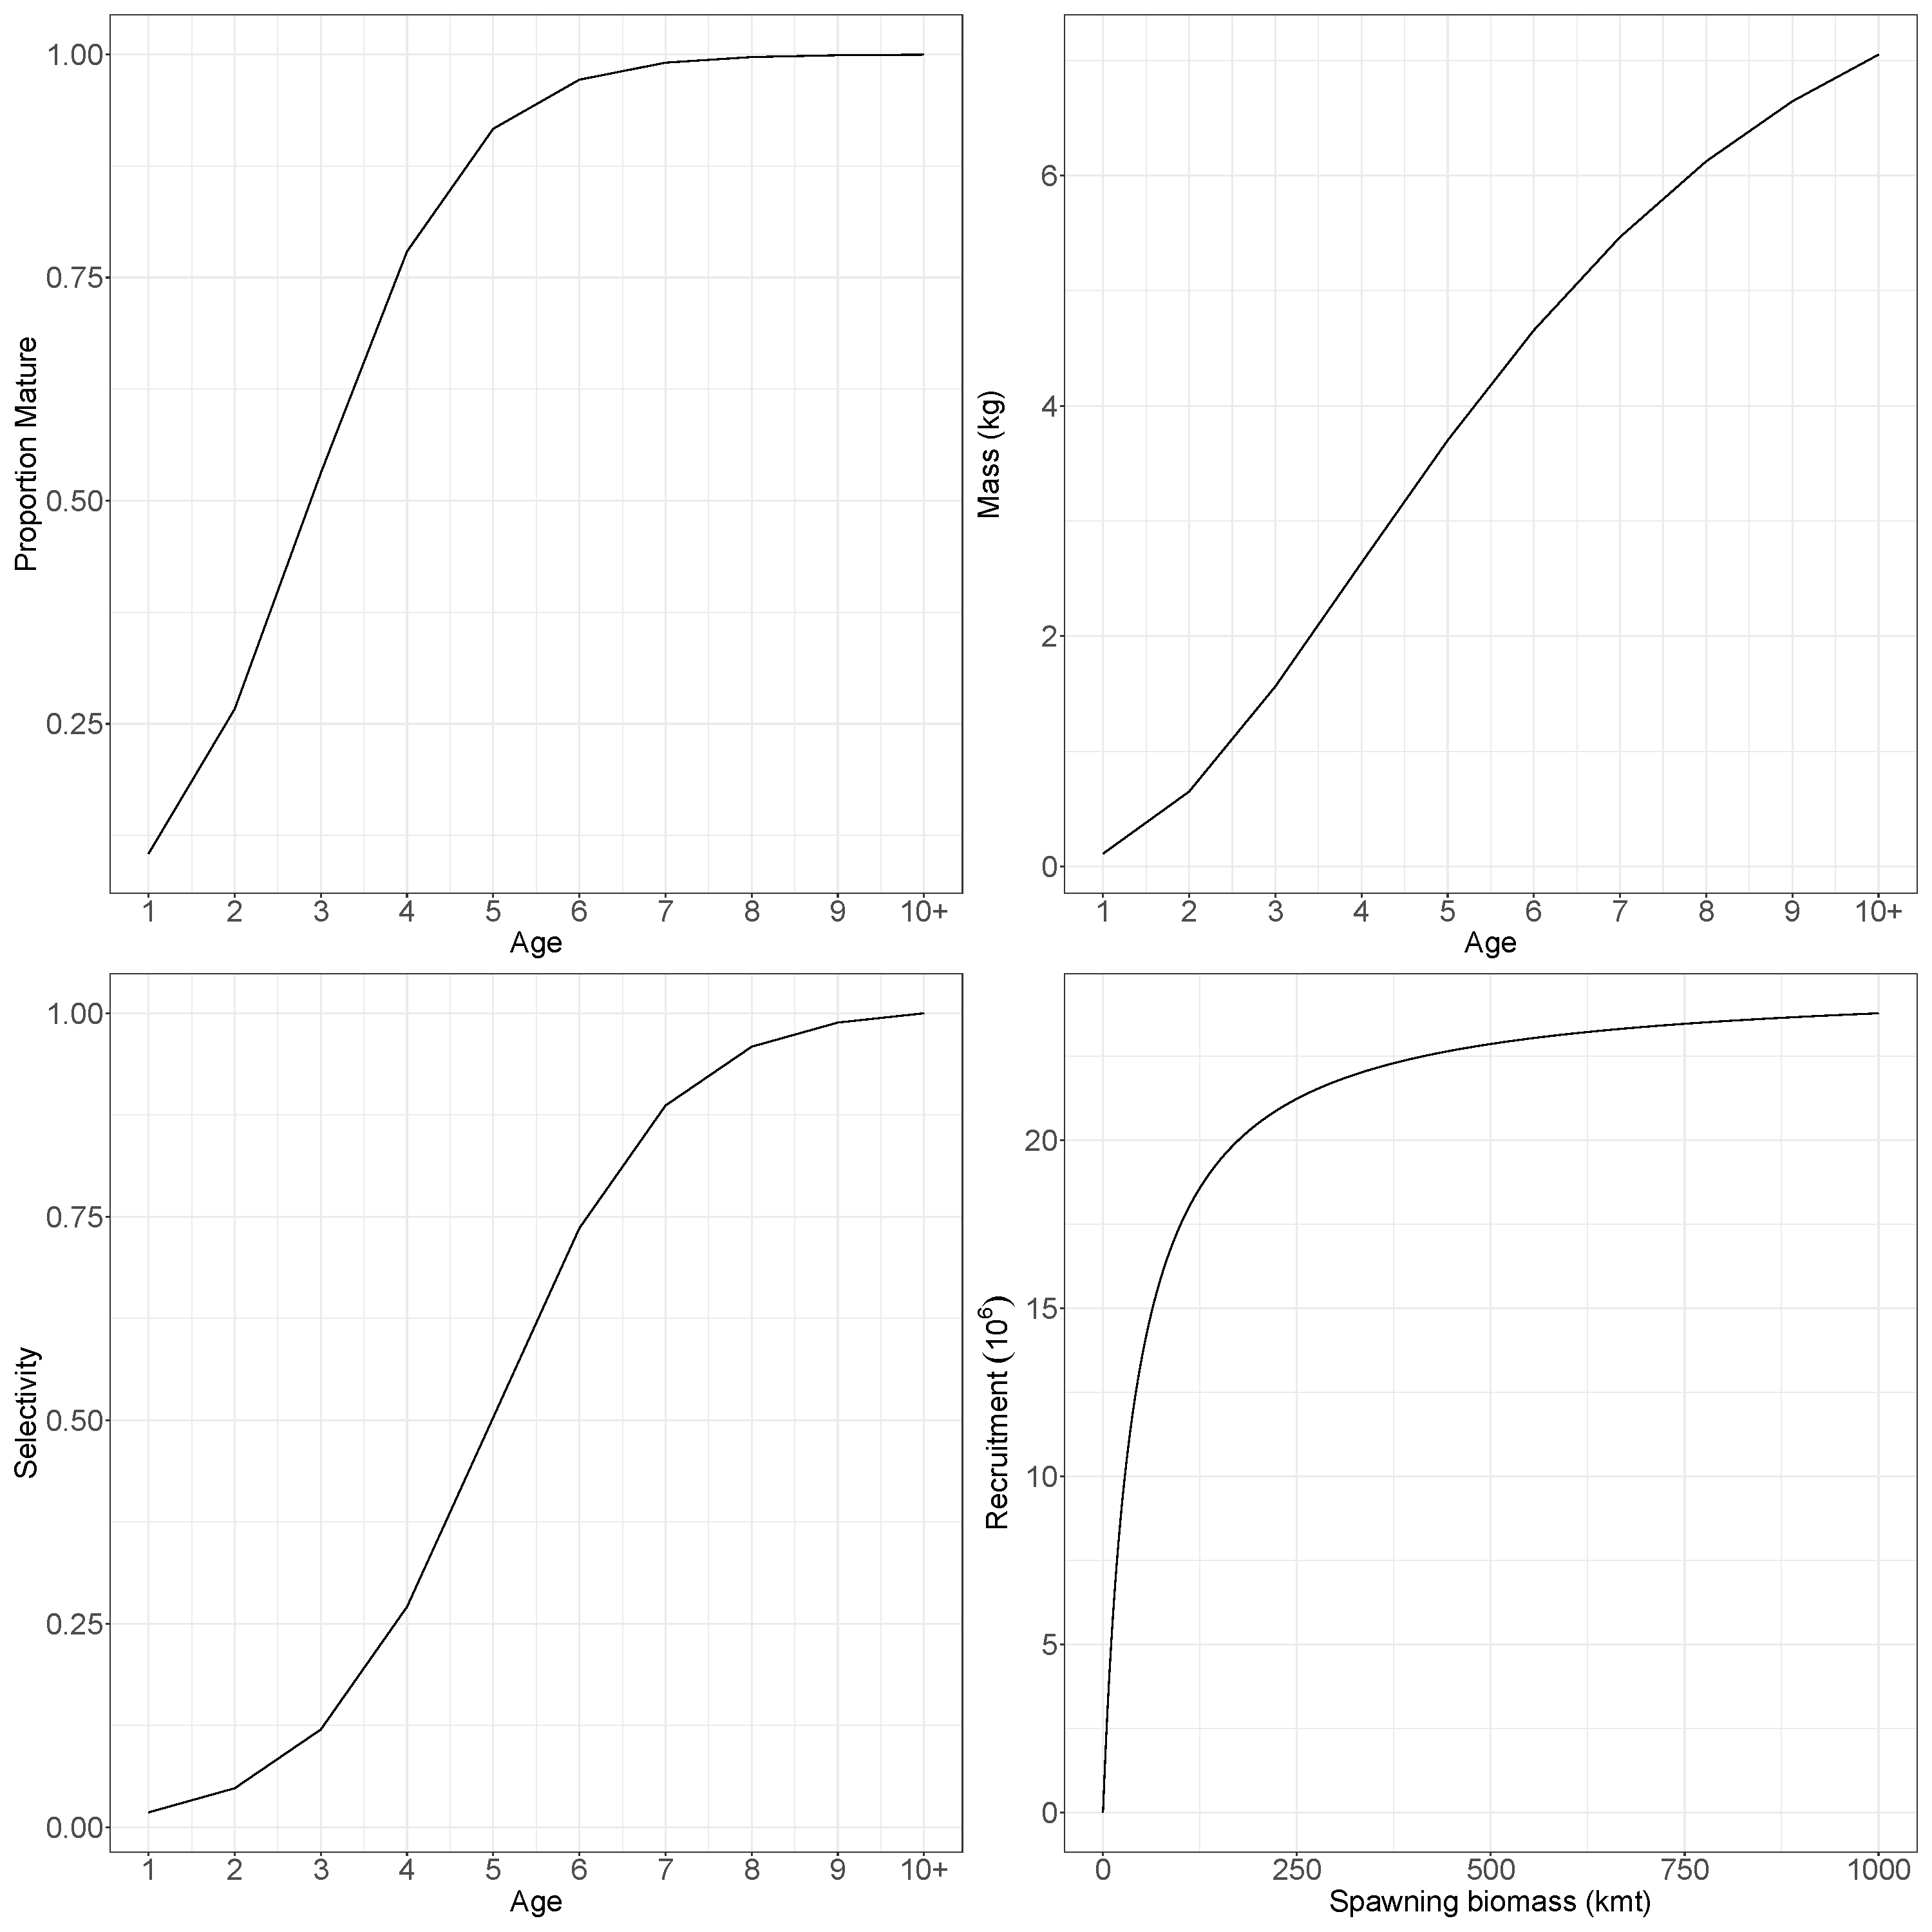
\includegraphics[width = \textwidth]{om_input_plots_figure}
\end{center}
\caption{The proportion mature at age, weight at age, fleet and index selectivity at age, and Beverton-Holt stock recruit relationship assumed for the population in all operating models. For operating models with random effects on fleet selectivity, this represents the selectivity at the mean of the random effects.}\label{om_inputs_fig}
\end{figure}

\clearpage

\begin{landscape}
\begin{figure}
\begin{center}
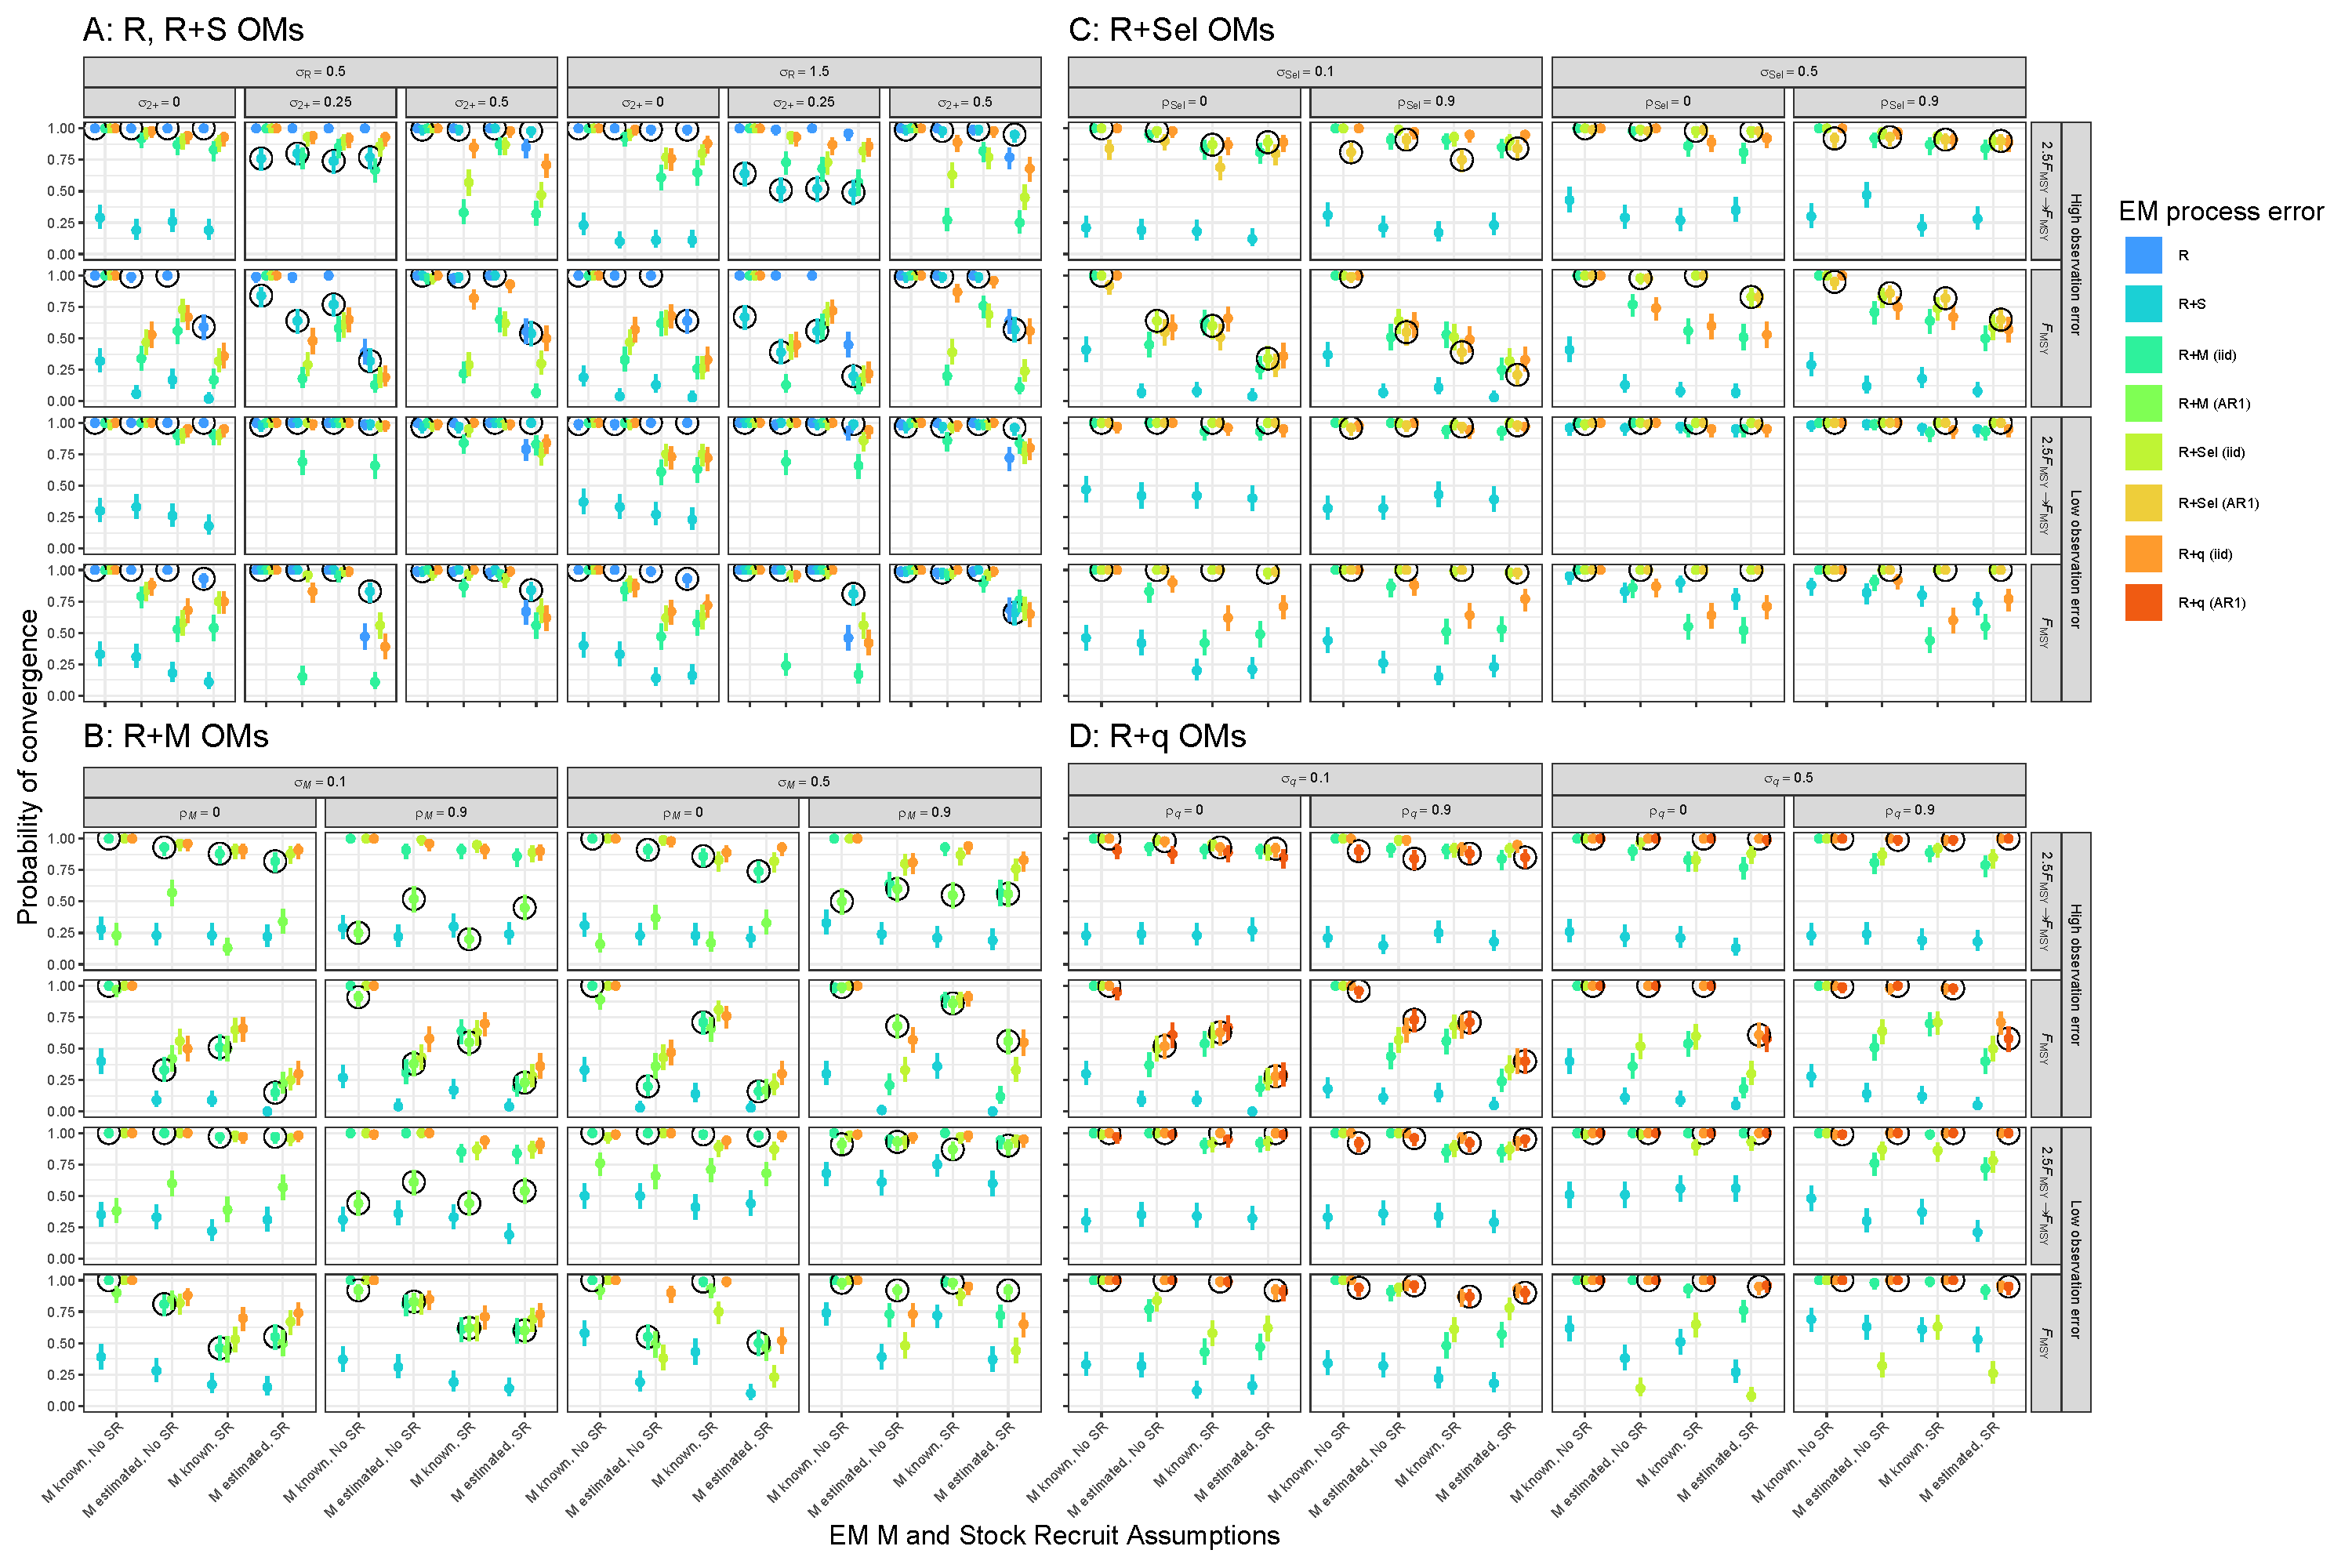
\includegraphics{type_4_convergence_plots}
\end{center}
\caption{Estimated probability of fits providing hessian-based standard errors for EMs assuming alternative process error (colored points and lines), and median natural mortality (estimated or known) and Beverton-Holt stock recruit functions (estimated or not; along x-axis) when fitted to operating models that have R and R+S (A), R+Sel (B), R+M (C), or R+q (D) process error structures. Circled values indicate results where the EM process error structure matches that of the operating model and vertical lines represent 95\% confidence intervals.}\label{hessian_SE_convergence}
\end{figure}
\end{landscape}

\clearpage

\begin{landscape}
\begin{figure}
\begin{center}
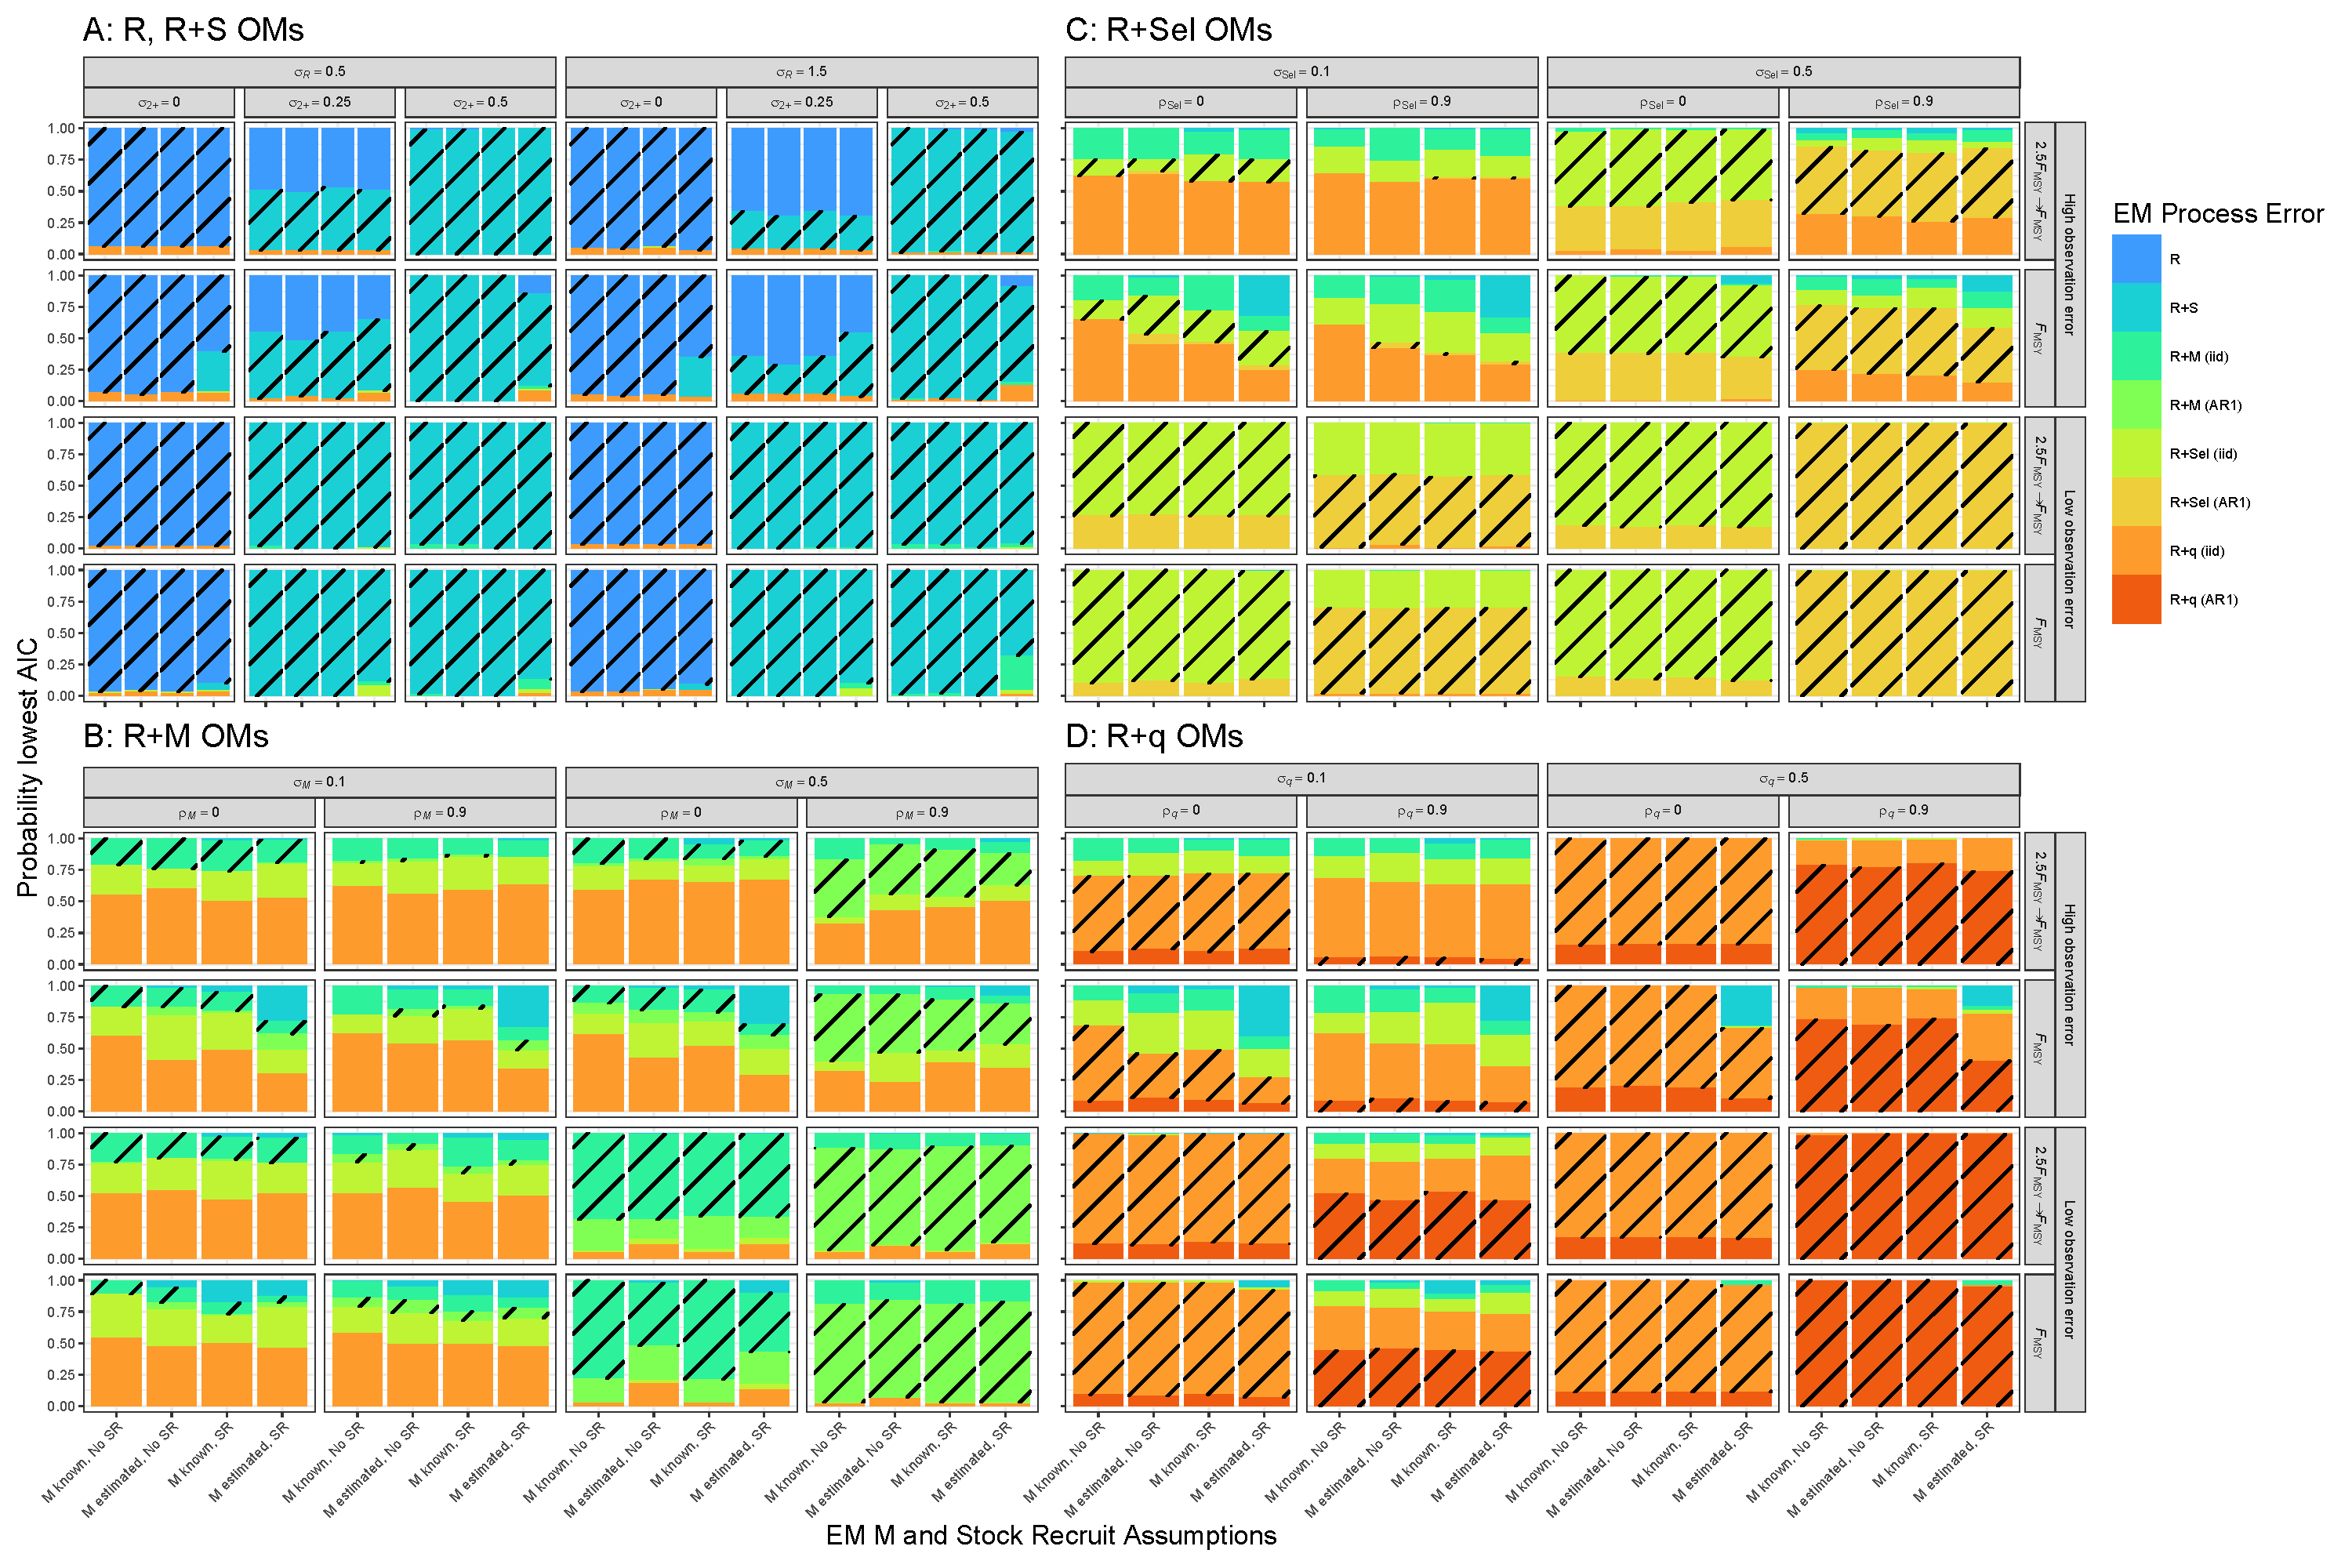
\includegraphics{pe_aic_plots}
\end{center}
\caption{Estimated probability of lowest AIC for EMs assuming alternative process error structures (colored bars) conditional on alternative assumptions for median natural mortality (estimated or known) and Beverton-Holt stock recruit functions (estimated or not; along x-axis) when fitted to operating models that have R and R+S (A), R+Sel (B), R+M (C), or R+q (D) process error structures. Striped bars indicate results where the EM process error structure matches that of the operating model.}\label{pe_aic}
\end{figure}
\end{landscape}

\clearpage

\begin{landscape}
\begin{figure}
\begin{center}
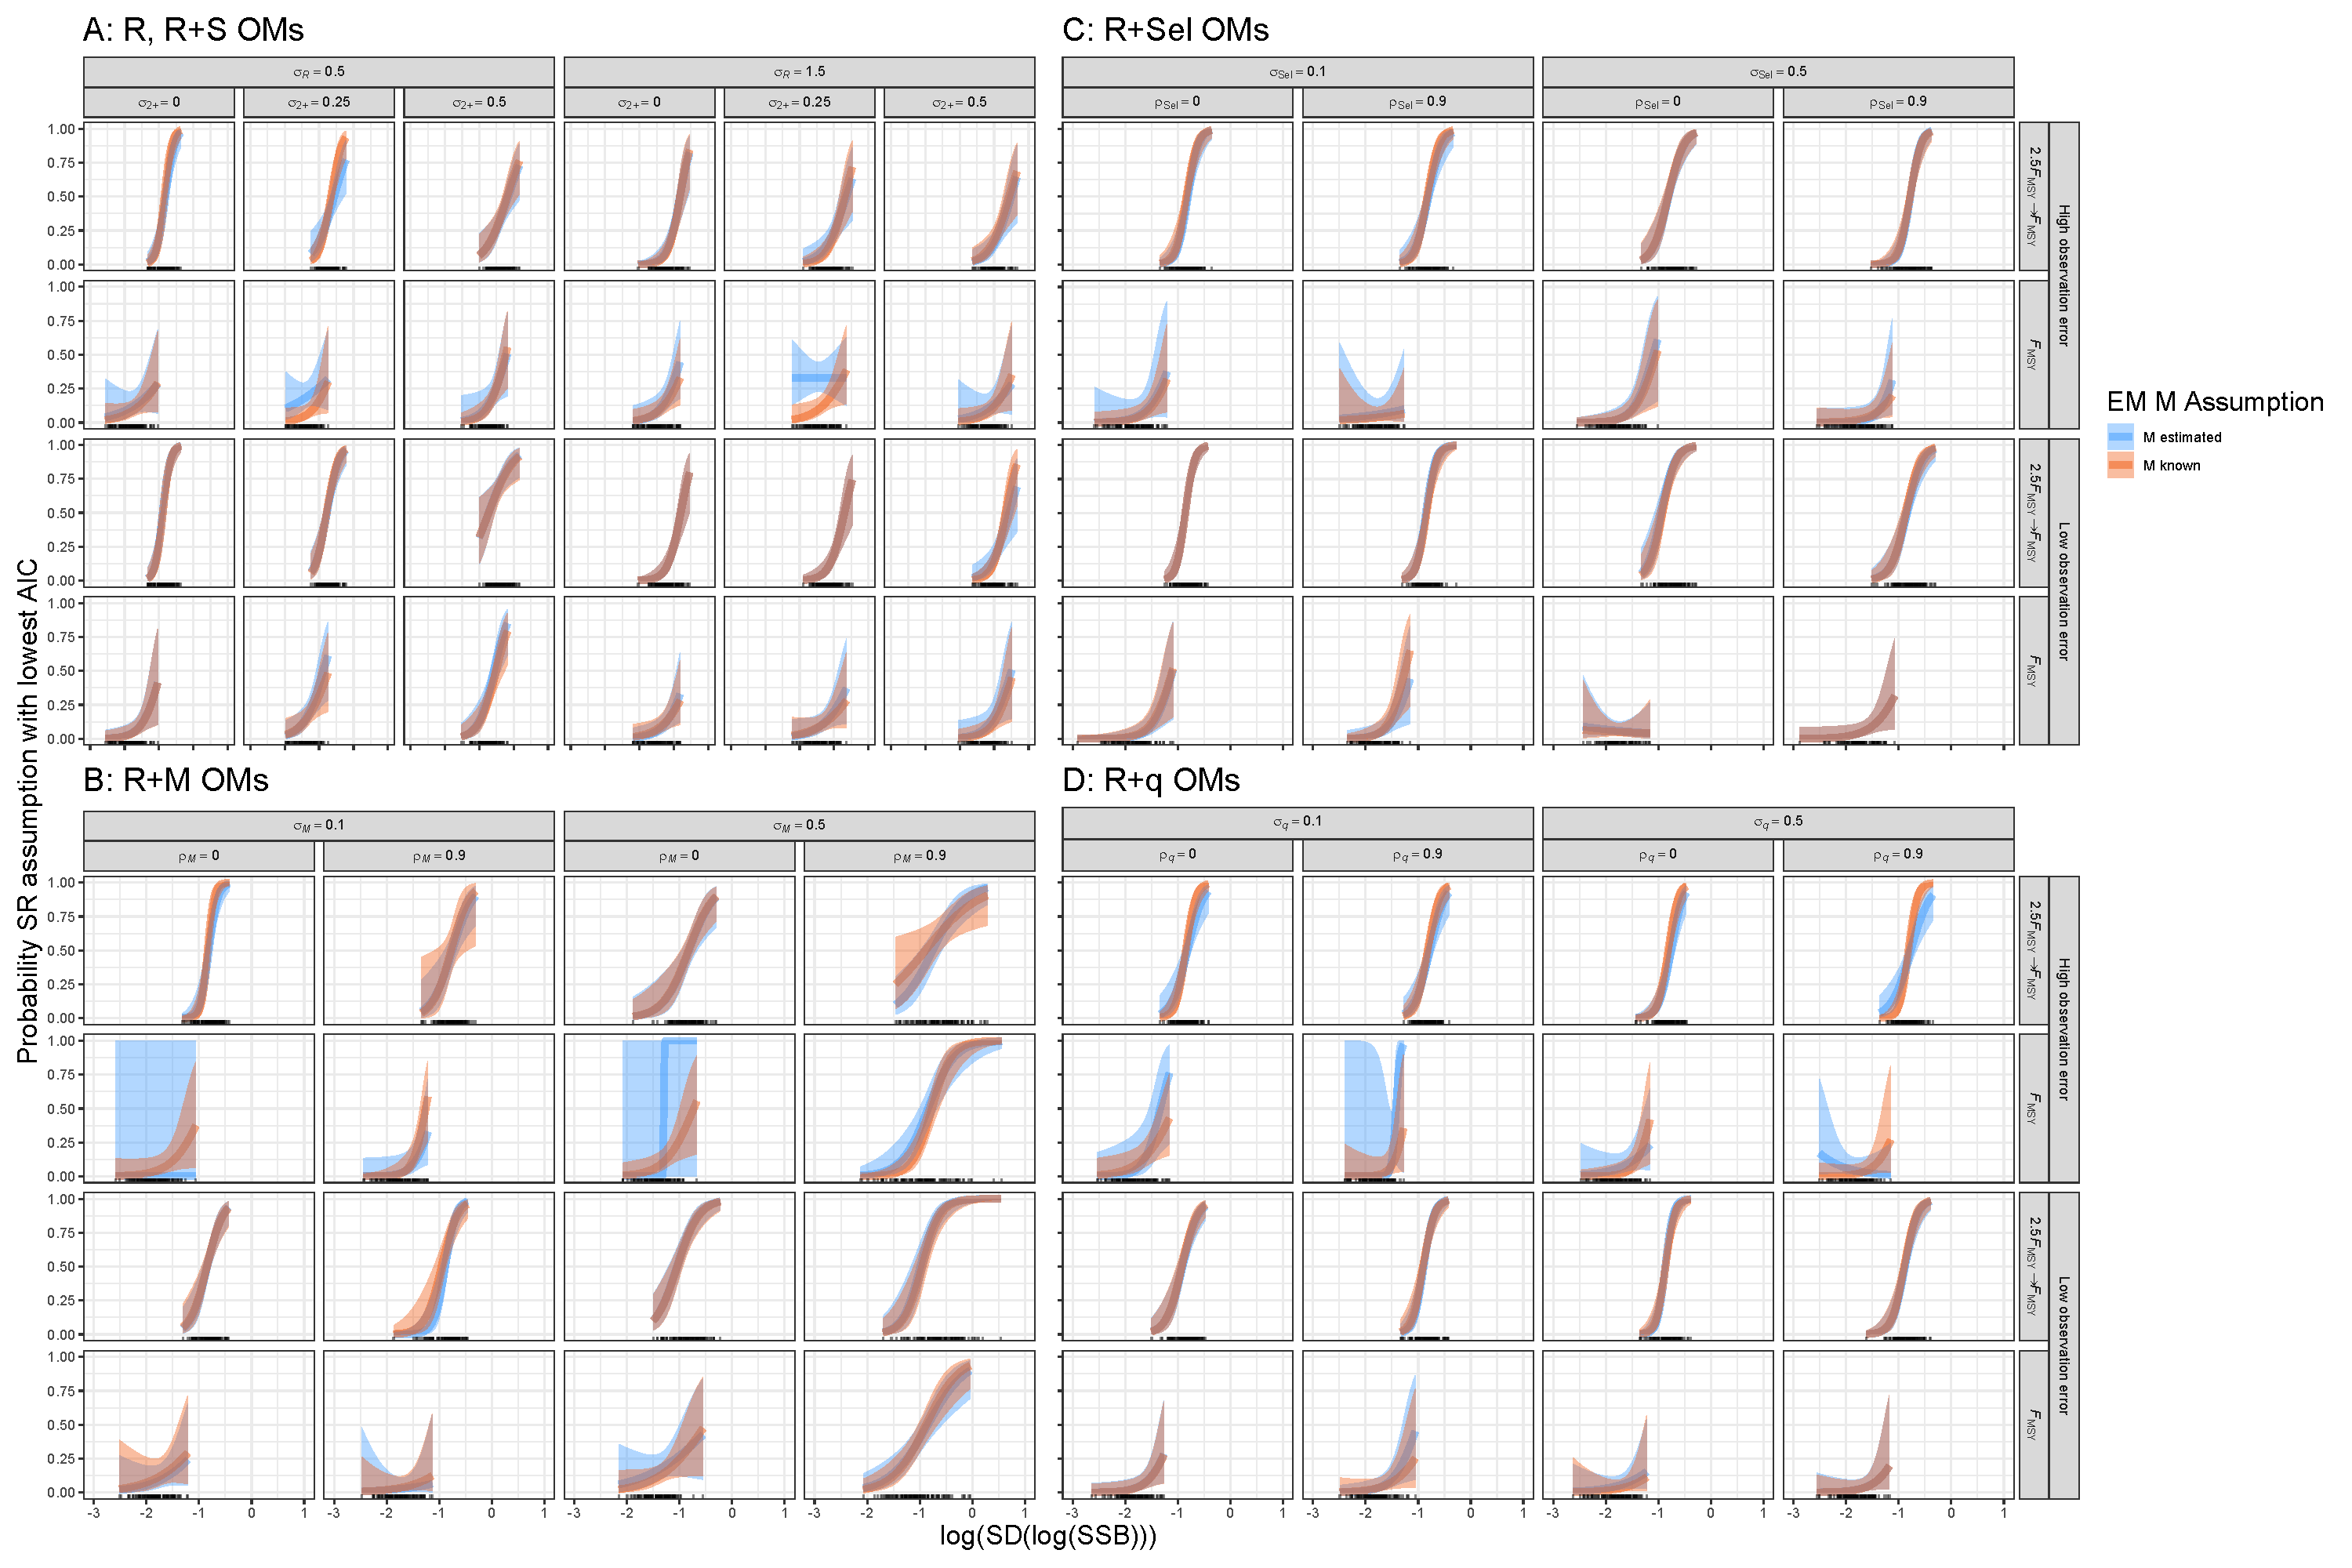
\includegraphics{sr_aic_plots}
\end{center}
\caption{Estimated probability of lowest AIC from logistic regression on the log-standard deviation of the true log(SSB) in each simulation for estimating model with Beverton-Holt stock recruit functions, rather than the otherwise equivalent EM without the stock recruit function. Results are conditional on alternative assumptions for median natural mortality (estimated or known) and on EMs having the correct process error structure: R and R+S (A), R+Sel (B), R+M (C), or R+q (D). Rug along x-axis denotes $SD(\log(SSB))$ values for each simulation amd polygons represent 95\% confidence intervals.}\label{sr_aic}
\end{figure}
\end{landscape}

\begin{landscape}
\begin{figure}
\begin{center}
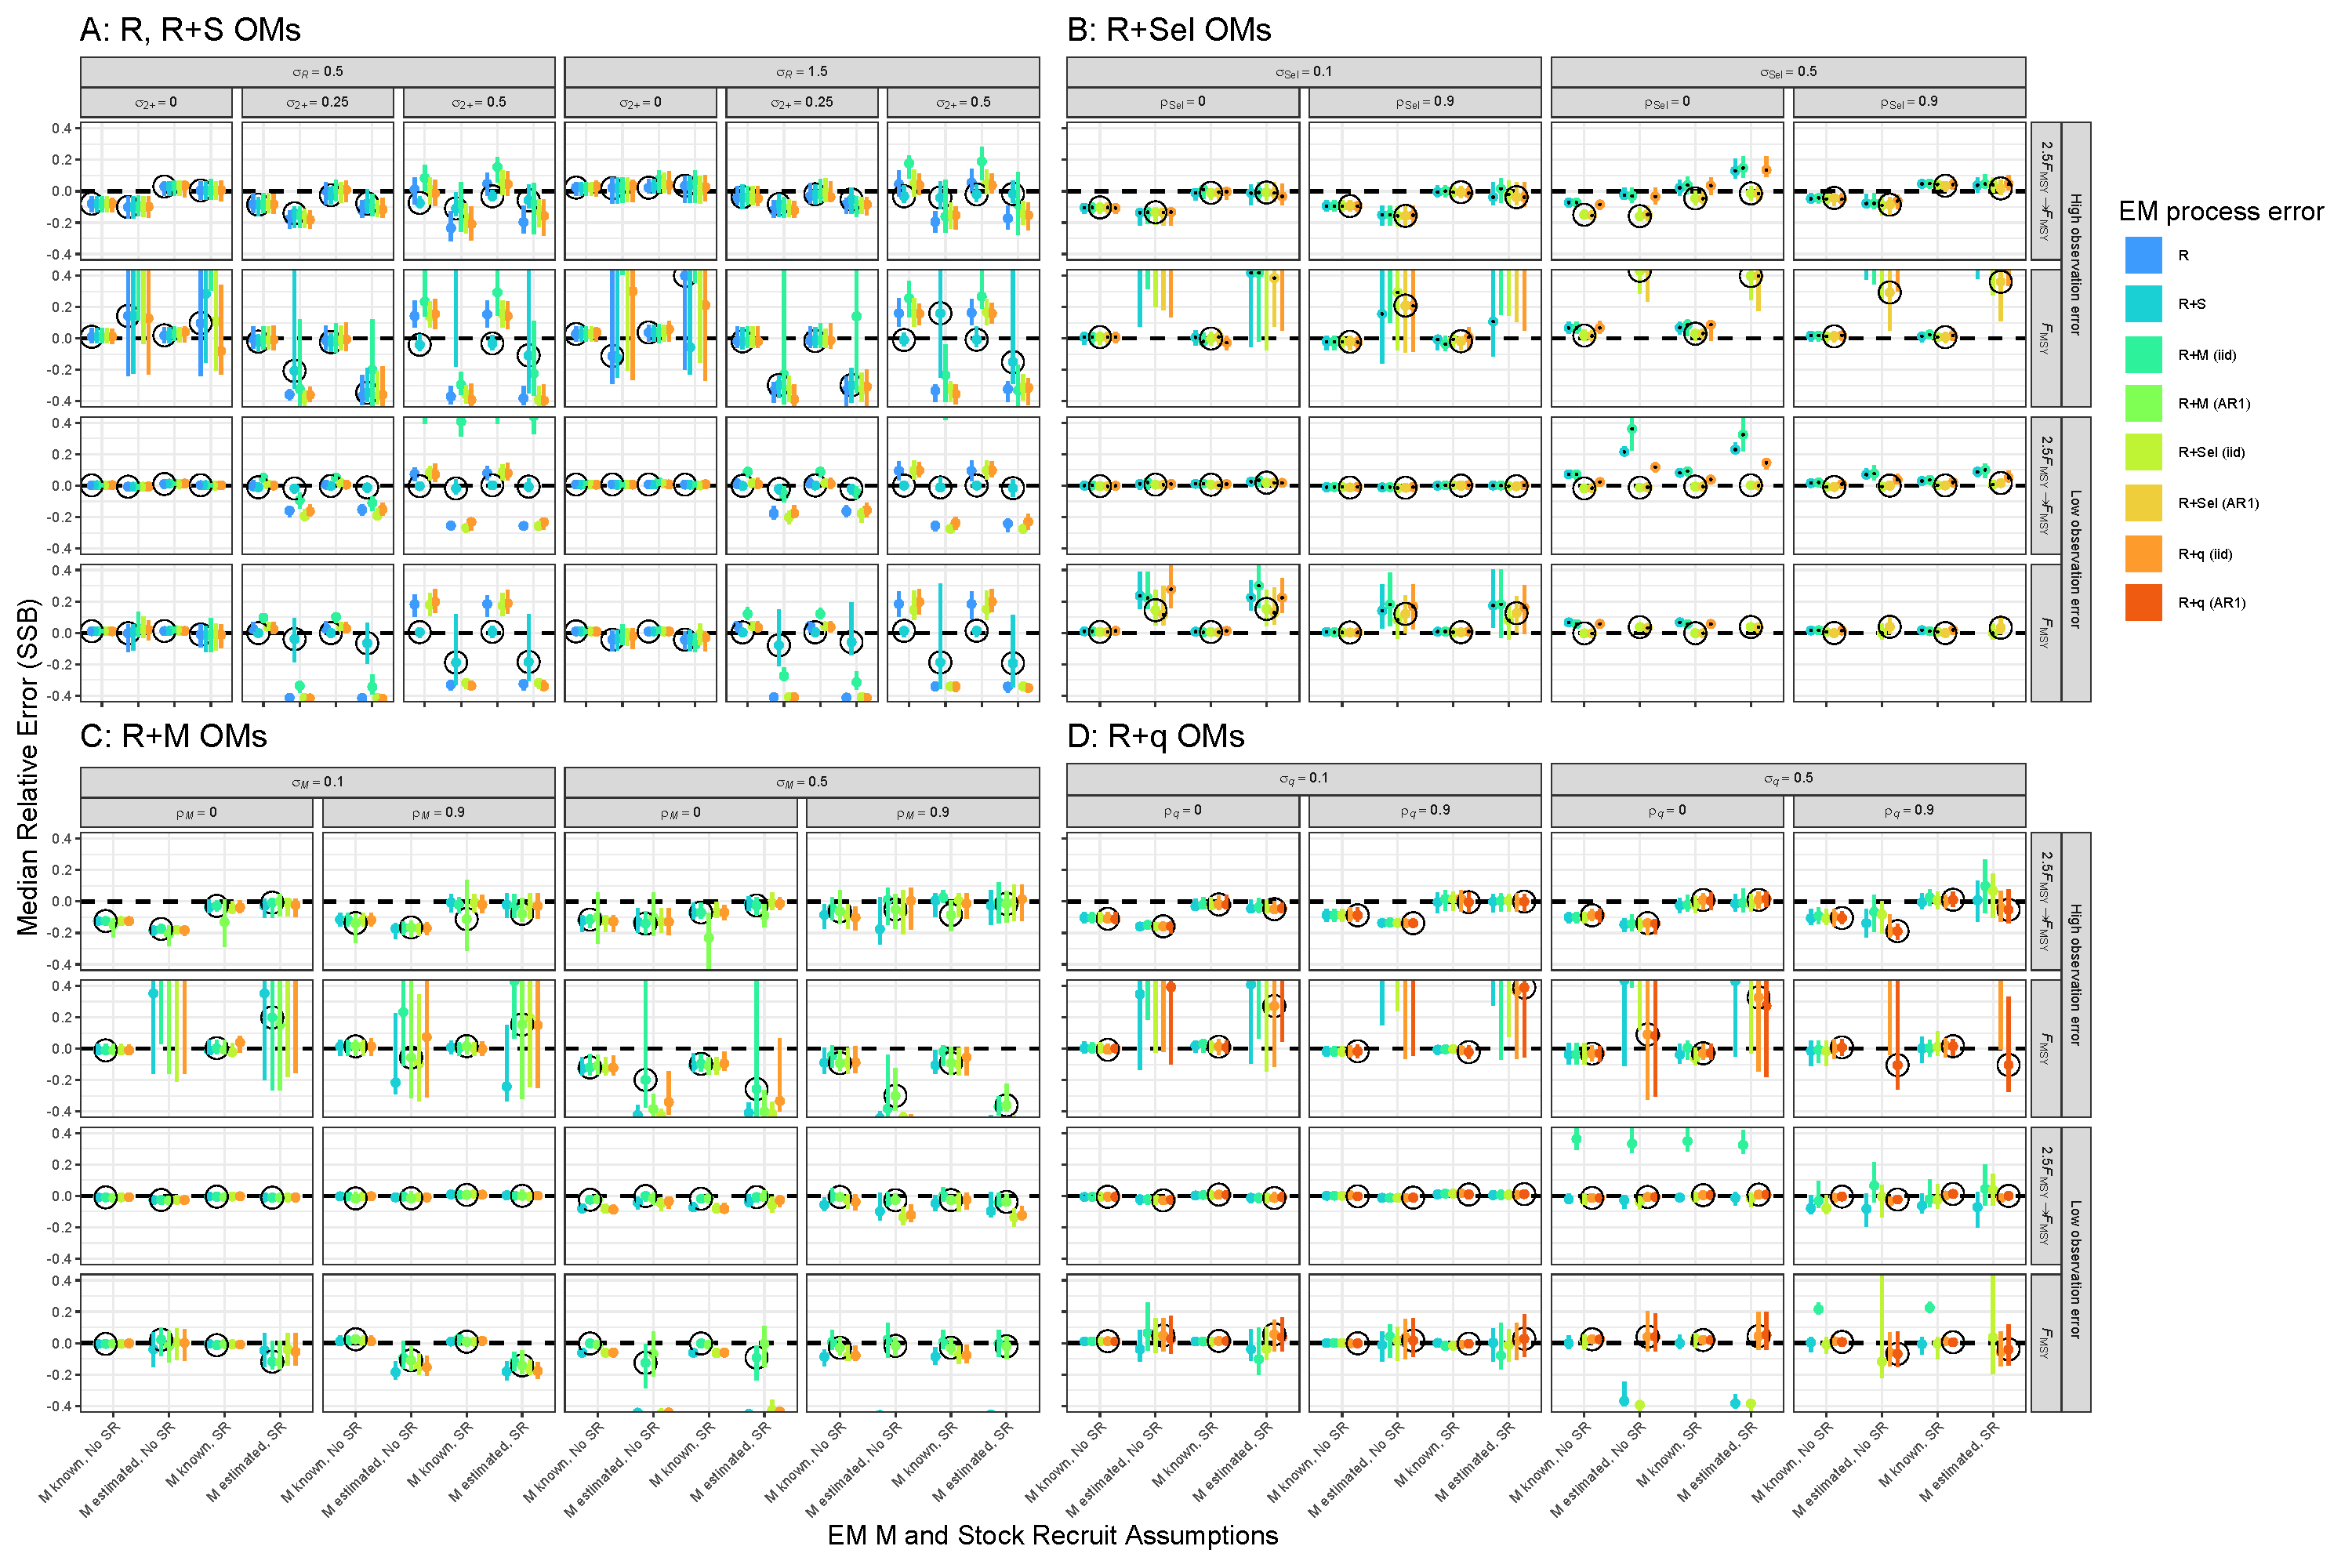
\includegraphics{term_SSB_bias_plots}
\end{center}
\caption{Median relative error of terminal year SSB for estimating models fitted to data sets simulated with alternative process error structures: R and R+S (A), R+Sel (B), R+M (C), or R+q (D).  Diamond shaped points denote results where the EM process error assumption matches that of the operating model. Circled values indicate results where the EM process error structure matches that of the operating model and vertical lines represent 95\% confidence intervals.}\label{SSB_rel_error}
\end{figure}
\end{landscape}

\begin{landscape}
\begin{figure}
\begin{center}
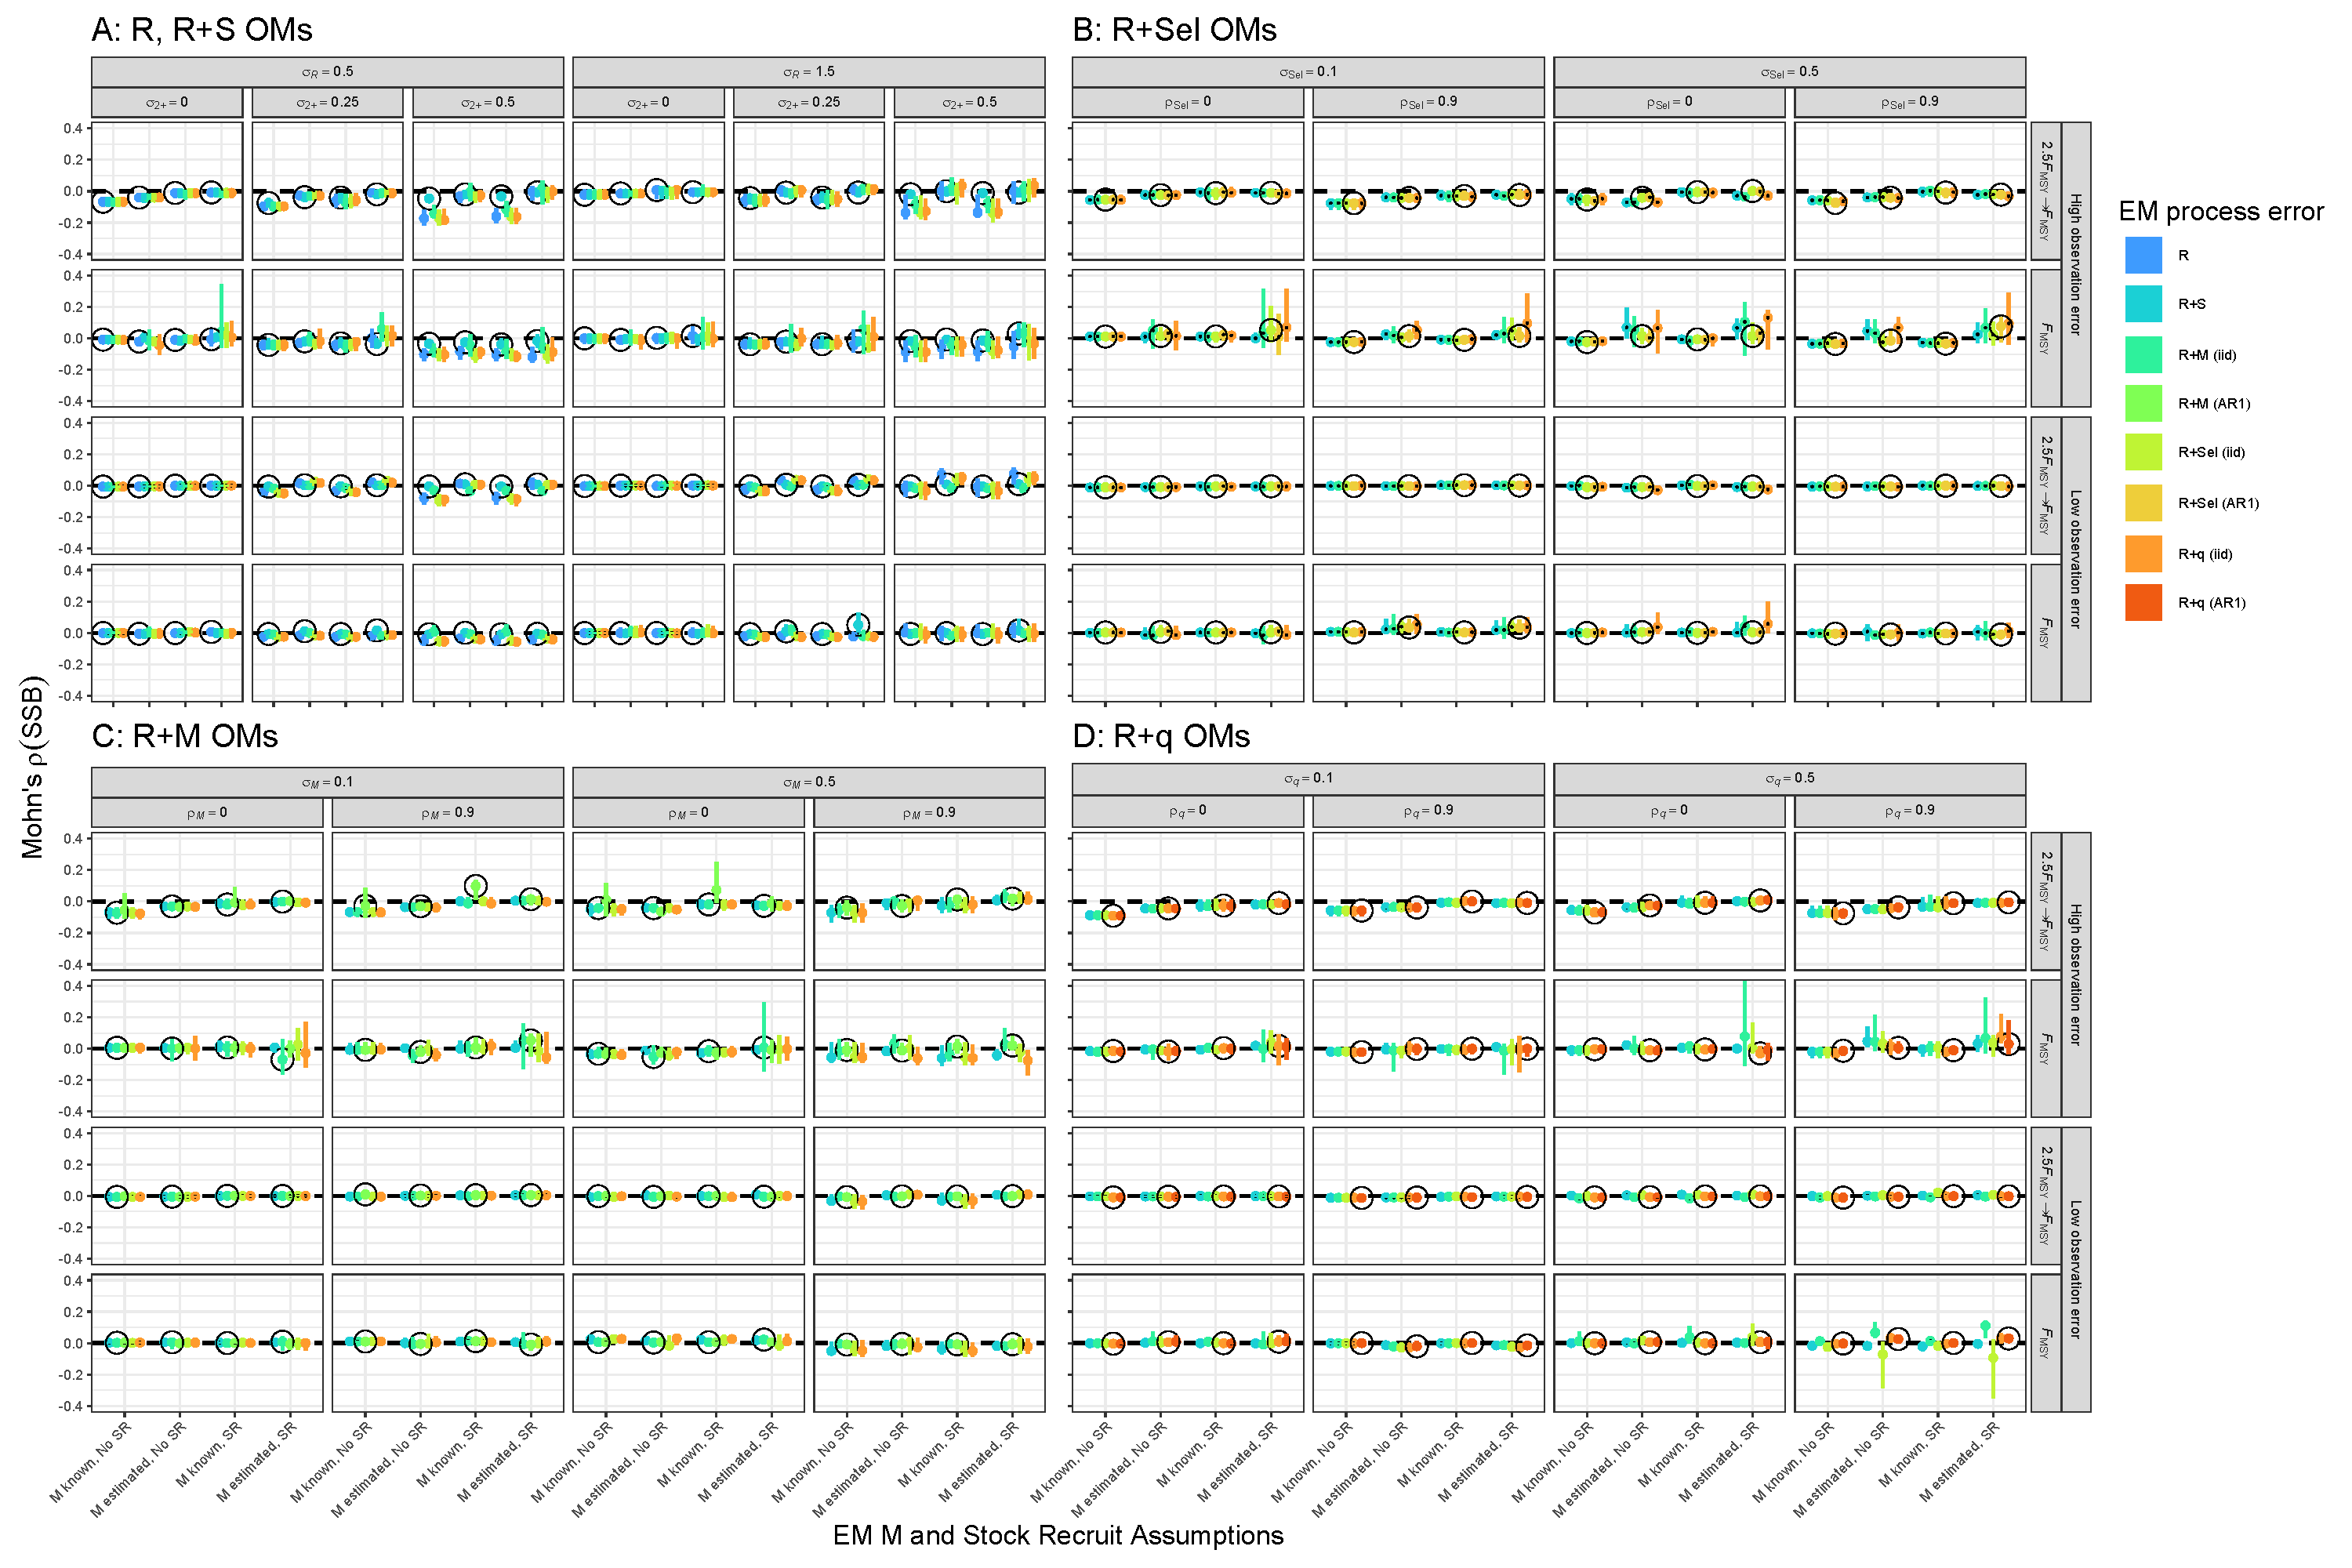
\includegraphics{mohns_rho_ssb_plots}
\end{center}
\caption{Median Mohn's rho for SSB for estimating models fitted to data sets simulated with alternative process error structures: R and R+S (A), R+Sel (B), R+M (C), or R+q (D). Circled values indicate results where the EM process error structure matches that of the operating model and vertical lines represent 95\% confidence intervals.}\label{mohns_rho_ssb}
\end{figure}
\end{landscape}

\pagebreak

\setcounter{figure}{0}
\renewcommand\thefigure{S\arabic{figure}}

\setcounter{table}{0}
\renewcommand\thetable{S\arabic{table}}

\hypertarget{supplementary-materials}{%
\section*{Supplementary Materials}\label{supplementary-materials}}
\addcontentsline{toc}{section}{Supplementary Materials}

\begin{landscape}
\begin{table}
\caption{Distinguishing characteristics of the operating models with random effects on survival. Standard deviations (SD) are for log-normal distributed indices and logistic normal distributed age composition observations (fleet and indices). Fishing mortality changes after year 20 (of 40) for fishing histories where fishing mortality is not constant.}\label{naa_om_table}
{\footnotesize \begin{center}
\begin{tabular}{rrrrr}
\hline\hline
\multicolumn{1}{c}{Model}&\multicolumn{1}{c}{$\sigma_R$}&\multicolumn{1}{c}{$\sigma_{2+}$}&\multicolumn{1}{c}{Fishing History}&\multicolumn{1}{c}{Observation Uncertainty}\tabularnewline
\hline
NAA_1&$0.5$&$$&$2.5 F_{\text{MSY}} \rightarrow F_{\text{MSY}}$&Index sigma (log scale) = 0.1, Age composition sigma (logistic normal) = 0.3\tabularnewline
NAA_2&$1.5$&$$&$2.5 F_{\text{MSY}} \rightarrow F_{\text{MSY}}$&Index sigma (log scale) = 0.1, Age composition sigma (logistic normal) = 0.3\tabularnewline
NAA_3&$0.5$&$0.25$&$2.5 F_{\text{MSY}} \rightarrow F_{\text{MSY}}$&Index sigma (log scale) = 0.1, Age composition sigma (logistic normal) = 0.3\tabularnewline
NAA_4&$1.5$&$0.25$&$2.5 F_{\text{MSY}} \rightarrow F_{\text{MSY}}$&Index sigma (log scale) = 0.1, Age composition sigma (logistic normal) = 0.3\tabularnewline
NAA_5&$0.5$&$0.50$&$2.5 F_{\text{MSY}} \rightarrow F_{\text{MSY}}$&Index sigma (log scale) = 0.1, Age composition sigma (logistic normal) = 0.3\tabularnewline
NAA_6&$1.5$&$0.50$&$2.5 F_{\text{MSY}} \rightarrow F_{\text{MSY}}$&Index sigma (log scale) = 0.1, Age composition sigma (logistic normal) = 0.3\tabularnewline
NAA_7&$0.5$&$$&F_{\text{MSY}}&Index sigma (log scale) = 0.1, Age composition sigma (logistic normal) = 0.3\tabularnewline
NAA_8&$1.5$&$$&F_{\text{MSY}}&Index sigma (log scale) = 0.1, Age composition sigma (logistic normal) = 0.3\tabularnewline
NAA_9&$0.5$&$0.25$&F_{\text{MSY}}&Index sigma (log scale) = 0.1, Age composition sigma (logistic normal) = 0.3\tabularnewline
NAA_10&$1.5$&$0.25$&F_{\text{MSY}}&Index sigma (log scale) = 0.1, Age composition sigma (logistic normal) = 0.3\tabularnewline
NAA_11&$0.5$&$0.50$&F_{\text{MSY}}&Index sigma (log scale) = 0.1, Age composition sigma (logistic normal) = 0.3\tabularnewline
NAA_12&$1.5$&$0.50$&F_{\text{MSY}}&Index sigma (log scale) = 0.1, Age composition sigma (logistic normal) = 0.3\tabularnewline
NAA_13&$0.5$&$$&$2.5 F_{\text{MSY}} \rightarrow F_{\text{MSY}}$&Index sigma (log scale) = 0.4, Age composition sigma (logistic normal) = 1.5\tabularnewline
NAA_14&$1.5$&$$&$2.5 F_{\text{MSY}} \rightarrow F_{\text{MSY}}$&Index sigma (log scale) = 0.4, Age composition sigma (logistic normal) = 1.5\tabularnewline
NAA_15&$0.5$&$0.25$&$2.5 F_{\text{MSY}} \rightarrow F_{\text{MSY}}$&Index sigma (log scale) = 0.4, Age composition sigma (logistic normal) = 1.5\tabularnewline
NAA_16&$1.5$&$0.25$&$2.5 F_{\text{MSY}} \rightarrow F_{\text{MSY}}$&Index sigma (log scale) = 0.4, Age composition sigma (logistic normal) = 1.5\tabularnewline
NAA_17&$0.5$&$0.50$&$2.5 F_{\text{MSY}} \rightarrow F_{\text{MSY}}$&Index sigma (log scale) = 0.4, Age composition sigma (logistic normal) = 1.5\tabularnewline
NAA_18&$1.5$&$0.50$&$2.5 F_{\text{MSY}} \rightarrow F_{\text{MSY}}$&Index sigma (log scale) = 0.4, Age composition sigma (logistic normal) = 1.5\tabularnewline
NAA_19&$0.5$&$$&F_{\text{MSY}}&Index sigma (log scale) = 0.4, Age composition sigma (logistic normal) = 1.5\tabularnewline
NAA_20&$1.5$&$$&F_{\text{MSY}}&Index sigma (log scale) = 0.4, Age composition sigma (logistic normal) = 1.5\tabularnewline
NAA_21&$0.5$&$0.25$&F_{\text{MSY}}&Index sigma (log scale) = 0.4, Age composition sigma (logistic normal) = 1.5\tabularnewline
NAA_22&$1.5$&$0.25$&F_{\text{MSY}}&Index sigma (log scale) = 0.4, Age composition sigma (logistic normal) = 1.5\tabularnewline
NAA_23&$0.5$&$0.50$&F_{\text{MSY}}&Index sigma (log scale) = 0.4, Age composition sigma (logistic normal) = 1.5\tabularnewline
NAA_24&$1.5$&$0.50$&F_{\text{MSY}}&Index sigma (log scale) = 0.4, Age composition sigma (logistic normal) = 1.5\tabularnewline
\hline
\end{tabular}\end{center}
}
\end{table}
\end{landscape}

\begin{landscape}
\begin{table}
\caption{Distinguishing characteristics of the operating models with random effects on natural mortality. Standard deviations (SD) are for log-normal distributed indices and logistic normal distributed age composition observations (fleet and indices). Fishing mortality changes after year 20 (of 40) for fishing histories where fishing mortality is not constant. For AR1 process errors, $\sigma$ is defined for the marginal distribution of the processes.}\label{M_om_table}
{\begin{center}
\begin{tabular}{rrrrrr}
\hline\hline
\multicolumn{1}{c}{Model}&\multicolumn{1}{c}{$\sigma_R$}&\multicolumn{1}{c}{$\sigma_{M}$}&\multicolumn{1}{c}{$\rho_{M}$}&\multicolumn{1}{c}{Fishing History}&\multicolumn{1}{c}{Observation Uncertainty}\tabularnewline
\hline
$M_{1}$&$0.5$&$0.1$&$0.0$&$2.5 F_{\text{MSY}} \rightarrow F_{\text{MSY}}$&Index SD = 0.1, Age composition SD = 0.3\tabularnewline
$M_{2}$&$0.5$&$0.5$&$0.0$&$2.5 F_{\text{MSY}} \rightarrow F_{\text{MSY}}$&Index SD = 0.1, Age composition SD = 0.3\tabularnewline
$M_{3}$&$0.5$&$0.1$&$0.9$&$2.5 F_{\text{MSY}} \rightarrow F_{\text{MSY}}$&Index SD = 0.1, Age composition SD = 0.3\tabularnewline
$M_{4}$&$0.5$&$0.5$&$0.9$&$2.5 F_{\text{MSY}} \rightarrow F_{\text{MSY}}$&Index SD = 0.1, Age composition SD = 0.3\tabularnewline
$M_{5}$&$0.5$&$0.1$&$0.0$&$F_{\text{MSY}}$&Index SD = 0.1, Age composition SD = 0.3\tabularnewline
$M_{6}$&$0.5$&$0.5$&$0.0$&$F_{\text{MSY}}$&Index SD = 0.1, Age composition SD = 0.3\tabularnewline
$M_{7}$&$0.5$&$0.1$&$0.9$&$F_{\text{MSY}}$&Index SD = 0.1, Age composition SD = 0.3\tabularnewline
$M_{8}$&$0.5$&$0.5$&$0.9$&$F_{\text{MSY}}$&Index SD = 0.1, Age composition SD = 0.3\tabularnewline
$M_{9}$&$0.5$&$0.1$&$0.0$&$2.5 F_{\text{MSY}} \rightarrow F_{\text{MSY}}$&Index SD = 0.4, Age composition SD = 1.5\tabularnewline
$M_{10}$&$0.5$&$0.5$&$0.0$&$2.5 F_{\text{MSY}} \rightarrow F_{\text{MSY}}$&Index SD = 0.4, Age composition SD = 1.5\tabularnewline
$M_{11}$&$0.5$&$0.1$&$0.9$&$2.5 F_{\text{MSY}} \rightarrow F_{\text{MSY}}$&Index SD = 0.4, Age composition SD = 1.5\tabularnewline
$M_{12}$&$0.5$&$0.5$&$0.9$&$2.5 F_{\text{MSY}} \rightarrow F_{\text{MSY}}$&Index SD = 0.4, Age composition SD = 1.5\tabularnewline
$M_{13}$&$0.5$&$0.1$&$0.0$&$F_{\text{MSY}}$&Index SD = 0.4, Age composition SD = 1.5\tabularnewline
$M_{14}$&$0.5$&$0.5$&$0.0$&$F_{\text{MSY}}$&Index SD = 0.4, Age composition SD = 1.5\tabularnewline
$M_{15}$&$0.5$&$0.1$&$0.9$&$F_{\text{MSY}}$&Index SD = 0.4, Age composition SD = 1.5\tabularnewline
$M_{16}$&$0.5$&$0.5$&$0.9$&$F_{\text{MSY}}$&Index SD = 0.4, Age composition SD = 1.5\tabularnewline
\hline
\end{tabular}\end{center}
}
\end{table}
\end{landscape}

\begin{landscape}
\begin{table}
\caption{Distinguishing characteristics of the operating models with random effects on selectivity. Standard deviations (SD) are for log-normal distributed indices and logistic normal distributed age composition observations (fleet and indices). Fishing mortality changes after year 20 (of 40) for fishing histories where fishing mortality is not constant. For AR1 process errors, $\sigma$ is defined for the marginal distribution of the processes.}\label{sel_om_table}
{\begin{center}
\begin{tabular}{rrrrrr}
\hline\hline
\multicolumn{1}{c}{Model}&\multicolumn{1}{c}{$\sigma_R$}&\multicolumn{1}{c}{$\sigma_{\text{Sel}}$}&\multicolumn{1}{c}{$\rho_{\text{Sel}}$}&\multicolumn{1}{c}{Fishing History}&\multicolumn{1}{c}{Observation Uncertainty}\tabularnewline
\hline
$\text{Sel}_{1}$&$0.5$&$0.1$&$0.0$&$2.5 F_{\text{MSY}} \rightarrow F_{\text{MSY}}$&Index SD = 0.1, Age composition SD = 0.3\tabularnewline
$\text{Sel}_{2}$&$0.5$&$0.5$&$0.0$&$2.5 F_{\text{MSY}} \rightarrow F_{\text{MSY}}$&Index SD = 0.1, Age composition SD = 0.3\tabularnewline
$\text{Sel}_{3}$&$0.5$&$0.1$&$0.9$&$2.5 F_{\text{MSY}} \rightarrow F_{\text{MSY}}$&Index SD = 0.1, Age composition SD = 0.3\tabularnewline
$\text{Sel}_{4}$&$0.5$&$0.5$&$0.9$&$2.5 F_{\text{MSY}} \rightarrow F_{\text{MSY}}$&Index SD = 0.1, Age composition SD = 0.3\tabularnewline
$\text{Sel}_{5}$&$0.5$&$0.1$&$0.0$&$F_{\text{MSY}}$&Index SD = 0.1, Age composition SD = 0.3\tabularnewline
$\text{Sel}_{6}$&$0.5$&$0.5$&$0.0$&$F_{\text{MSY}}$&Index SD = 0.1, Age composition SD = 0.3\tabularnewline
$\text{Sel}_{7}$&$0.5$&$0.1$&$0.9$&$F_{\text{MSY}}$&Index SD = 0.1, Age composition SD = 0.3\tabularnewline
$\text{Sel}_{8}$&$0.5$&$0.5$&$0.9$&$F_{\text{MSY}}$&Index SD = 0.1, Age composition SD = 0.3\tabularnewline
$\text{Sel}_{9}$&$0.5$&$0.1$&$0.0$&$2.5 F_{\text{MSY}} \rightarrow F_{\text{MSY}}$&Index SD = 0.4, Age composition SD = 1.5\tabularnewline
$\text{Sel}_{10}$&$0.5$&$0.5$&$0.0$&$2.5 F_{\text{MSY}} \rightarrow F_{\text{MSY}}$&Index SD = 0.4, Age composition SD = 1.5\tabularnewline
$\text{Sel}_{11}$&$0.5$&$0.1$&$0.9$&$2.5 F_{\text{MSY}} \rightarrow F_{\text{MSY}}$&Index SD = 0.4, Age composition SD = 1.5\tabularnewline
$\text{Sel}_{12}$&$0.5$&$0.5$&$0.9$&$2.5 F_{\text{MSY}} \rightarrow F_{\text{MSY}}$&Index SD = 0.4, Age composition SD = 1.5\tabularnewline
$\text{Sel}_{13}$&$0.5$&$0.1$&$0.0$&$F_{\text{MSY}}$&Index SD = 0.4, Age composition SD = 1.5\tabularnewline
$\text{Sel}_{14}$&$0.5$&$0.5$&$0.0$&$F_{\text{MSY}}$&Index SD = 0.4, Age composition SD = 1.5\tabularnewline
$\text{Sel}_{15}$&$0.5$&$0.1$&$0.9$&$F_{\text{MSY}}$&Index SD = 0.4, Age composition SD = 1.5\tabularnewline
$\text{Sel}_{16}$&$0.5$&$0.5$&$0.9$&$F_{\text{MSY}}$&Index SD = 0.4, Age composition SD = 1.5\tabularnewline
\hline
\end{tabular}\end{center}
}
\end{table}
\end{landscape}

\begin{landscape}
\begin{table}
\caption{Distinguishing characteristics of the operating models with random effects on catchability. Standard deviations (SD) are for log-normal distributed indices and logistic normal distributed age composition observations (fleet and indices). Fishing mortality changes after year 20 (of 40) for fishing histories where fishing mortality is not constant. For AR1 process errors, $\sigma$ is defined for the marginal distribution of the processes.}\label{q_om_table}
{\begin{center}
\begin{tabular}{rrrrrr}
\hline\hline
\multicolumn{1}{c}{Model}&\multicolumn{1}{c}{$\sigma_R$}&\multicolumn{1}{c}{$\sigma_{q}$}&\multicolumn{1}{c}{$\rho_{q}$}&\multicolumn{1}{c}{Fishing History}&\multicolumn{1}{c}{Observation Uncertainty}\tabularnewline
\hline
$q_{1}$&$0.5$&$0.1$&$0.0$&$2.5 F_{\text{MSY}} \rightarrow F_{\text{MSY}}$&Index SD = 0.1, Age composition SD = 0.3\tabularnewline
$q_{2}$&$0.5$&$0.5$&$0.0$&$2.5 F_{\text{MSY}} \rightarrow F_{\text{MSY}}$&Index SD = 0.1, Age composition SD = 0.3\tabularnewline
$q_{3}$&$0.5$&$0.1$&$0.9$&$2.5 F_{\text{MSY}} \rightarrow F_{\text{MSY}}$&Index SD = 0.1, Age composition SD = 0.3\tabularnewline
$q_{4}$&$0.5$&$0.5$&$0.9$&$2.5 F_{\text{MSY}} \rightarrow F_{\text{MSY}}$&Index SD = 0.1, Age composition SD = 0.3\tabularnewline
$q_{5}$&$0.5$&$0.1$&$0.0$&$F_{\text{MSY}}$&Index SD = 0.1, Age composition SD = 0.3\tabularnewline
$q_{6}$&$0.5$&$0.5$&$0.0$&$F_{\text{MSY}}$&Index SD = 0.1, Age composition SD = 0.3\tabularnewline
$q_{7}$&$0.5$&$0.1$&$0.9$&$F_{\text{MSY}}$&Index SD = 0.1, Age composition SD = 0.3\tabularnewline
$q_{8}$&$0.5$&$0.5$&$0.9$&$F_{\text{MSY}}$&Index SD = 0.1, Age composition SD = 0.3\tabularnewline
$q_{9}$&$0.5$&$0.1$&$0.0$&$2.5 F_{\text{MSY}} \rightarrow F_{\text{MSY}}$&Index SD = 0.4, Age composition SD = 1.5\tabularnewline
$q_{10}$&$0.5$&$0.5$&$0.0$&$2.5 F_{\text{MSY}} \rightarrow F_{\text{MSY}}$&Index SD = 0.4, Age composition SD = 1.5\tabularnewline
$q_{11}$&$0.5$&$0.1$&$0.9$&$2.5 F_{\text{MSY}} \rightarrow F_{\text{MSY}}$&Index SD = 0.4, Age composition SD = 1.5\tabularnewline
$q_{12}$&$0.5$&$0.5$&$0.9$&$2.5 F_{\text{MSY}} \rightarrow F_{\text{MSY}}$&Index SD = 0.4, Age composition SD = 1.5\tabularnewline
$q_{13}$&$0.5$&$0.1$&$0.0$&$F_{\text{MSY}}$&Index SD = 0.4, Age composition SD = 1.5\tabularnewline
$q_{14}$&$0.5$&$0.5$&$0.0$&$F_{\text{MSY}}$&Index SD = 0.4, Age composition SD = 1.5\tabularnewline
$q_{15}$&$0.5$&$0.1$&$0.9$&$F_{\text{MSY}}$&Index SD = 0.4, Age composition SD = 1.5\tabularnewline
$q_{16}$&$0.5$&$0.5$&$0.9$&$F_{\text{MSY}}$&Index SD = 0.4, Age composition SD = 1.5\tabularnewline
\hline
\end{tabular}\end{center}
}
\end{table}
\end{landscape}

\begin{table}
\caption{Distinguishing characteristics of the estimating models.}\label{em_table}
{\scriptsize \begin{center}
\begin{tabular}{rrrr}
\hline\hline
\multicolumn{1}{c}{Model}&\multicolumn{1}{c}{Recruitment model}&\multicolumn{1}{c}{Mean $M$}&\multicolumn{1}{c}{Process error assumption}\tabularnewline
\hline
EM$_{1}$&Mean recruitment&0.2&Recruitment ($\sigma_R$ estimated)\tabularnewline
EM$_{2}$&Beverton-Holt&0.2&Recruitment ($\sigma_R$ estimated)\tabularnewline
EM$_{3}$&Mean recruitment&Estimated&Recruitment ($\sigma_R$ estimated)\tabularnewline
EM$_{4}$&Beverton-Holt&Estimated&Recruitment ($\sigma_R$ estimated)\tabularnewline
EM$_{5}$&Mean recruitment&0.2&Recruitment and survival ($\sigma_R$, $\sigma_{2+}$ estimated)\tabularnewline
EM$_{6}$&Beverton-Holt&0.2&Recruitment and survival ($\sigma_R$, $\sigma_{2+}$ estimated)\tabularnewline
EM$_{7}$&Mean recruitment&Estimated&Recruitment and survival ($\sigma_R$, $\sigma_{2+}$ estimated)\tabularnewline
EM$_{8}$&Beverton-Holt&Estimated&Recruitment and survival ($\sigma_R$, $\sigma_{2+}$ estimated)\tabularnewline
EM$_{9}$&Mean recruitment&0.2&Recruitment and uncorrelated natural mortality ($\sigma_R$, $\sigma_{M}$ estimated, $\rho_{M} = 0$)\tabularnewline
EM$_{10}$&Beverton-Holt&0.2&Recruitment and uncorrelated natural mortality ($\sigma_R$, $\sigma_{M}$ estimated, $\rho_{M} = 0$)\tabularnewline
EM$_{11}$&Mean recruitment&Estimated&Recruitment and uncorrelated natural mortality ($\sigma_R$, $\sigma_{M}$ estimated, $\rho_{M} = 0$)\tabularnewline
EM$_{12}$&Beverton-Holt&Estimated&Recruitment and uncorrelated natural mortality ($\sigma_R$, $\sigma_{M}$ estimated, $\rho_{M} = 0$)\tabularnewline
EM$_{13}$&Mean recruitment&0.2&Recruitment and uncorrelated fleet selectivity ($\sigma_R$, $\sigma_{\text{Sel}}$ estimated, $\rho_{\text{Sel}} = 0$)\tabularnewline
EM$_{14}$&Beverton-Holt&0.2&Recruitment and uncorrelated fleet selectivity ($\sigma_R$, $\sigma_{\text{Sel}}$ estimated, $\rho_{\text{Sel}} = 0$)\tabularnewline
EM$_{15}$&Mean recruitment&Estimated&Recruitment and uncorrelated fleet selectivity ($\sigma_R$, $\sigma_{\text{Sel}}$ estimated, $\rho_{\text{Sel}} = 0$)\tabularnewline
EM$_{16}$&Beverton-Holt&Estimated&Recruitment and uncorrelated fleet selectivity ($\sigma_R$, $\sigma_{\text{Sel}}$ estimated, $\rho_{\text{Sel}} = 0$)\tabularnewline
EM$_{17}$&Mean recruitment&0.2&Recruitment and uncorrelated catchability (spring index) ($\sigma_R$, $\sigma_{q}$ estimated, $\rho_{q} = 0$)\tabularnewline
EM$_{18}$&Beverton-Holt&0.2&Recruitment and uncorrelated catchability (spring index) ($\sigma_R$, $\sigma_{q}$ estimated, $\rho_{q} = 0$)\tabularnewline
EM$_{19}$&Mean recruitment&Estimated&Recruitment and uncorrelated catchability (spring index) ($\sigma_R$, $\sigma_{q}$ estimated, $\rho_{q} = 0$)\tabularnewline
EM$_{20}$&Beverton-Holt&Estimated&Recruitment and uncorrelated catchability (spring index) ($\sigma_R$, $\sigma_{q}$ estimated, $\rho_{q} = 0$)\tabularnewline
EM$_{21}$&Mean recruitment&0.2&Recruitment and AR1 natural mortality ($\sigma_R$, $\sigma_{M}$, $\rho_{M}$ estimated)\tabularnewline
EM$_{22}$&Beverton-Holt&0.2&Recruitment and AR1 natural mortality ($\sigma_R$, $\sigma_{M}$, $\rho_{M}$ estimated)\tabularnewline
EM$_{23}$&Mean recruitment&Estimated&Recruitment and AR1 natural mortality ($\sigma_R$, $\sigma_{M}$, $\rho_{M}$ estimated)\tabularnewline
EM$_{24}$&Beverton-Holt&Estimated&Recruitment and AR1 natural mortality ($\sigma_R$, $\sigma_{M}$, $\rho_{M}$ estimated)\tabularnewline
EM$_{25}$&Mean recruitment&0.2&Recruitment and AR1 selectivity ($\sigma_R$, $\sigma_{\text{Sel}}$, $\rho_{\text{Sel}}$ estimated)\tabularnewline
EM$_{26}$&Beverton-Holt&0.2&Recruitment and AR1 selectivity ($\sigma_R$, $\sigma_{\text{Sel}}$, $\rho_{\text{Sel}}$ estimated)\tabularnewline
EM$_{27}$&Mean recruitment&Estimated&Recruitment and AR1 selectivity ($\sigma_R$, $\sigma_{\text{Sel}}$, $\rho_{\text{Sel}}$ estimated)\tabularnewline
EM$_{28}$&Beverton-Holt&Estimated&Recruitment and AR1 selectivity ($\sigma_R$, $\sigma_{\text{Sel}}$, $\rho_{\text{Sel}}$ estimated)\tabularnewline
EM$_{29}$&Mean recruitment&0.2&Recruitment and AR1 catchability (spring index) ($\sigma_R$, $\sigma_{q}$, $\rho_{q}$ estimated)\tabularnewline
EM$_{30}$&Beverton-Holt&0.2&Recruitment and AR1 catchability (spring index) ($\sigma_R$, $\sigma_{q}$, $\rho_{q}$ estimated)\tabularnewline
EM$_{31}$&Mean recruitment&Estimated&Recruitment and AR1 catchability (spring index) ($\sigma_R$, $\sigma_{q}$, $\rho_{q}$ estimated)\tabularnewline
EM$_{32}$&Beverton-Holt&Estimated&Recruitment and AR1 catchability (spring index) ($\sigma_R$, $\sigma_{q}$, $\rho_{q}$ estimated)\tabularnewline
\hline
\end{tabular}\end{center}
}
\end{table}

\clearpage

\begin{landscape}
\begin{figure}
\begin{center}
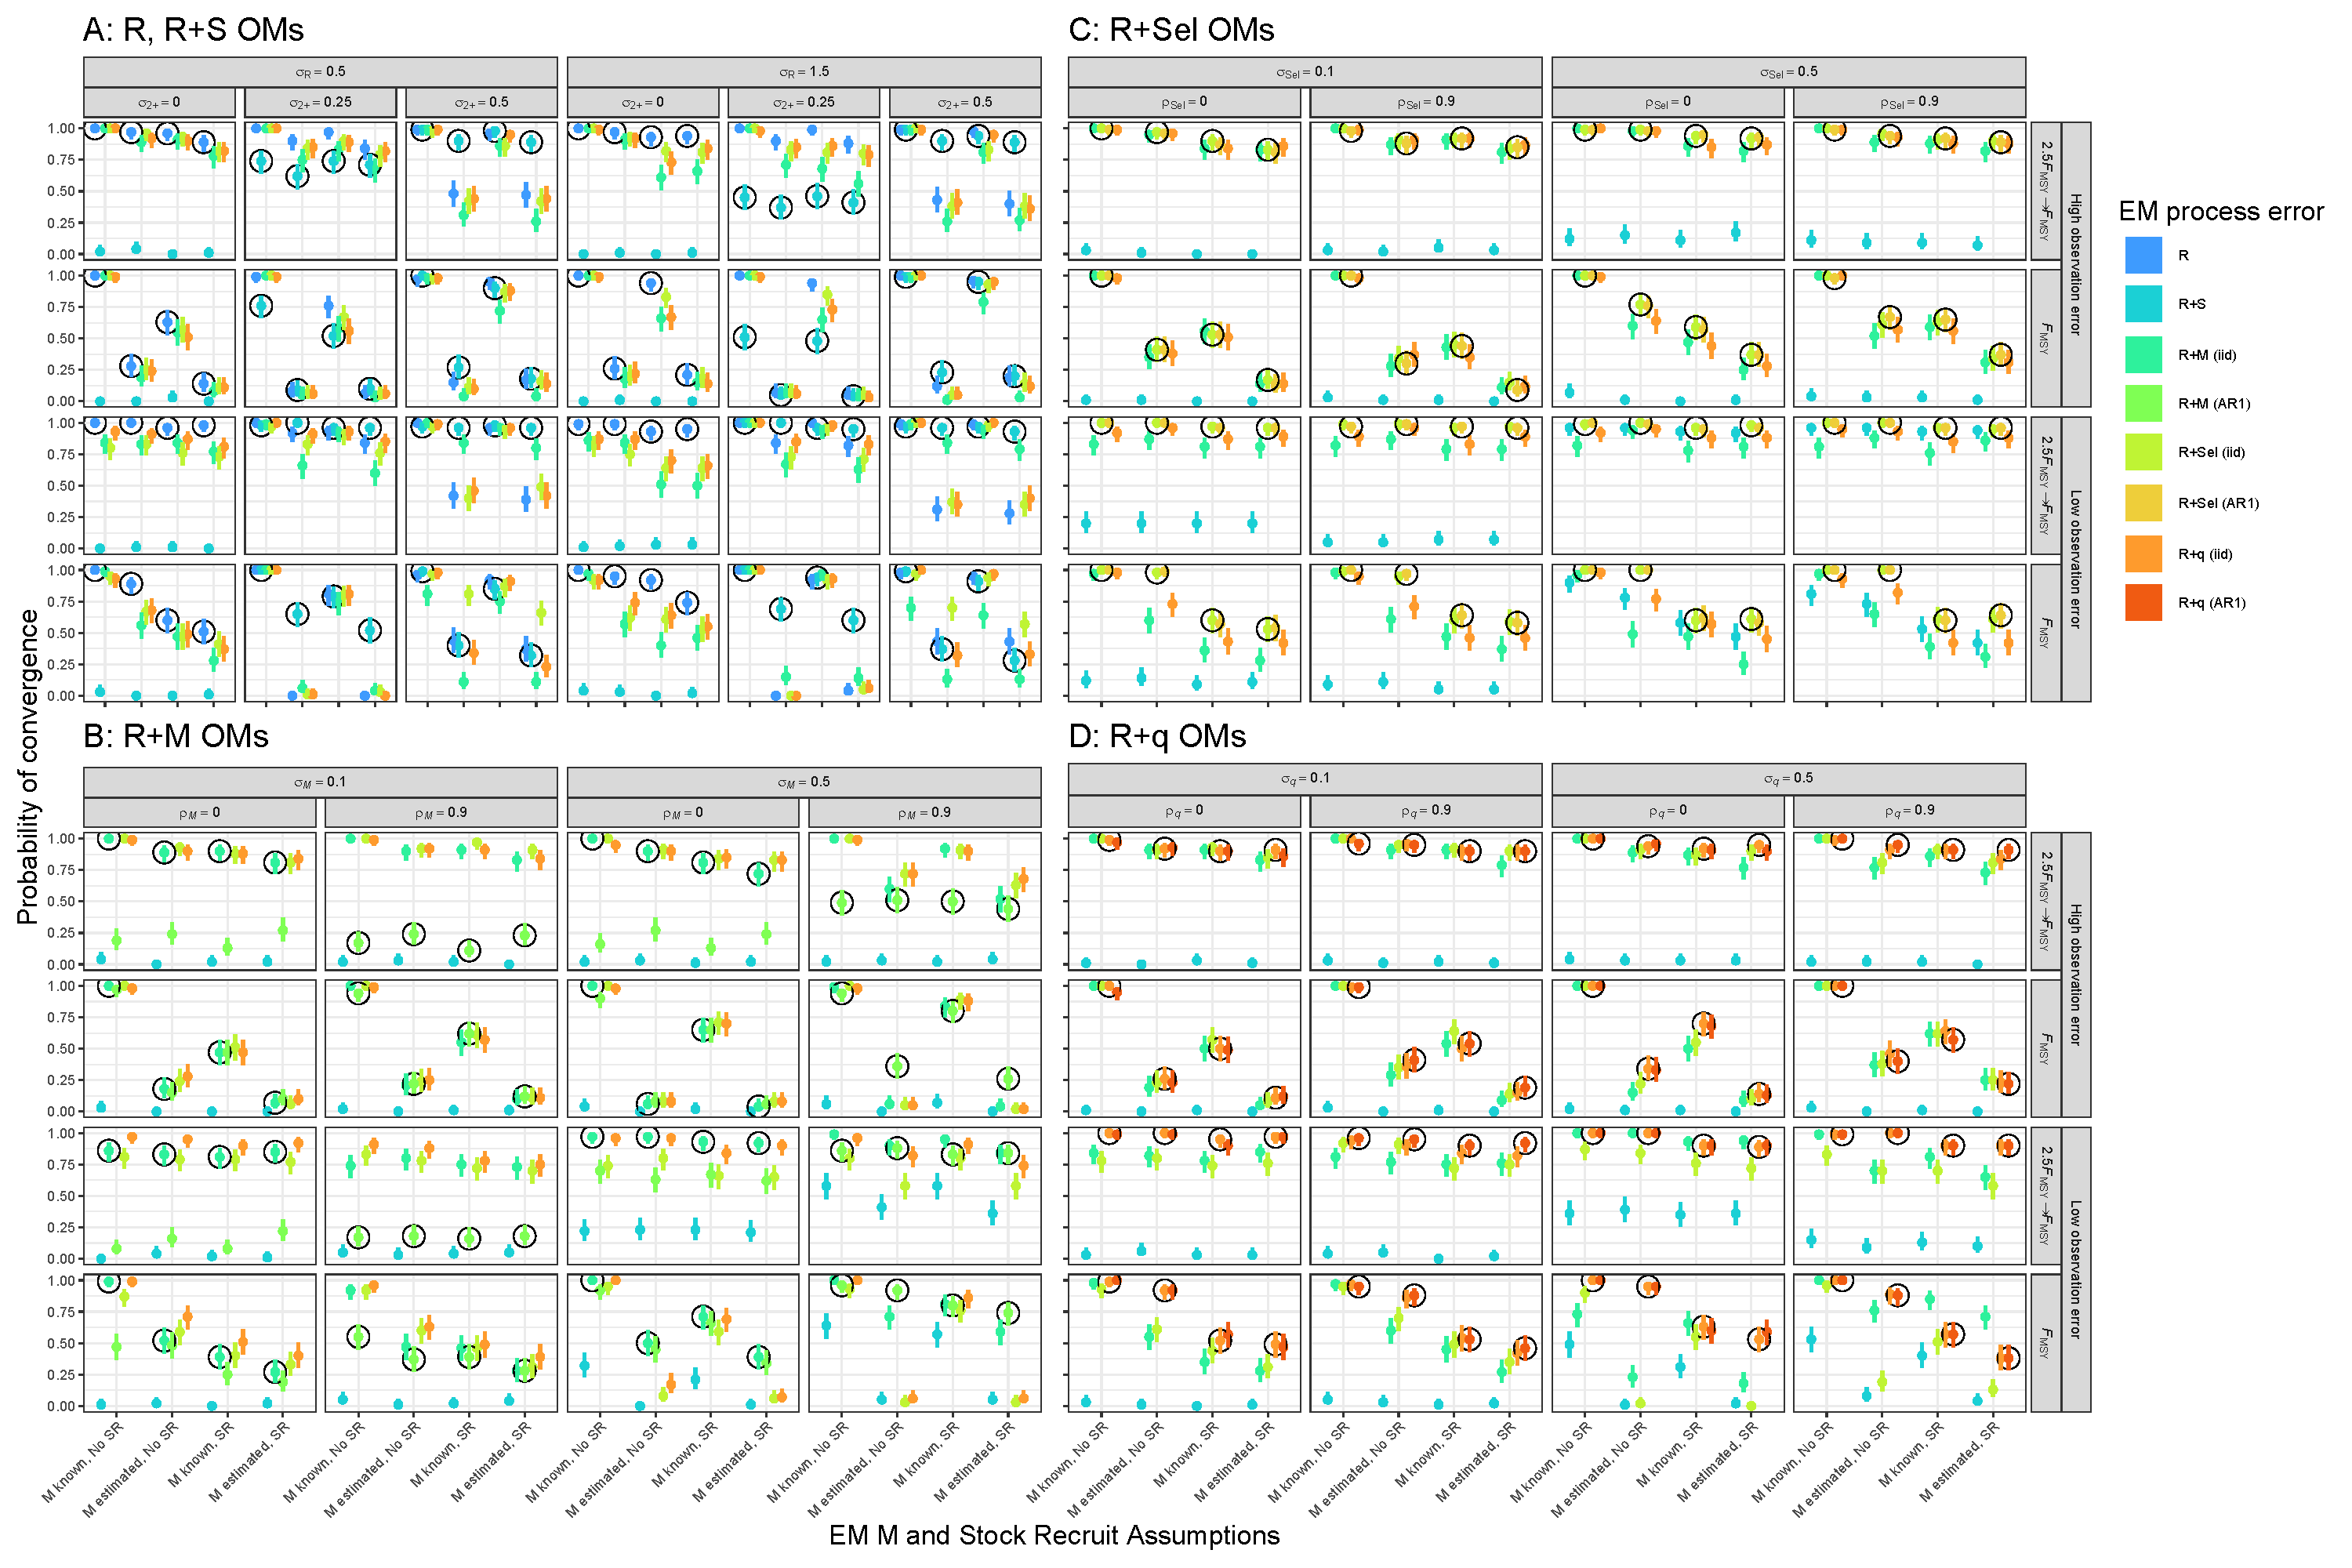
\includegraphics{type_3_convergence_plots}
\end{center}
\caption{Probability of estimating models providing maximum absolute values of gradients less than $10^{-6}$ assuming alternative process error (colored points and lines), and median natural mortality (estimated or known) and Beverton-Holt stock recruit functions (estimated or not; along x-axis) when fitted to operating models that have R and R+S (A), R+Sel (B), R+M (C), or R+q (D) process error structures. Circled values indicate results where the EM process error structure matches that of the operating model and vertical lines represent 95\% confidence intervals.}\label{gradient_convergence}
\end{figure}
\end{landscape}

\clearpage

\begin{landscape}
\begin{figure}
\begin{center}
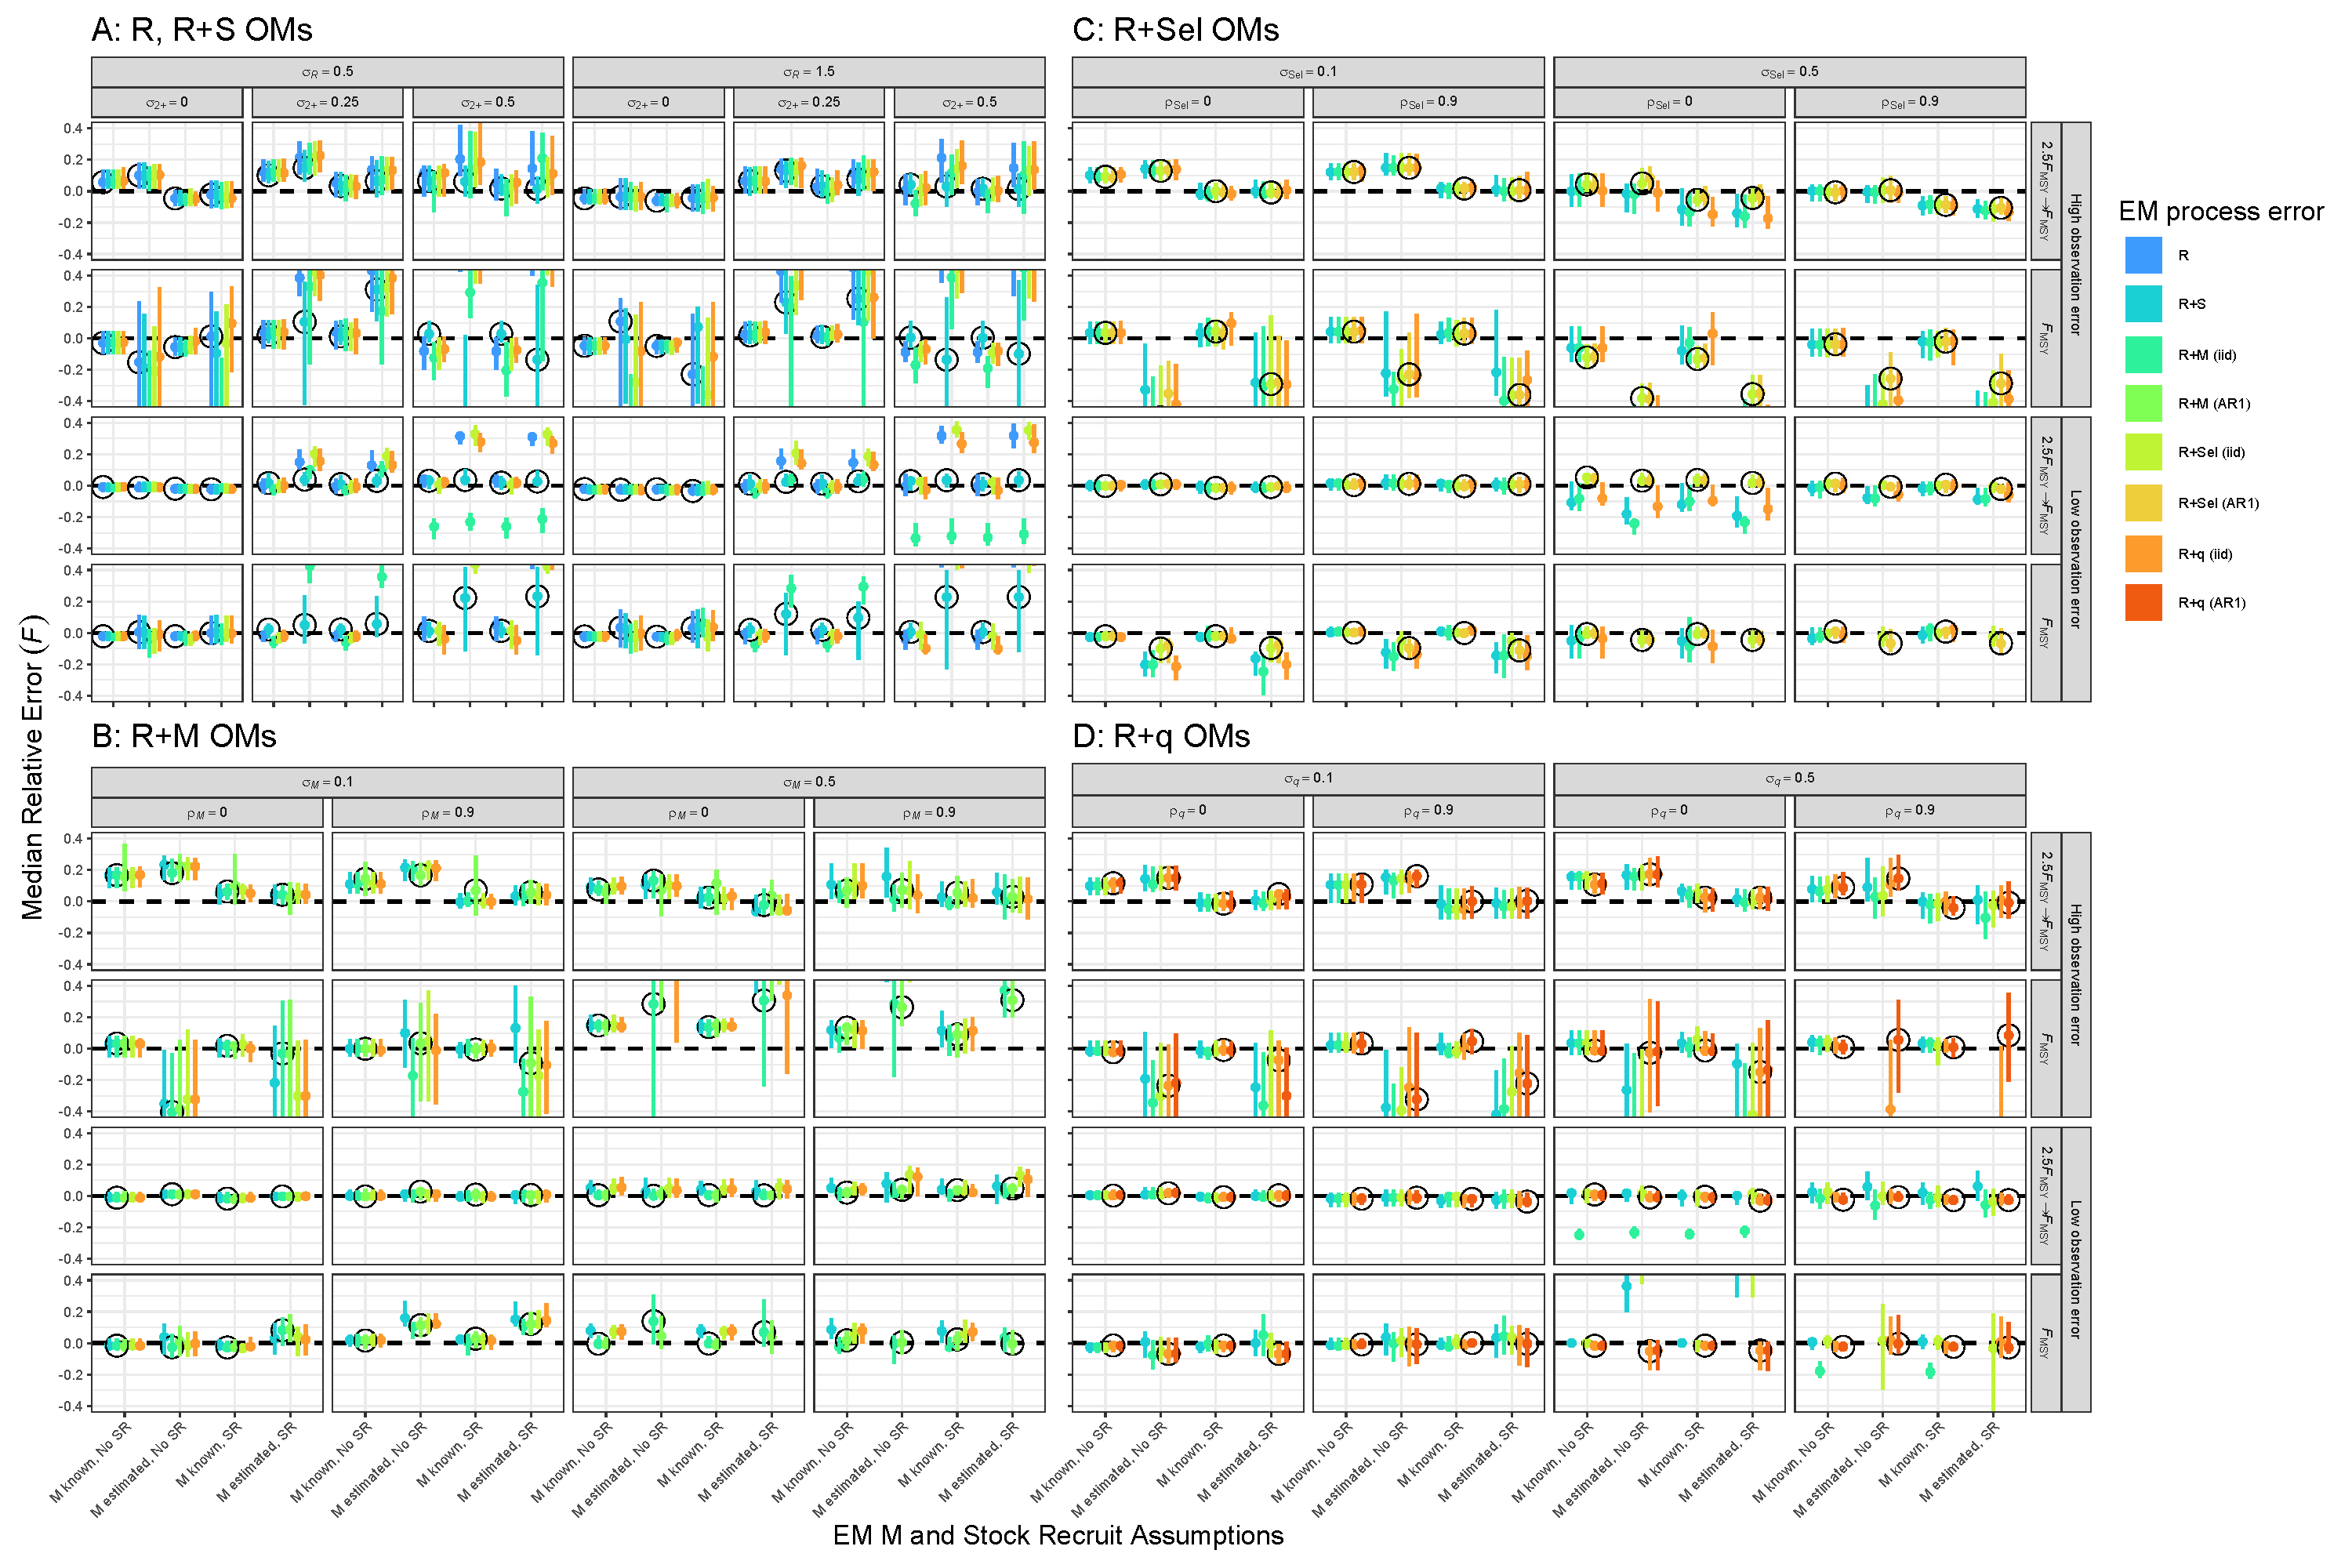
\includegraphics{term_F_bias_plots}
\end{center}
\caption{Median relative error of terminal year fully-selected fishing mortality for estimating models fitted to data sets simulated with alternative process error structures: R and R+S (A), R+Sel (B), R+M (C), or R+q (D). Circled values indicate results where the EM process error structure matches that of the operating model and vertical lines represent 95\% confidence intervals.}\label{F_rel_error}
\end{figure}
\end{landscape}

\begin{landscape}
\begin{figure}
\begin{center}
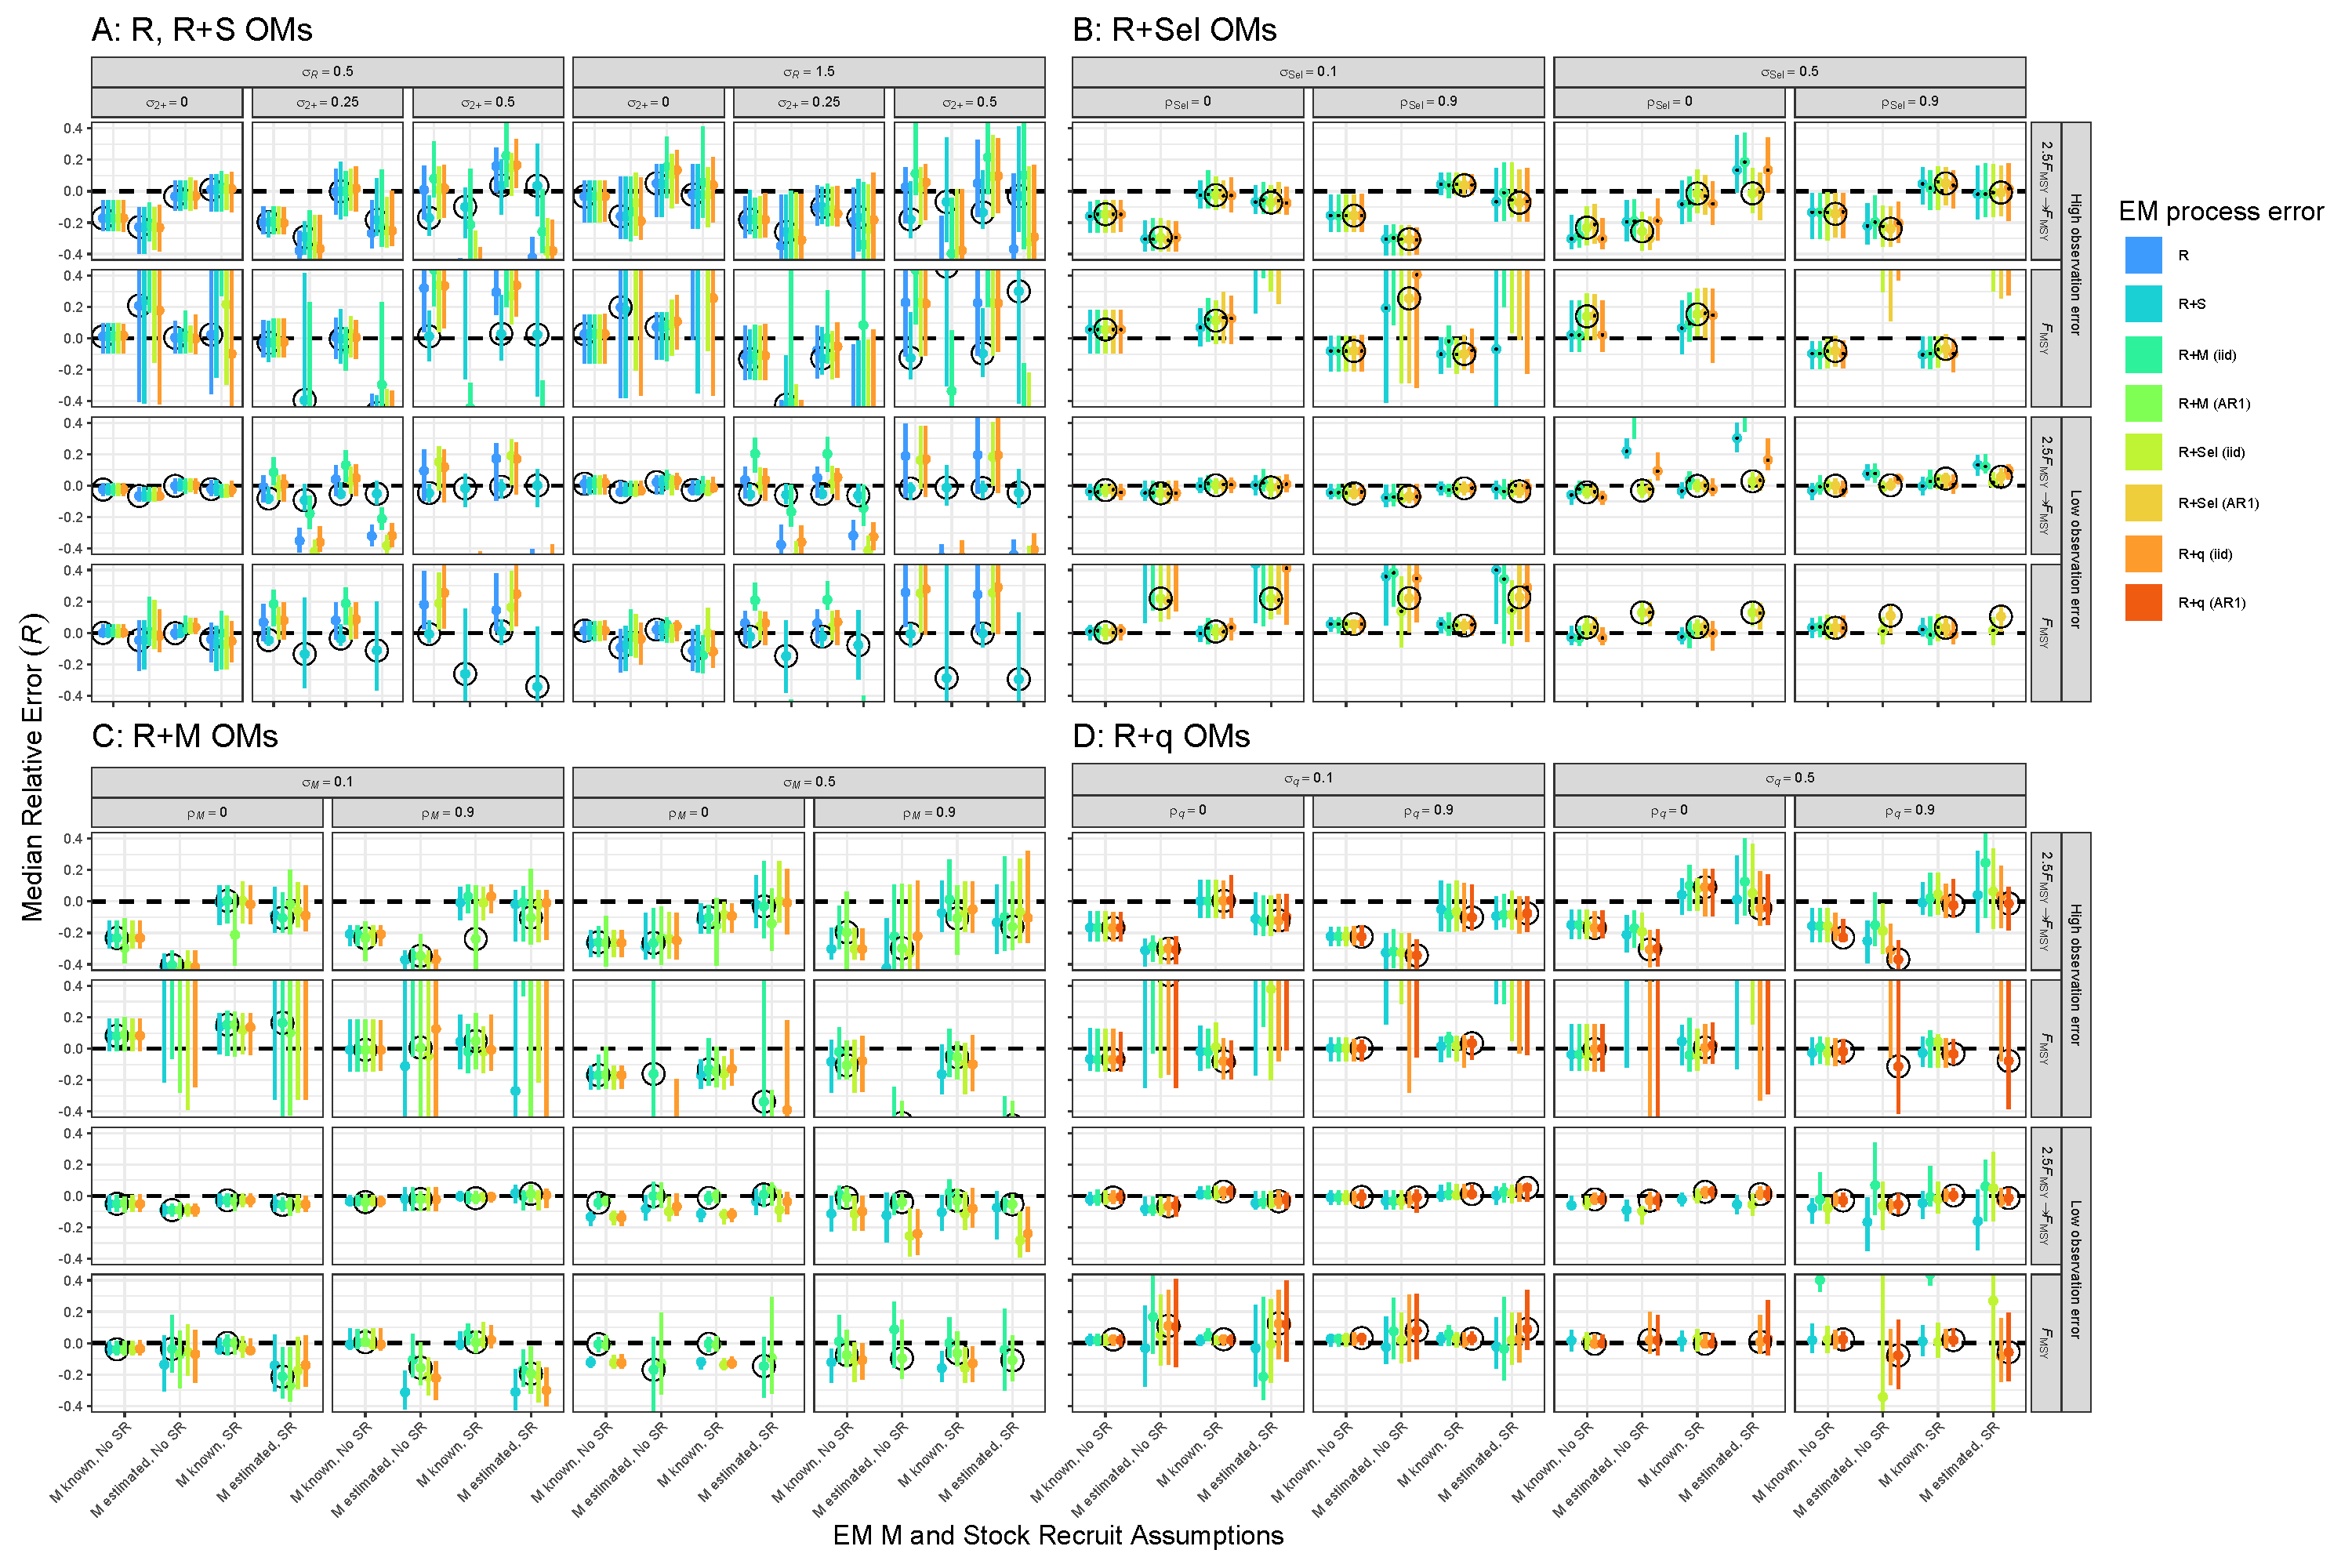
\includegraphics{term_R_bias_plots}
\end{center}
\caption{Median relative error of terminal year recruitment for estimating models fitted to data sets simulated with alternative process error structures: R and R+S (A), R+Sel (B), R+M (C), or R+q (D). Circled values indicate results where the EM process error structure matches that of the operating model and vertical lines represent 95\% confidence intervals.}\label{R_rel_error}
\end{figure}
\end{landscape}

\begin{landscape}
\begin{figure}
\begin{center}
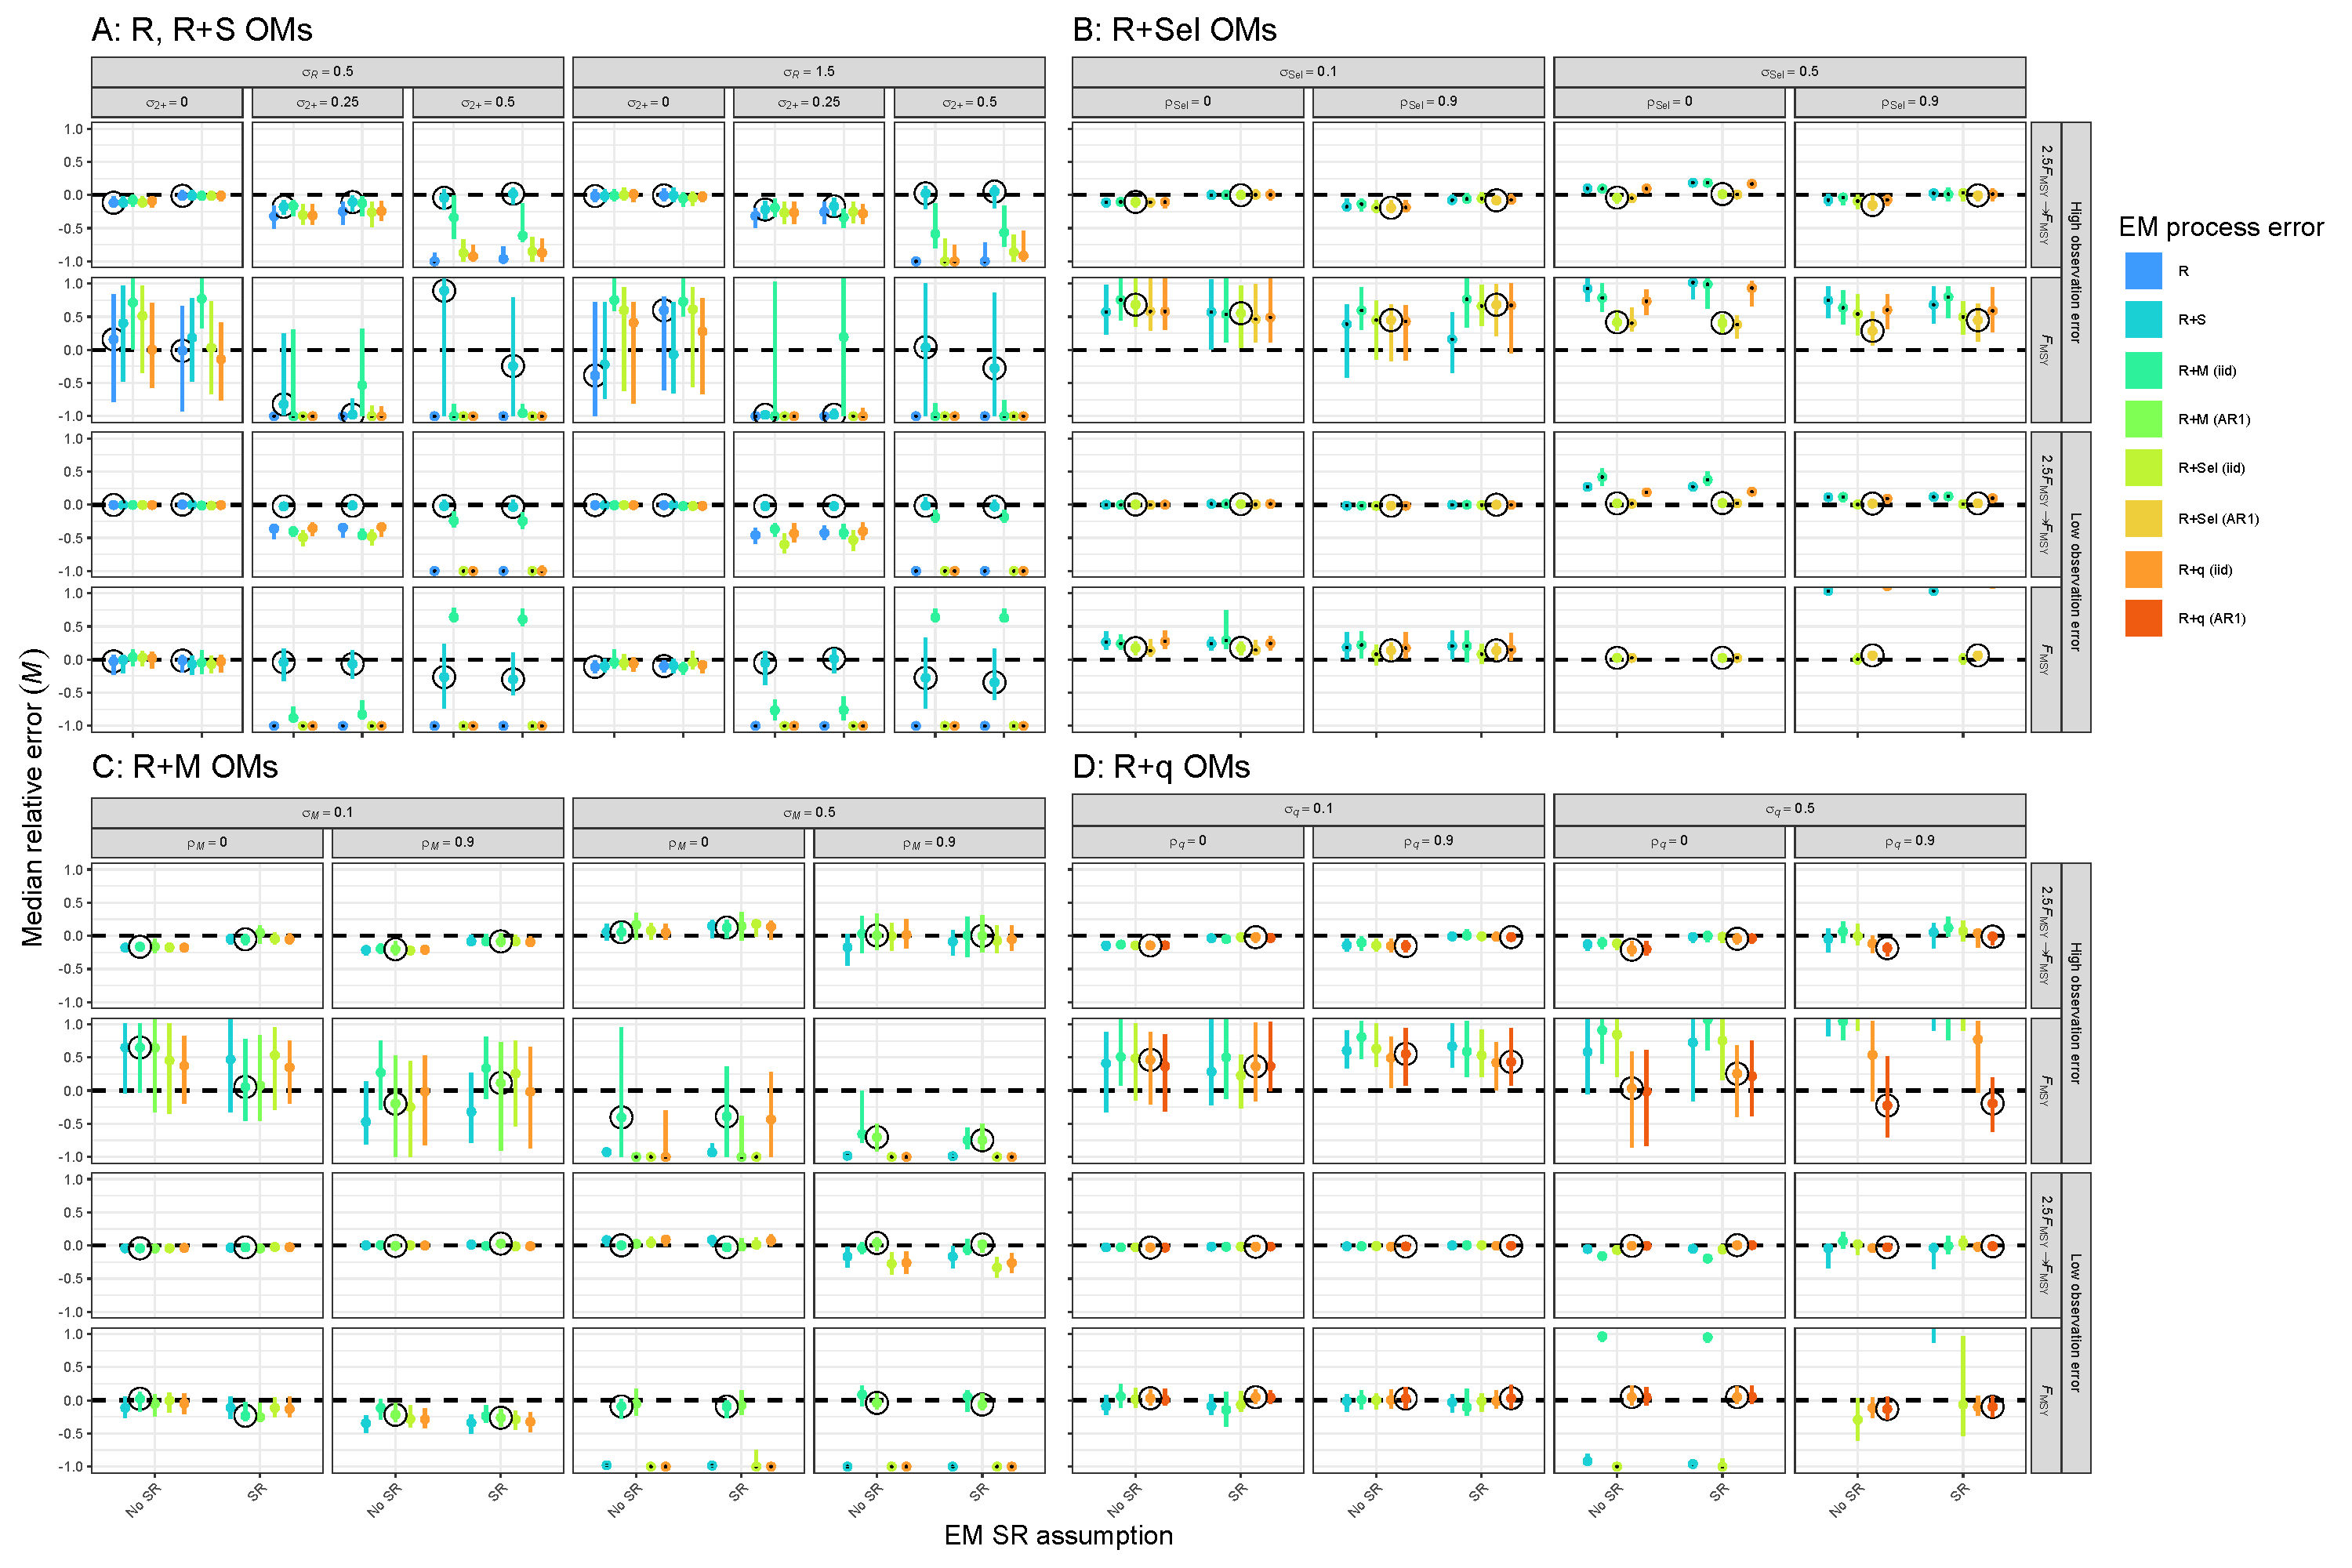
\includegraphics{M_bias_plots}
\end{center}
\caption{Median relative error of median/constant natural mortality for estimating models fitted to data sets simulated with alternative process error structures: R and R+S (A), R+Sel (B), R+M (C), or R+q (D). Circled values indicate results where the EM process error structure matches that of the operating model and vertical lines represent 95\% confidence intervals.}\label{M_rel_error}
\end{figure}
\end{landscape}

\begin{landscape}
\begin{figure}
\begin{center}
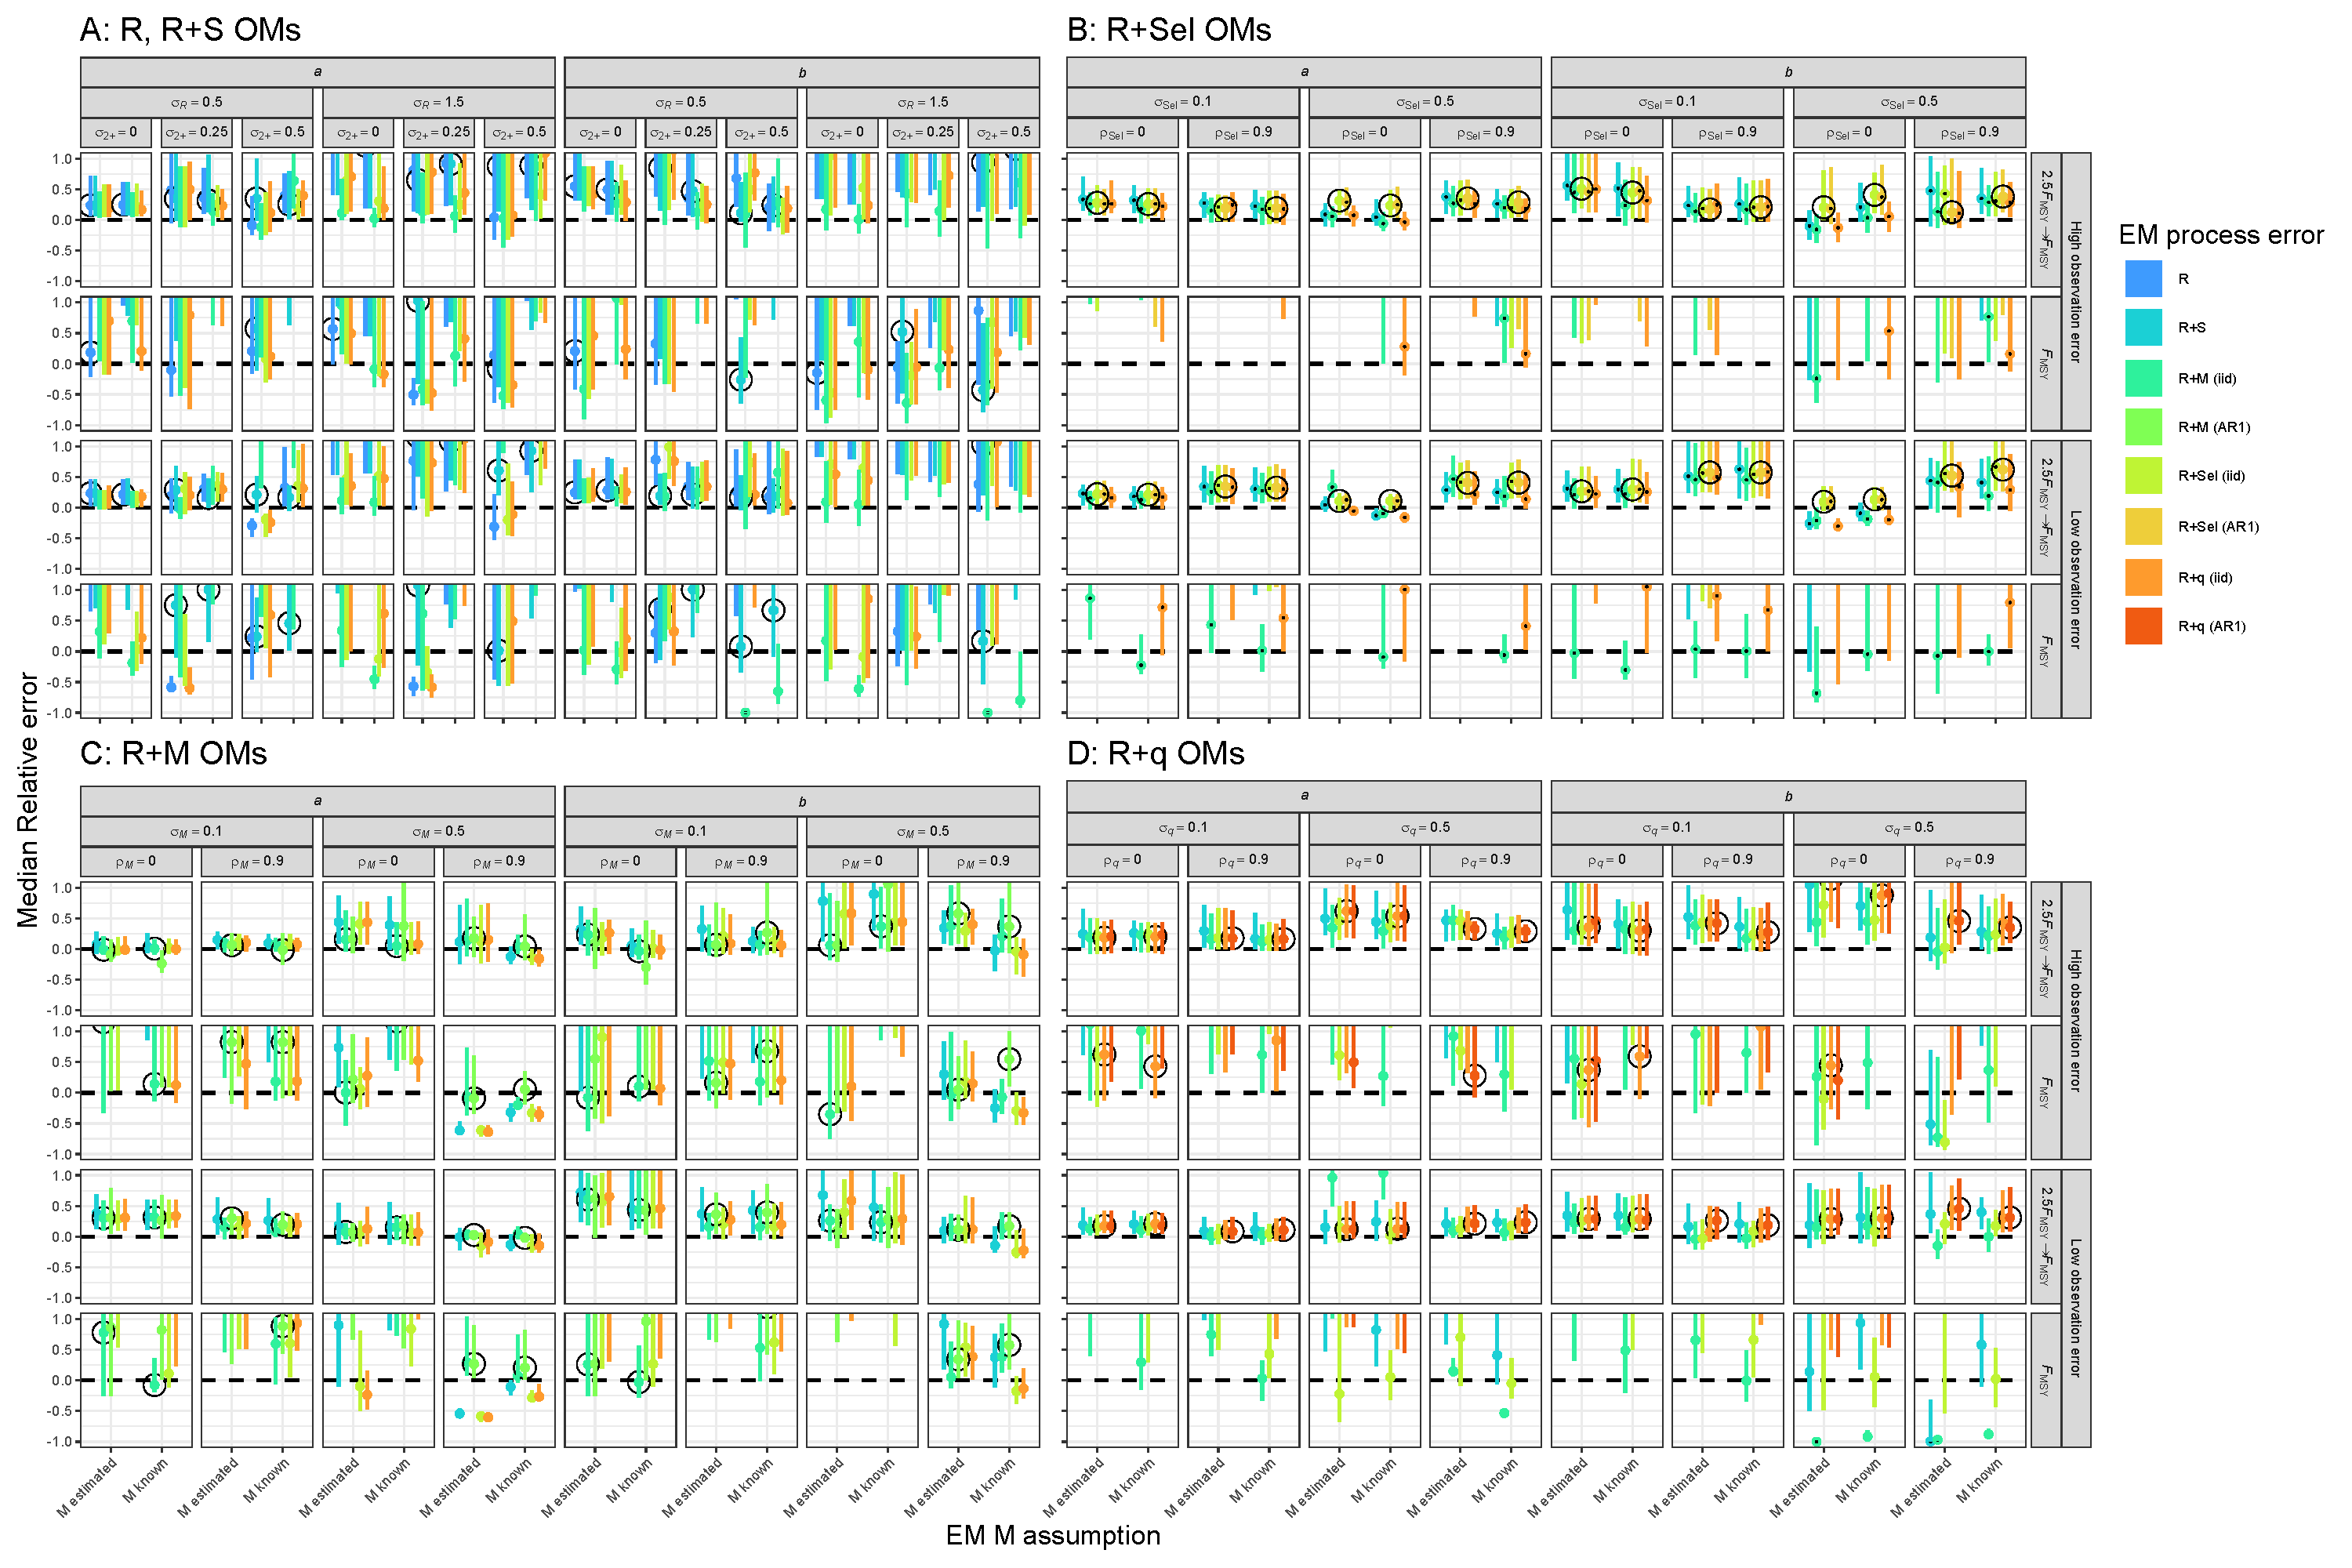
\includegraphics{sr_bias_plots}
\end{center}
\caption{Median relative error of Beverton-Holt stock recruitment parameters ($a$ and $b$) for estimating models fitted to data sets simulated with alternative process error structures: R and R+S (A), R+Sel (B), R+M (C), or R+q (D). Circled values indicate results where the EM process error structure matches that of the operating model and vertical lines represent 95\% confidence intervals.}\label{SR_rel_error}
\end{figure}
\end{landscape}

\begin{landscape}
\begin{figure}
\begin{center}
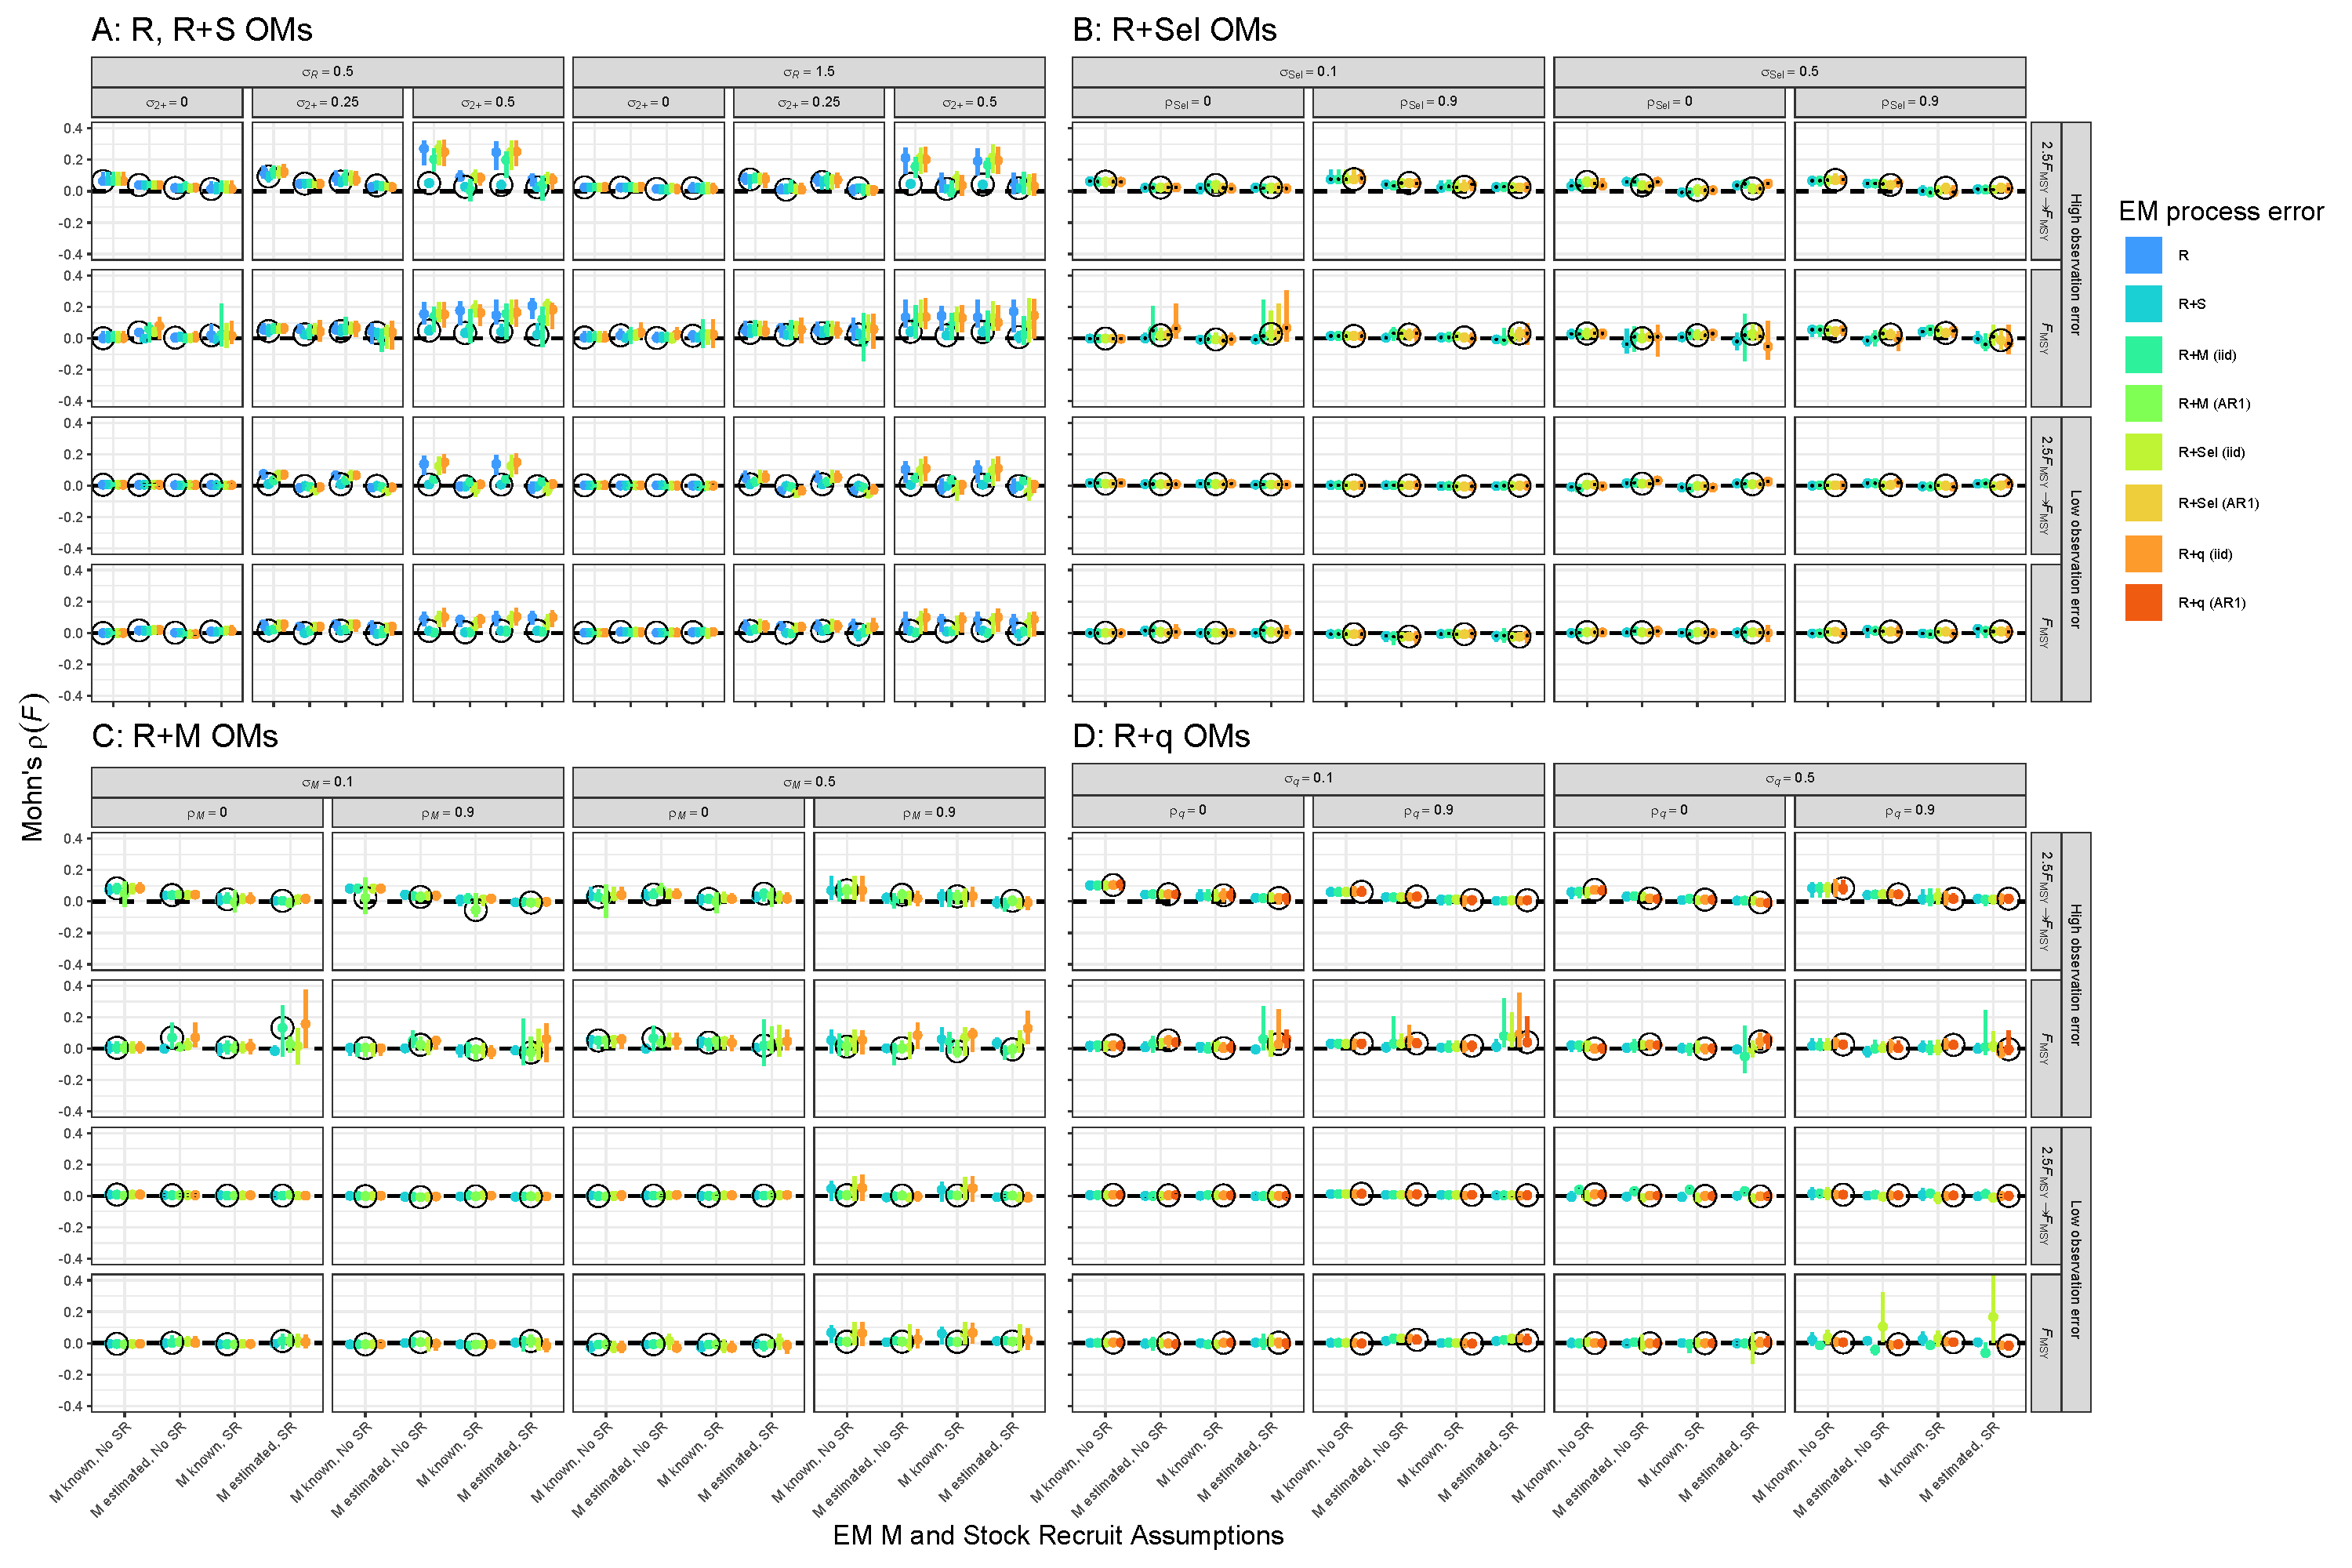
\includegraphics{mohns_rho_F_plots}
\end{center}
\caption{Median Mohn's $\rho$ of fishing mortality averaged over all age classes for estimating models fitted to data sets simulated with alternative process error structures: R and R+S (A), R+Sel (B), R+M (C), or R+q (D). Circled values indicate results where the EM process error structure matches that of the operating model and vertical lines represent 95\% confidence intervals.}\label{mohns_rho_F}
\end{figure}
\end{landscape}

\begin{landscape}
\begin{figure}
\begin{center}
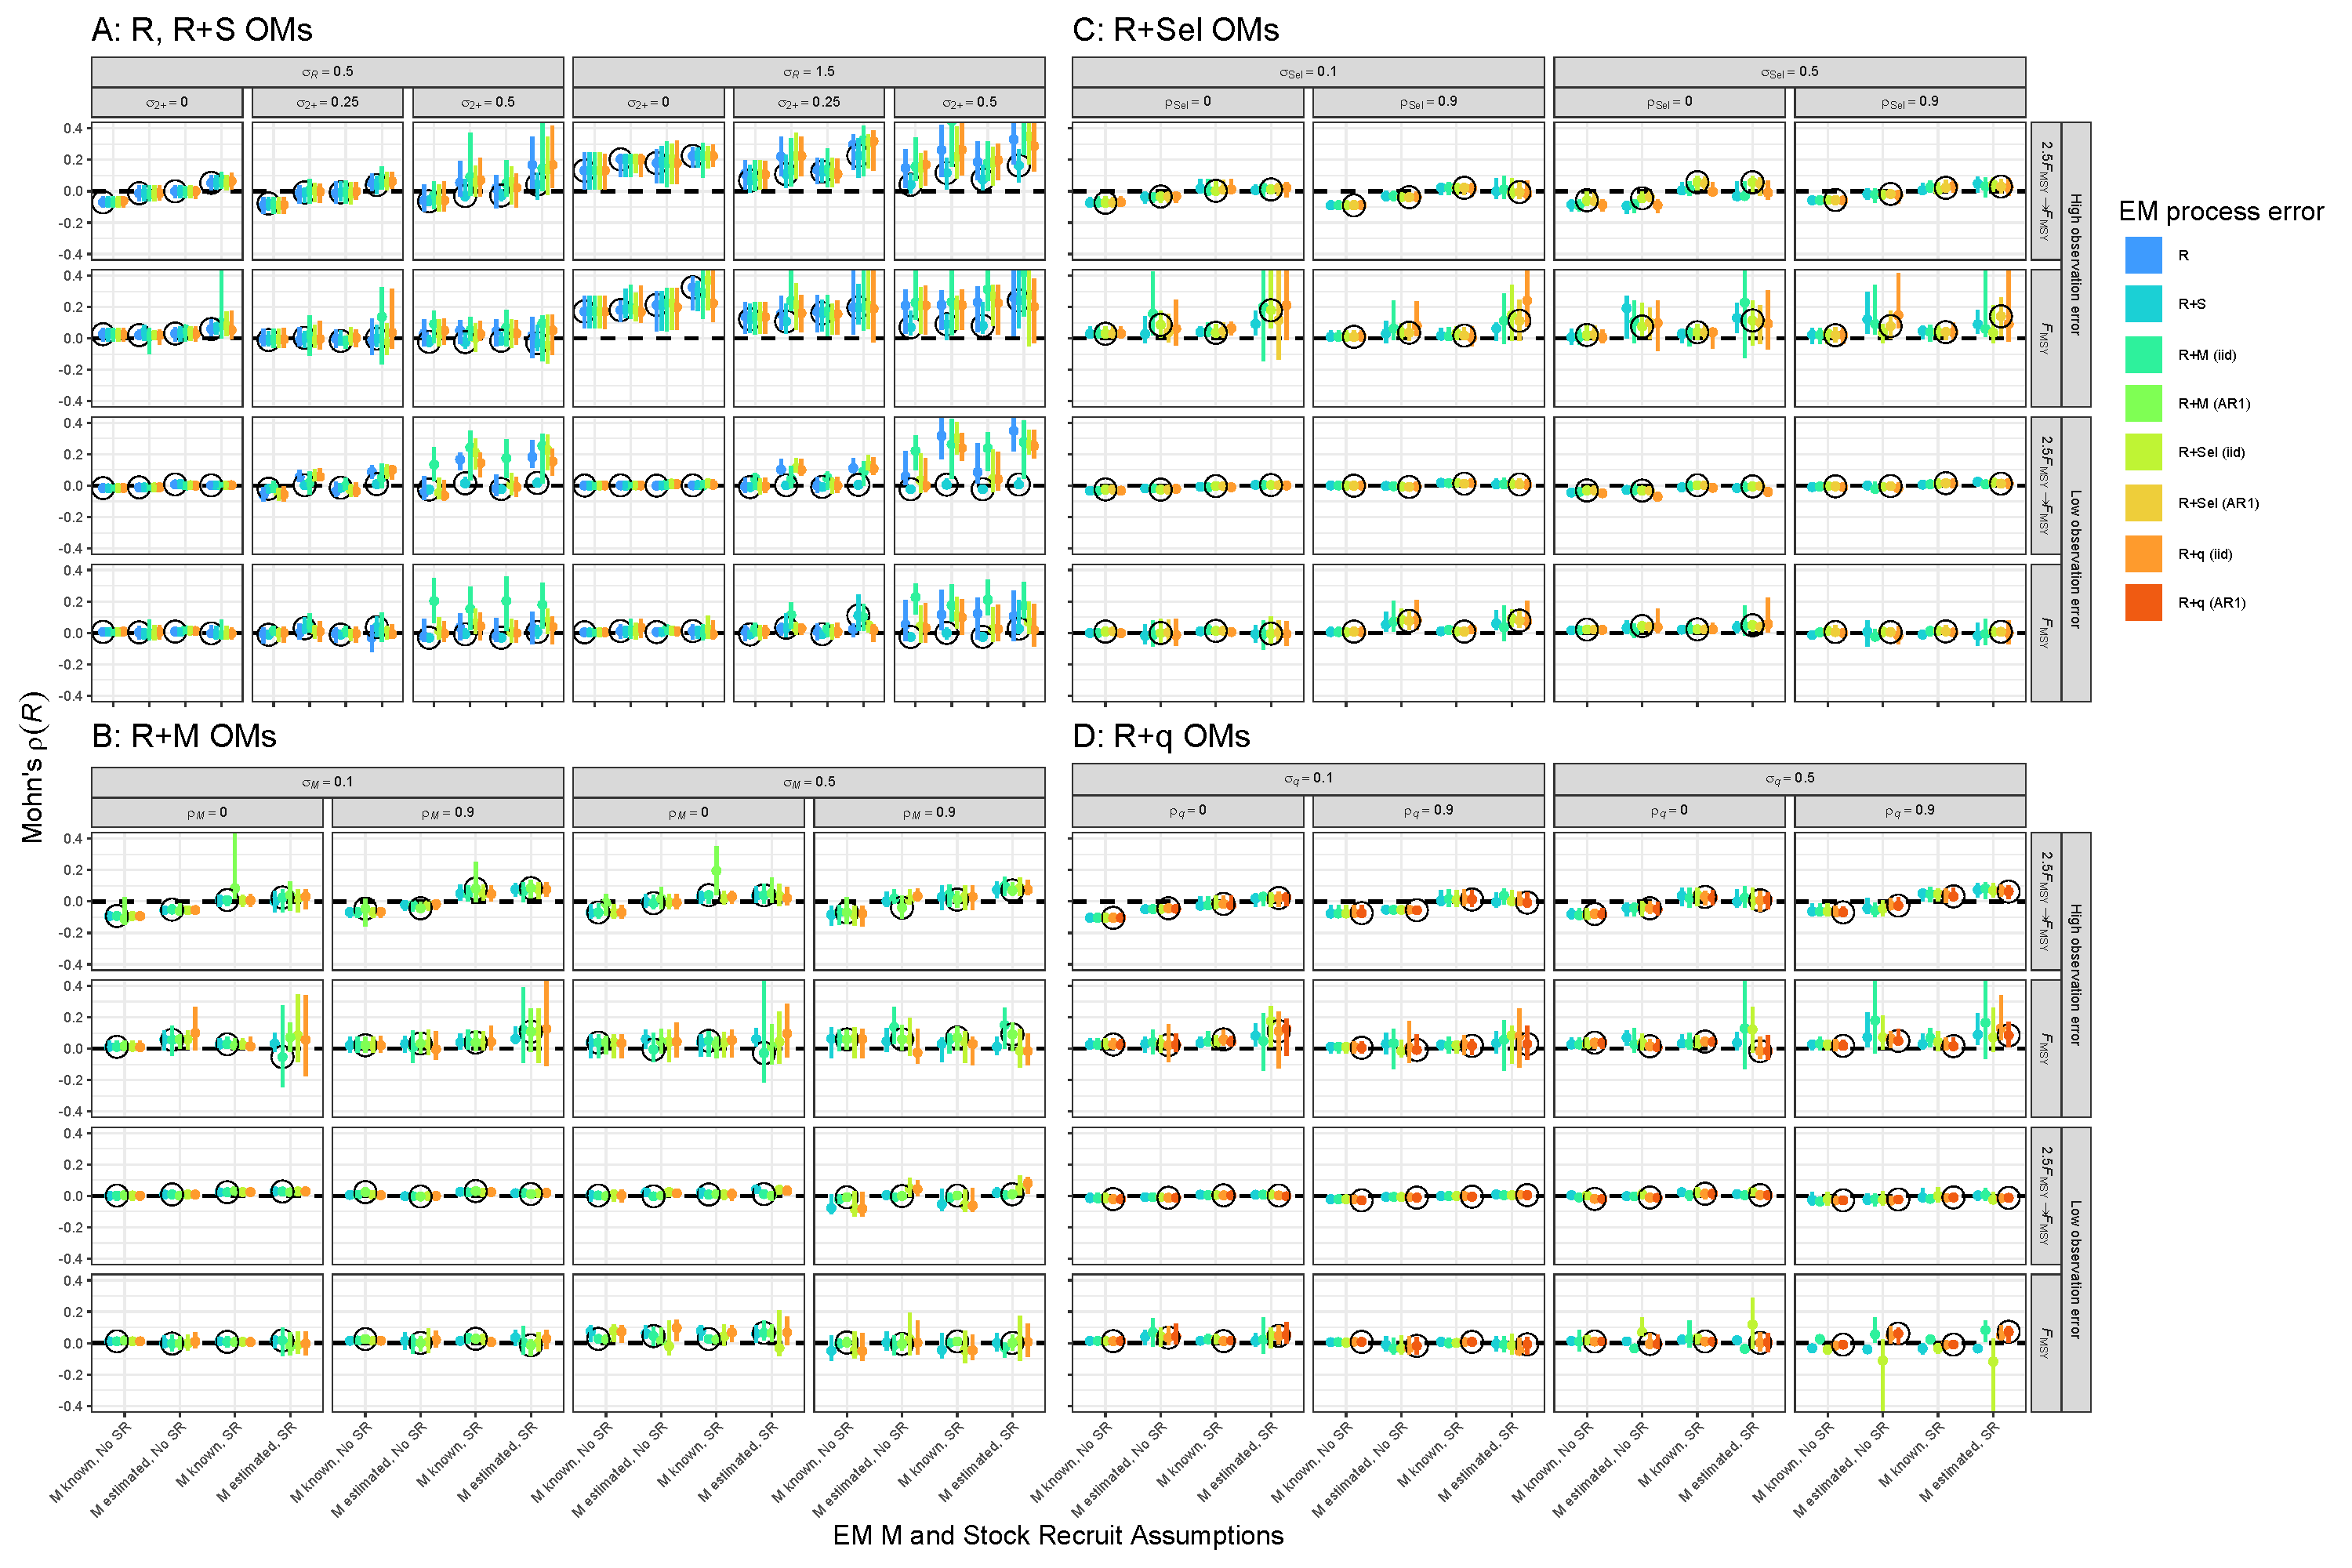
\includegraphics{mohns_rho_R_plots}
\end{center}
\caption{Median Mohn's $\rho$ of recruitment for estimating models fitted to data sets simulated with alternative process error structures: R and R+S (A), R+Sel (B), R+M (C), or R+q (D). Circled values indicate results where the EM process error structure matches that of the operating model and vertical lines represent 95\% confidence intervals.}\label{mohns_rho_F}
\end{figure}
\end{landscape}

\end{document}
